\documentclass[11pt,a4paper]{report}
\usepackage{afterpage}
\usepackage{hyperref}
\hypersetup{
colorlinks,
allcolors=black,
linktoc=all
}
\usepackage{titlesec}
\titleformat{\chapter}[display]{\vspace{-3cm}\normalfont\bfseries}{}{0pt}{\LARGE}
\usepackage[english,main=spanish]{babel}
\usepackage[utf8]{inputenc}
\usepackage{color}
\usepackage[table]{xcolor}
\usepackage{graphicx}
\usepackage[export]{adjustbox}
\usepackage{amssymb}
\usepackage{url}
\usepackage{xcolor}
\usepackage{caption}
\usepackage{float}
\usepackage{listingsutf8}
\usepackage[framemethod=default]{mdframed}
\definecolor{LightGray}{gray}{0.9}
\usepackage{babel}
\usepackage[english]{babelbib}

\usepackage{caption}
\usepackage{subcaption}

\definecolor{codegreen}{rgb}{0,0.6,0}
\definecolor{codegray}{rgb}{0.5,0.5,0.5}
\definecolor{codepurple}{rgb}{0.58,0,0.82}
\definecolor{backcolour}{rgb}{0.95,0.95,0.92}
\lstdefinestyle{codigo}{
    backgroundcolor= \color{backcolour},   
    commentstyle=\color{codegreen},
    keywordstyle=\color{magenta},
    numberstyle=\tiny\color{codegray},
    stringstyle=\color{codepurple},
    basicstyle=\scriptsize\normalfont\sffamily,  
    breakatwhitespace=false,         
    breaklines=true,                 
    captionpos=t,                 
    keepspaces=true,
    numbers=left,                   
    numbersep=5pt,  
    showspaces=false,                
    showstringspaces=false,
    showtabs=false,                  
    tabsize=2,
    frame=single,
    framexleftmargin=5pt,
    framexrightmargin=3pt,
    framexbottommargin=3pt,
    framextopmargin=3pt,
    inputencoding=utf8,
    extendedchars=true,
    literate = {¬}{{$\neg$}}1
}

\DeclareCaptionFormat{listing}{#1#2#3}
\captionsetup[lstlisting]{format=listing,singlelinecheck=false, margin=0pt, font={sf},labelsep=space,labelfont=bf}


\renewcommand{\lstlistingname}{Código}
\renewcommand{\lstlistlistingname}{Índice de códigos}

\usepackage[many]{tcolorbox}  
\newtcolorbox{boxB}{
    boxrule = 1.5pt,
    colframe = white,
    rounded corners,
    arc = 5pt
}

\definecolor{mygreen}{rgb}{0,0.6,0}
\definecolor{mygray}{rgb}{0.5,0.5,0.5}
\definecolor{mymauve}{rgb}{0.58,0,0.82}
\definecolor{terminalbgcolor}{HTML}{330033}
\definecolor{terminalrulecolor}{HTML}{000099}

\lstdefinestyle{terminal}
{
    backgroundcolor=\color{black},
	basicstyle=\scriptsize\color{white}\ttfamily,
	breaklines=true,
	captionpos=t,
	extendedchars=true,
	showspaces=false,
	showstringspaces=false,
	frame=single,
    framexleftmargin=5pt,
    framexrightmargin=5pt,
    framexbottommargin=5pt,
    framextopmargin=5pt,
    breakindent=0pt,
    breakautoindent=false,
    literate={\$}{{\$}}1 
         {:}{{:}}1
         {¬}{{$\neg$}}1
         {~}{{\textasciitilde}}1,
}

\begin{document}

% \begin{titlepage}
\begin{center}


\includegraphics[height=2.38cm]{imagenes/logo_uc.png}
\vspace{0.4cm}

\textbf{Facultad de Ciencias}

\vspace{1cm}

\LARGE
\textbf{Modelado del caudal natural en la cuenca hidrográfica Chambo con Redes Neuronales}

Título en inglés

\vspace{1.cm}
Trabajo de Fin de Máster


\vspace{0.5cm}
\textbf{Anabela Romina Turlione}

\vspace{0.3cm}
\small
\textbf{Director }: Felipe Fernandez Perez\\
\textbf{co Director }: Manuel de Jesus Peñil




% \Large
% Facultad de Informática\\
% Universidad Nacional de La PLata
\end{center}


% \begin{figure}[t]
%     \raggedright
%       
\includegraphics[scale=1]{Figures/Portada.pdf}
        
%   \end{figure}


\end{titlepage}
%  \afterpage{\null\thispagestyle{empty}\newpage}
 %\chapter*{Agradecimientos}
\markboth{AGRADECIMIENTOS}{AGRADECIMIENTOS}
\thispagestyle{empty}
Página de agradecimientos

\tableofcontents
\thispagestyle{empty}

% \lstlistoflistings
% \thispagestyle{empty}

\listoffigures
\thispagestyle{empty}

\setcounter{page}{1}
\chapter*{Resumen}
\addcontentsline{toc}{chapter}{Resumen}

En este trabajo se ha evaluado el desempeño de diferentes modelos de redes neuronales
para predecir el caudal natural en la cuenca hidrográfica Chambo  a partir de series de
entrada hidro-climáticas que abarcan un rango de 14 años. Se han considerados redes con
diferentes estructuras y se han entrenado de manera local, global y secuencial. Se ha medido el
desempeño de los modelos utilizando diferentes métricas y se ha comprobado que en la
mayoría de los casos, los modelos logran reconstruir de manera correcta los caudales en un
rango de 6 años. Con los resultados obtenidos se ha utilizado el software de gestión Modsim
que permite optimizar los usos de los recursos de la cuenca y se ha comprobado que los
resultados obtenidos por medio de los modelos de redes neuronales son los mismos que los obtenidos con un
modelo hidrológico tradicional. Finalmente se ha desarrollado una aplicación que permite la ejecución del modelo
en diferente cuencas hidrológicas.\\
\\
\textbf{Palabras claves:} Redes Neuronales, redes recurrentes, hidrología, predicción, cuencas hidrográficas, aprendizaje automático, aprendizaje profundo\\
\\
\\
\large{\textbf{Abstract}}
\vspace{5mm}

In this work, the performance of different neural network models
to predict the natural flow in the  watershed Chambo  has been evaluated. 
Models with different configurations  have been trained locally, globally and sequentially  in 
hydro-climatic series spanning a 14-year range.
The performance of the models, has been measured
using different metrics, and it has been verified that in most cases, they succeed in correctly reconstructing the flows over a
6 year range. The obtained results  has been used to optimize the use of the resources of the basin with the software Modsim, 
and it has been proven that the the results obtained by means of neural network models are the same as those obtained with a
traditional hydrological model. Finally, an application has been developed that allows the execution of the model
in different hydrological basins.\\
\\
\textbf{Key words:} Neural Networks, recurrent networks, hydrology, prediction, hydrographic basin, machine learning, deep learning
\chapter{Introducción}
\label{introduccion}

Introducción de la tesis

Ejemplo de secciones

\section{Motivación}

Motivación de la tesis.

Un ejemplo de cita.\cite{web:unlp}

\section{Objetivos y metodología}

Objetivos y metodología.

\section{Resultados obtenidos}

Resultados obtenidos

\section{Organización del documento}

Organización del documento

\begin{itemize}
    \item Capítulo 1.
    \item Capítulo 2.
    \item Capítulo 3.
\end{itemize}
% \chapter{Cuenca del río Chambo}
\label{capitulo 1}
\section{Descripción del sistema}
% \section{Red fluvial}
% \section{Usos de agua}
% \section{Aportaciones}
\chapter{Descripción y exploración de los datos}
\label{capitulo 1}


En este capítulo se describen las características principales de las series temporales hidroclimáticas utilizadas 
tanto para entrenar los modelos de aprendizaje profundo como para generar las variables objetivos, es describe
los caudales de descarga de las subcuencas con el modelo hidrológico LEM.



\section{Series de precipitación}


La cuenca del río Chambo posee una gran variación en la precipitación en un área geográfica reducida,
por este motivo los valores de precipitación recogidos por pluviómetros en las estaciones meteorológicas 
pueden no son fácilmente extrapolables a puntos más lejanos. Por otro lado los pluviómetros se encuentran 
a altitudes de entre los 2000 y 3000 metros sobre el nivel del mar, mientras que el punto más alto de la cuenca se encuentra a las 6288 m.s.n.m,
Lo que da lugar a que haya una deficiencia de datos en ciertos puntos geográficos de la cuenca. Para completar los datos en Estos
puntos se ha recurrido a las base de datos de ERA5 \cite{ERA5} y CHELSA \cite{CHELSA}.


Con el fin de contrastar si estas series reflejan 
correctamente las variaciones del patrón de lluvias con la altura y la pendiente, 
se han analizado diversas bases de datos globales de precipitación pero el resultado no ha sido 
satisfactorio.  Por ello, se ha optado por generar las series de precipitación de manera sintéticas basándose 
en los patrones combinados de los pluviómetros y de las estaciones de aforos.



% Los datos de clima (precipitación y temperatura) fueron medidos a través de estaciones meteorológicas distribuidas de manera 
% irregular a lo largo de la cuenca. Las series disponibles reflejan adecuadamente las condiciones climáticas de las zonas 
% bajas y más pobladas, pero la información en las zonas más altas es escasa. 
% Los pluviómetros se encuentran a altitudes de entre los 2000 y 3000 metros sobre el nivel del mar, 
% mientras que el punto más alto de la cuenca se encuentra a las 6288 m.s.n.m

% Con el fin de contrastar si estas series reflejan 
% correctamente las variaciones del patrón de lluvias con la altura y la pendiente, 
% se han analizado diversas bases de datos globales de precipitación pero el resultado no ha sido 
% satisfactorio.  Por ello, se ha optado por generar las series de precipitación de manera sintéticas basándose 
% en los patrones combinados de los pluviómetros y de las estaciones de aforos.

% La cuenca del río Chambo posee una gran variación en la precipitación en un área geográfica reducida,
% por este motivo los valores de precipitación recogidos por pluviómetros en las estaciones meteorológicas 
% pueden no ser válidos para puntos lejanos. Es por eso que los datos correspondientes a puntos intermedios se 
% completaron a partir de la base de datos de ERA5 y CHELSA.

% \begin{figure}[h!]
%   \begin{center}
%     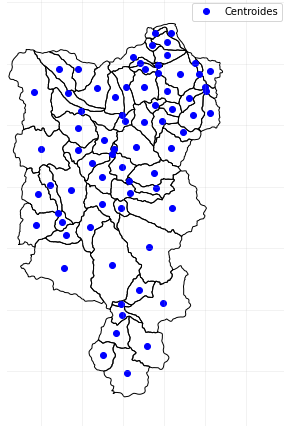
\includegraphics[height=3.in]{Figures/centroides.png}
%     \caption{ Localización de los centroides de las subcuencas}
%     \label{0}
%   \end{center}
% \end{figure}

%  Una vez que los huecos han sido rellenados, se han interpolado los datos recogidos por los pluviómetros a los centroides 
%  de las regiones  representadas en la figura \ref{0}. Este proceso consta de dos pasos, primero se estima si en un punto 
%  determinado va a llover (estimación kriging con la librería \textit{Krige} de r) y luego se estima la magnitud de dicha 
%  lluvia (Herrera et al., 2012).

%  \begin{figure}[h!]
%   \begin{center}
%     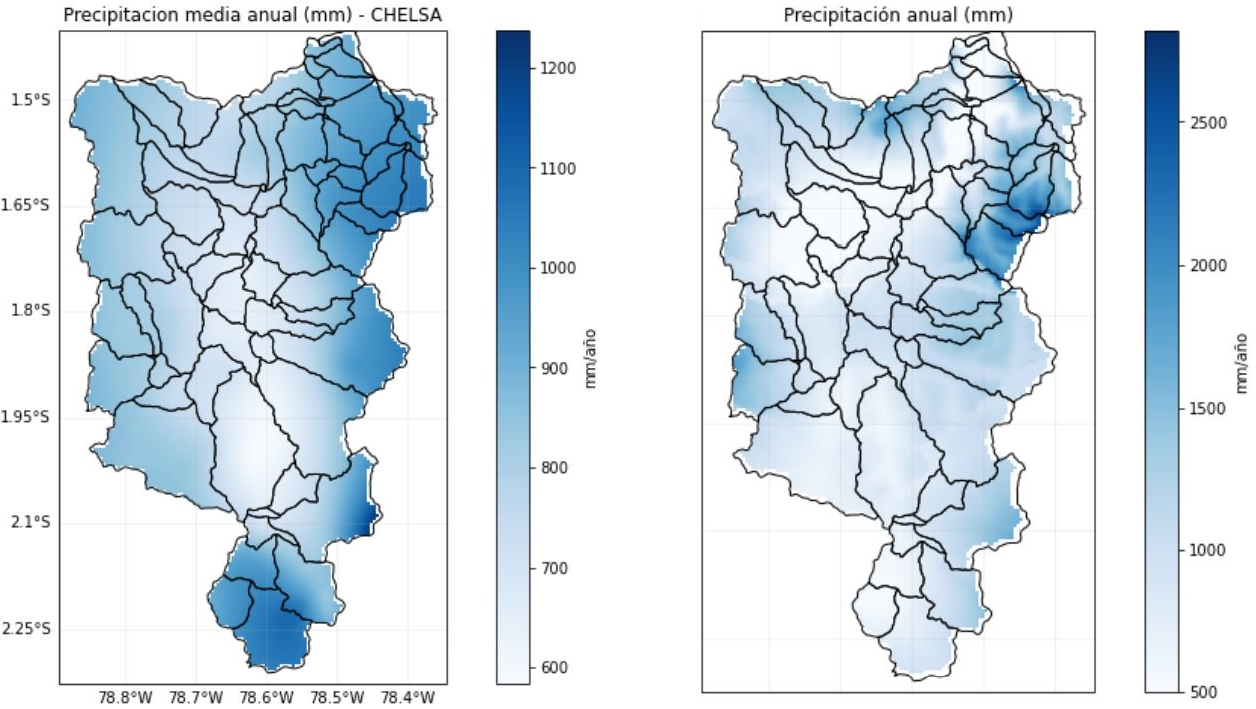
\includegraphics[height=3.in]{Figures/CHELSA_ERA5.jpg}
%     \caption{ Precipitación media anual (mm/año) basada en CHELSA (panel izquierdo) y en ERA5 (panel derecho).}
%     \label{1}
%   \end{center}
% \end{figure}


%  En la figura \ref{1} se muestra a modo de ejemplo los  valores de la precipitación media anual  obtenidos mediante interpolación 
%  sobre una malla regular de 100 m de lado utilizando la base de datos de ERA5 (panel derecho) y la de CHELSA (panel izquierdo).
%  Si bien los resultados reflejan correctamente la fuerte variabilidad de la precipitación en un area reducida, los patrones estacionales
%  así obtenidos no coinciden con los caudales y el conocimiento local. Es por eso que se ha optado por generar las series 
%  de manera sintética como se describe en la siguiente sección.



El modelo que genera las series de precipitación diaria consta de dos niveles, primero se generan series mensuales y
luego se generan series diarias desagregando los valores mensuales.
Para generar las series mensuales se parte del valor medio anual en la región de interés y del valor medio en el 
mes más húmero
% . Se han definido a su vez, tres patrones de precipitación para diferentes regiones:
% 1) costero, donde la precipitación máxima tiene lugar en el mes de abril, y un segundo pico inferior al de abril, en torno a octubre-noviembre.
% 2) amazónico, con un único pico de precipitación en junio-julio, y el mínimo en diciembre-enero y 3) mixto que es una combinación de los dos primeros. 

La precipitación media anual  se determina mediante en la interpolación de los datos de los
pluviómetros con la base de datos CHELSA ya que en términos de magnitud es la más exacta.
El modelo de desagregación a escala mensual asume que las precipitaciones acumuladas en cada mes siguen un comportamiento
que puede ser representado por la siguiente distribución "Log-normal" que posee una variación temporal sinusoidal y
desviación estándar $s_1$:

\begin{equation}
    P_m=exp\Bigg(N\bigg(a+b1\cdot cos\bigg(\frac{t-\phi_1}{6}\bigg)+b2\cdot cos\bigg(\frac{t-\phi_2}{12}\bigg)\bigg)\Bigg)
\end{equation}

$N(\mu,\sigma)$ es a su vez una distribución Gaussiana con media $\mu$ y desviación estándar $\sigma$. 
Los valores de las constantes $a$, $b_1$ y $b_2$ se obtienen a partir de la precipitación media y máxima, 
mientras que las fases $\phi_i$ dependen del régimen de precipitación.

% \begin{figure}[h!]
%     \begin{center}
%       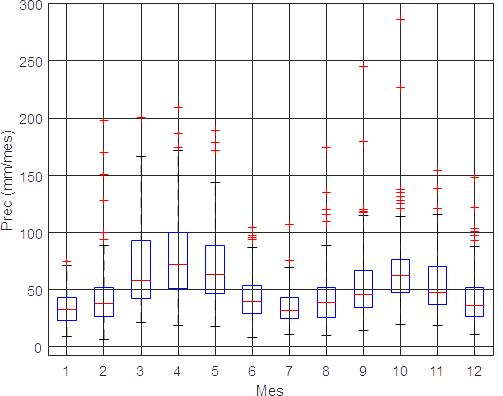
\includegraphics[height=3.in]{Figures/prec_sim.png}
%       \caption{ Valores simulados de precipitaciones mensuales en la zona de Guaslán}
%       \label{2}
%     \end{center}
%   \end{figure}


% En la figura \ref{2} se muestra a modo de ejemplo una de las series generada para una cuenca con clima costero, representativa del sector más 
% seco de la cuenca en la estación de Guaslán (cantón Riobamba). La línea roja representa el valor medio, la caja azul representa los valores situados entre los percentiles
%  25$\%$ y 75$\%$, y las barras negras los extremos (los puntos en rojo son tratados como datos atípicos). A modo de comparación,
%  en la figura \ref{3} se muestran los valores observados en la misma estación.

%  \begin{figure}[h!]
%     \begin{center}
%       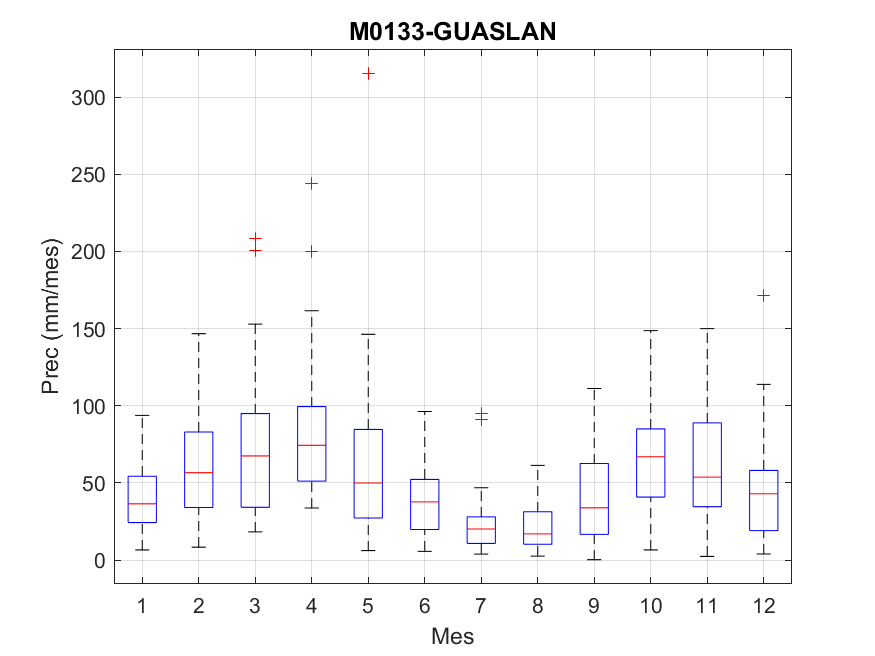
\includegraphics[height=3.in]{Figures/prec_obs.png}
%       \caption{ Valores observados de precipitaciones mensuales en la zona de Guaslán}
%       \label{3}
%     \end{center}
%   \end{figure}

%   \begin{figure}[h!]
%     \begin{center}
%       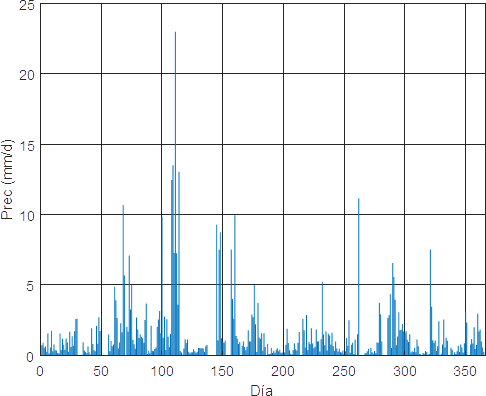
\includegraphics[height=3.in]{Figures/prec_sint.png}
%       \caption{ Un año de valores de precipitación diaria simulada en la zona de Guaslán}
%       \label{3}
%     \end{center}
%   \end{figure}


El modelo para crear las series diarias usa el método de cascadas aleatorias multiplicativas \cite{Molnar} para 
desagregar las series mensuales. El modelo consta de dos parámetros: denominados $sig2$ y $beta$
que determinan la variabilidad e intermitencia de la lluvia (proporción media de días sin lluvia) y se usan para 
ajustar el modelo, con los valores observados en las series de precipitación disponibles.


% \subsubsection{Comportamiento del régimen de precipitación}
% \label{regimenes_prec}
% Con el fin de poder realizar un estudio completo de cómo es el comportamiento del régimen de precipitaciones, 
% se seleccionaron 35 estaciones  meteorológicas que abarcan de manera uniforme el area de la cuenca de Chambo y sus alrededores.
% Se han identificado principalmente dos regímenes diferentes, un régimen bimodal en el oeste (dos períodos secos y dos de lluvias al año) 
% y el régimen monomodal (un período seco y uno de lluvias) en el este, con una franja que contiene un régimen mixto en 
% las zonas centrales de la cuenca.










\section{Series de temperatura}
\label{tempint}
Para la generación de las series de temperatura se utilizado datos de 10 termómetros situados en el entorno del área de estudio.
Estos datos han sido sometidos al un proceso de curado que por un lado define una frontera para detectar outliers o datos atípicos
siguiendo el siguiente criterio:
\begin{equation}
  si~X_i>5\cdot\sigma^2_n~es~un~utlier,~donde~\sigma^2_n=\frac{1}{n}\cdot\sum^n_{i=1}\bigg(X_i-\bar{X}\bigg)^2
\end{equation}
y por el otro lado elimina los datos que presentan un cierto grado de persistencia \cite{Estevez}
Los datos faltantes se han completados de manera similar a cómo se procedió con las series 
de precipitación utilizando los datos de ERA5.


\begin{figure}[h!]
  \begin{center}
    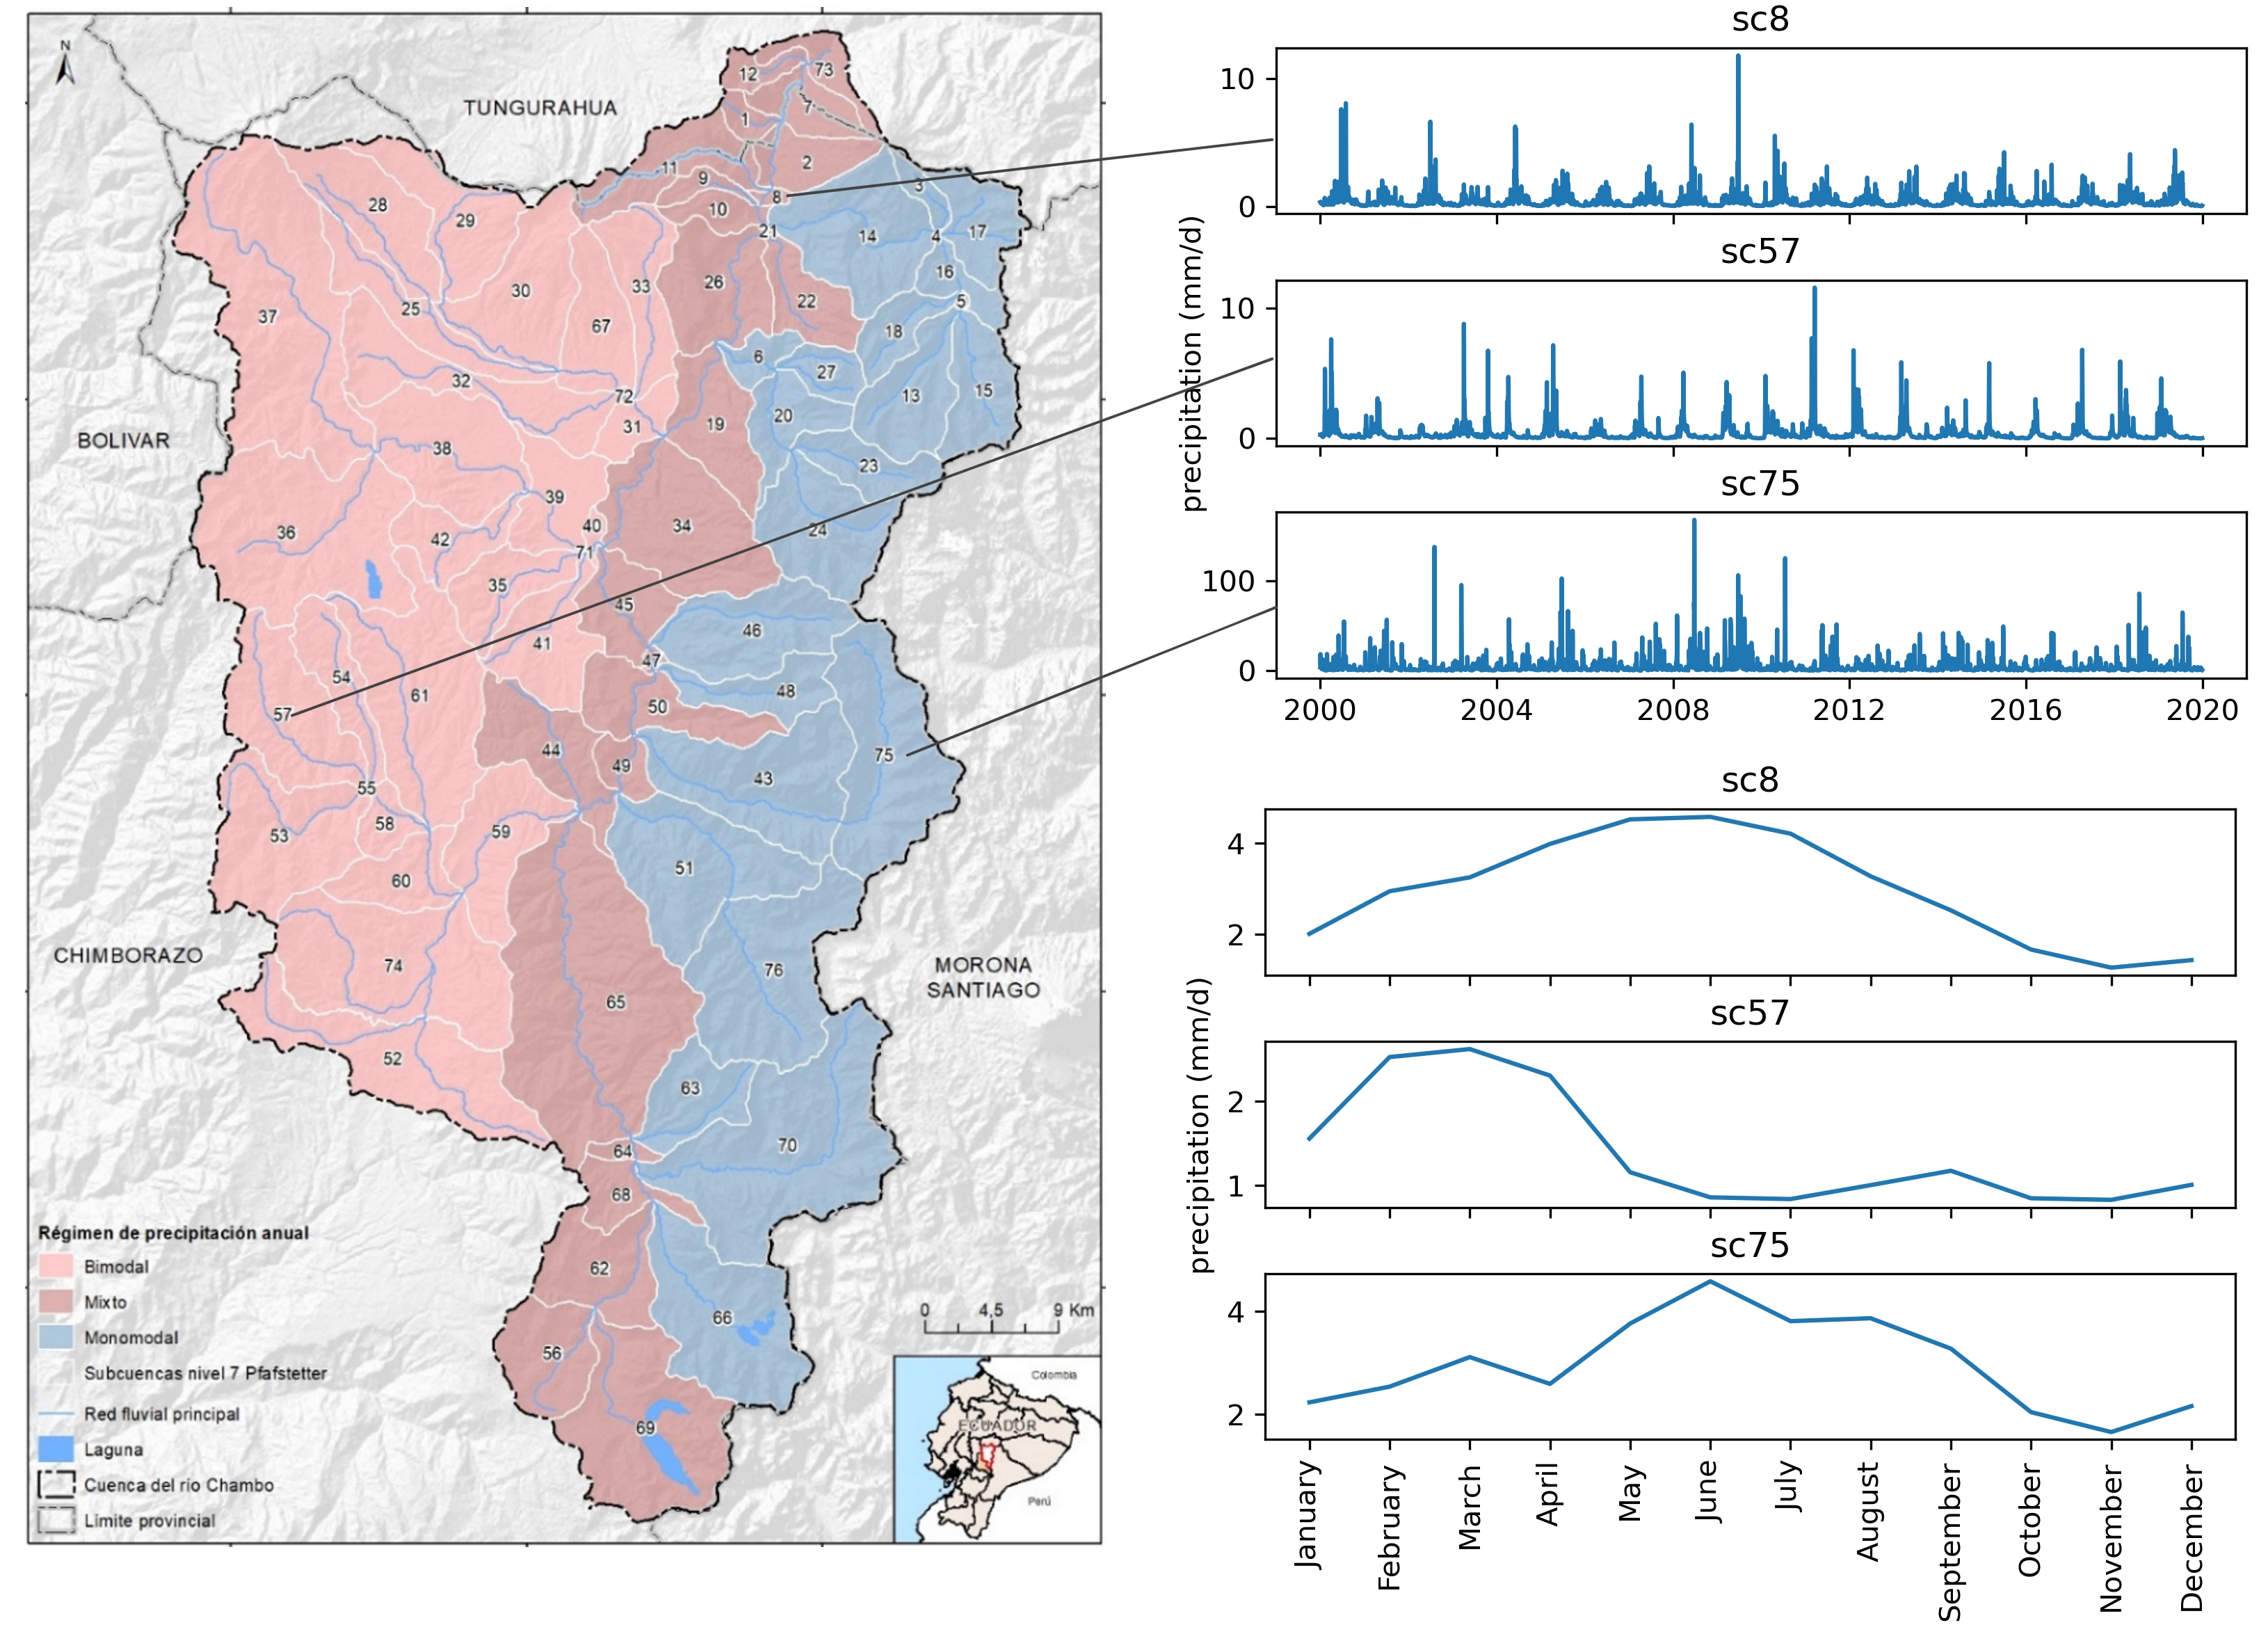
\includegraphics[height=6.5in]{Figures/cuenca_con_subcuencas_prec.png}
    \caption{ Series de precipitación para diferentes regiones de la cuenca Chambo. En los panel superior derechos se muestra la serie 
    de precipitación correspondiente al año 2019 y  los valores medios mensuales desde el año 2000 hasta el año 2020. En el panel 
    inferior, se muestran las series de temperatura máxima y mínima diarias.}
    \label{4}
  \end{center}
\end{figure}

En la figure \ref{4}, se muestran a modo de ejemplo las series de precipitación y temperaturas
mínimas y máximas generadas para tres diferentes subcuencas 
localizadas en diferentes puntos. Se puede observar las diferentes estacionalidades,
la cuenca con id = 57 presenta un  un régimen costero (donde la precipitación máxima tiene lugar en el mes de abril), 
las cuencas con ids= 8 y 75, un régimen amazónico (con un único pico de precipitación en junio-julio).



\chapter{Modelo Hidrológico}
\label{Modelo_Hidrológico}

Cómo se ha descrito anteriormente, se ha utilizado el modelo hidrológico MELCA
 para generar las series de caudales de descarga que han sido utilizadas como variables objetivos
al entrenar los modelos de redes neuronales (capítulo \ref{ANNs}). 
 Este modelo está basado en LEM y fue desarrollado por IHCantabria.
 A continuación se describen las características principales de estos modelos.

\section{Modelo LEM}

Este modelo simula el proceso hidrológico en una cuenca hidrográfica a partir de las siguientes hipótesis empíricas:
\begin{enumerate}
    \item Las cuencas hidrográficas son sistemas complejos que persiguen continuamente un equilibrio dinámico, 
    dado por una combinación de factores climáticos ( precipitación y evapotranspiración potencial) 
    y algunas características del terreno (topografía, vegetación, suelo, geología, etc.). 

    La evolución de la escorrentía ($R$) hacia el equilibrio sigue la ley clásica de crecimiento descrito por la 
    ecuación logística:

    \begin{equation}
        \frac{d R(t)}{dt}=K\cdot R(t)\cdot\big(1-\frac{R(t)}{R_{eq}}\big)
    \label{eq.log}
    \end{equation}

    \item  $Req$ es la escorrentía de equilibrio  y se puede expresar como un coeficiente de escorrentía de 
    equilibrio ($Ceq$) multiplicado por la precipitación instantánea: $Req = P \cdot Ceq$. 
    
    \item $K$ es la tasa de crecimiento y es una función lineal de la precipitación: $K=P/S_0$ , donde $S_0$ 
    es una constante con unidades de longitud ($mm$) que representa un espesor característico del suelo.
    \item La ecuación logística no considera el  tiempo de viaje desde las 
    zonas de producción de escorrentía hasta el punto final de medida del caudal, en la salida de la cuenca. 
    Cuando el intervalo de tiempo de análisis es del mismo orden de magnitud que el tiempo 
    de respuesta de una cuenca, se debe agregar un método de propagación.


\end{enumerate}

La versión estándar del LEM adopta un modelo lineal para el submodelo de enrutamiento y toma la forma del siguiente sistema 
de ecuaciones:


\begin{equation}
    \frac{d R(t)}{dt}=\frac{P(t)}{S_0}\cdot R(t)\cdot\big(1-\frac{R(t)}{R_{eq}}\big)
\end{equation}

\begin{equation}
    \frac{d \hat{P}}{dt}=P(t)-\frac{\hat{P}}{\lambda}
\end{equation}


\begin{equation}
    \frac{d \hat{E}}{dt}=E(t)-\frac{\hat{E}}{\lambda}
\end{equation}


\begin{equation}
    R_{eq}(t)=P(t)\cdot C_{eq}(\psi);\ \ C_{eq}(\psi)=e^{-a\cdot \psi}, \psi=\frac{\hat{E}}{\hat{P}}
\end{equation}


\begin{equation}
    \frac{d Q(t)}{dt}=\frac{1}{\tau}\cdot \big[R(t)-Q(t)\big]
\end{equation}


Donde $R$ y $Q$ son la escorrentía total y la descarga medida en la salida de la cuenca, respectivamente. 
$P$ y $E$ son la precipitación y la evapotranspiración potencial en cada paso de tiempo, mientras que $\hat{P}$ y $\hat{E}$ 
son valores promediados de $P$ y $E$ durante un periodo de tiempo característico, respectivamente. 
Los parámetros del modelo entonces son:
\begin{itemize}
    \item $\lambda$ (días), el tiempo característico de respuesta  de la cuenca. %($1/(25.465*log(s0)-19.494)$).
    \item $S_0$ (mm), que representa un espesor medio de suelo o una capacidad de almacenamiento característica de la cuenca.
    \item $a$, un parámetro adimensional que modifica la forma de la función de equilibrio (típicamente en el rango 0.5-1.5)
    \item $\tau$ (horas), el parámetro de enrutamiento, que puede considerarse un tiempo 
    de respuesta rápido de la cuenca.
\end{itemize}
Este sistema de ecuaciones diferenciales ordinarias puede resolverse numéricamente con un esquema explícito 
incondicionalmente estable, ya que  que todas las ecuaciones, y en especial la logística, tienen solución analítica.

Como se ha mencionado en el capítulo \ref{datos}, los datos de precipitación correspondientes a las zonas más 
altas de la cuenca son escasos. Es por esto que es necesario aplicar  dos factores $fcp$ y $fce$ 
que tienen en cuenta la influencia de la altitud de cada subcuenca y
 sirven para calibrar el modelo y corregir las series de precipitaciones y evo-transpiración, respectivamente.
 Para calibrar el modelo se han utilizado datos de caudales recogidos por diferentes estaciones de aforo proporcionados por
 MAATE \cite{MAATE} y los valores de caudal promedio aportados por el documento de ``\textit{Aportes a la planificación para 
 la gestión integral de los recursos hídricos}'' citado en \cite{Rodriguez}. 
 El modelo es entonces calibrado en cada sub-cuenca de manera individual, ajustando los factores de corrección $fcp$ y $fce$ 
 de modo tal que los caudales   mensuales medios  simulados se acerquen lo más posible a los valores medidos en las estaciones de aforo.
 
 
%  \begin{figure}[h!]
%      \begin{center}
%        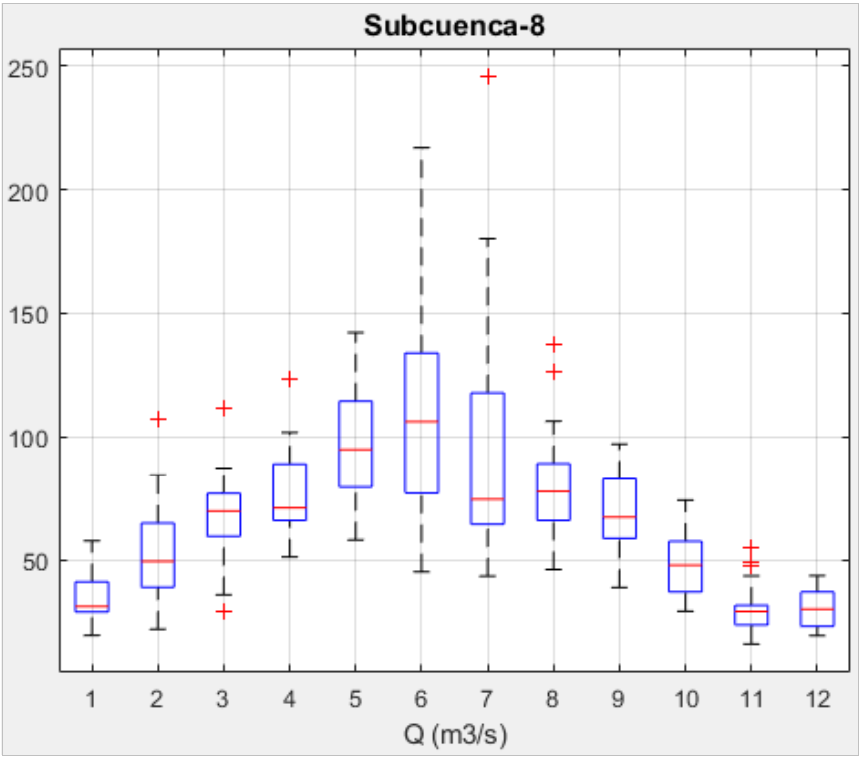
\includegraphics[height=3.in]{Figures/caudal_sim.PNG}
%        \caption{ Valores simulados de caudales mensuales para la subcuenca 8.}
%        \label{2}
%      \end{center}
%    \end{figure}
 
 
 
%   \begin{figure}[h!]
%      \begin{center}
%        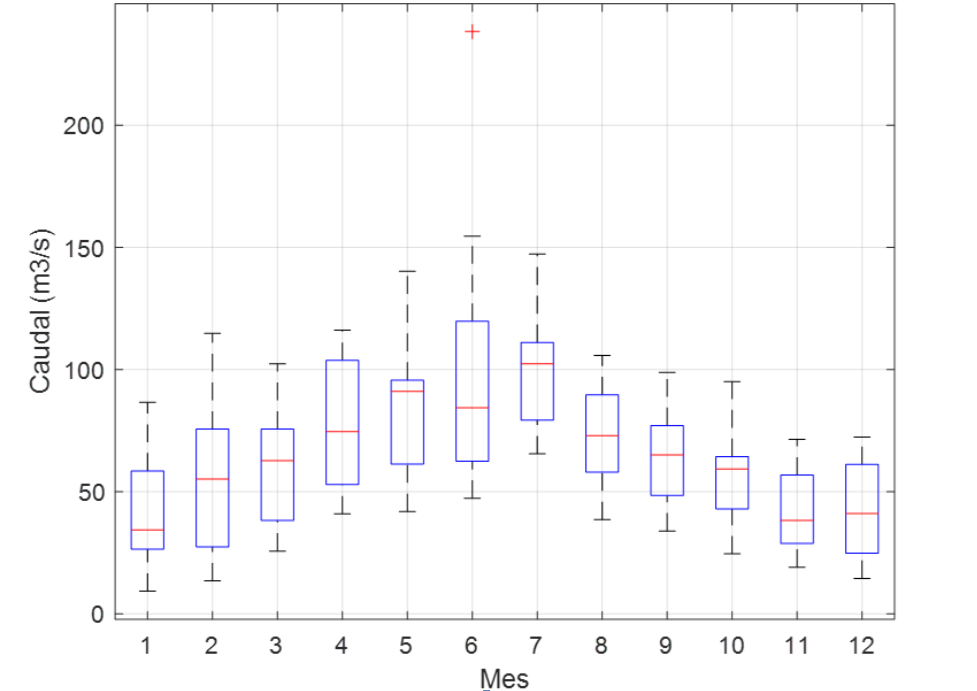
\includegraphics[height=3.in]{Figures/caudal_obs.PNG}
%        \caption{ Valores observados de caudales mensuales para la subcuenca 8.}
%        \label{3}
%      \end{center}
%    \end{figure}
 
 
 
%    En la figura \ref{2} se muestran a modo de ejemplo, los valores observados (panel inferior) y simulados  (panel superior) para la subcuenca 8.
%    La línea roja representa el valor medio, la caja azul representa los valores situados entre los percentiles
%    25$\%$ y 75$\%$, y las barras negras los extremos (los puntos en rojo son tratados como datos atípicos). 
%     Se puede observar que a calibración ha ayudado a igualar considerablemente los caudales modelados con los caudales aforados.



\subsection{Modelo MELCA}

MELCA es un modelo hidrológico semi-distribuido basado en LEM. 
Este modelo considera varias subcuencas, cada una de ellas con sus parámetros y forzamientos climáticos diferenciados
y permite incluir una serie de particularidades asociadas a las cuencas tropicales andinas como la inclusión de páramos 
y bofedales con sus topologías y el estado de conservación. El modelo convierte la superficie de cada uno de estos 
ecosistemas andinos en una capacidad equivalente de almacenamiento del suelo. 
También  incluye factores de corrección para  la evo-transpiración en zonas de alta montaña, el efecto de glaciares 
y la aportación de agua atmosférica proveniente de niebla (flujo que es significativo en zonas cuencas andinas tropicales). 


\begin{figure}[h!]
    \begin{center}
      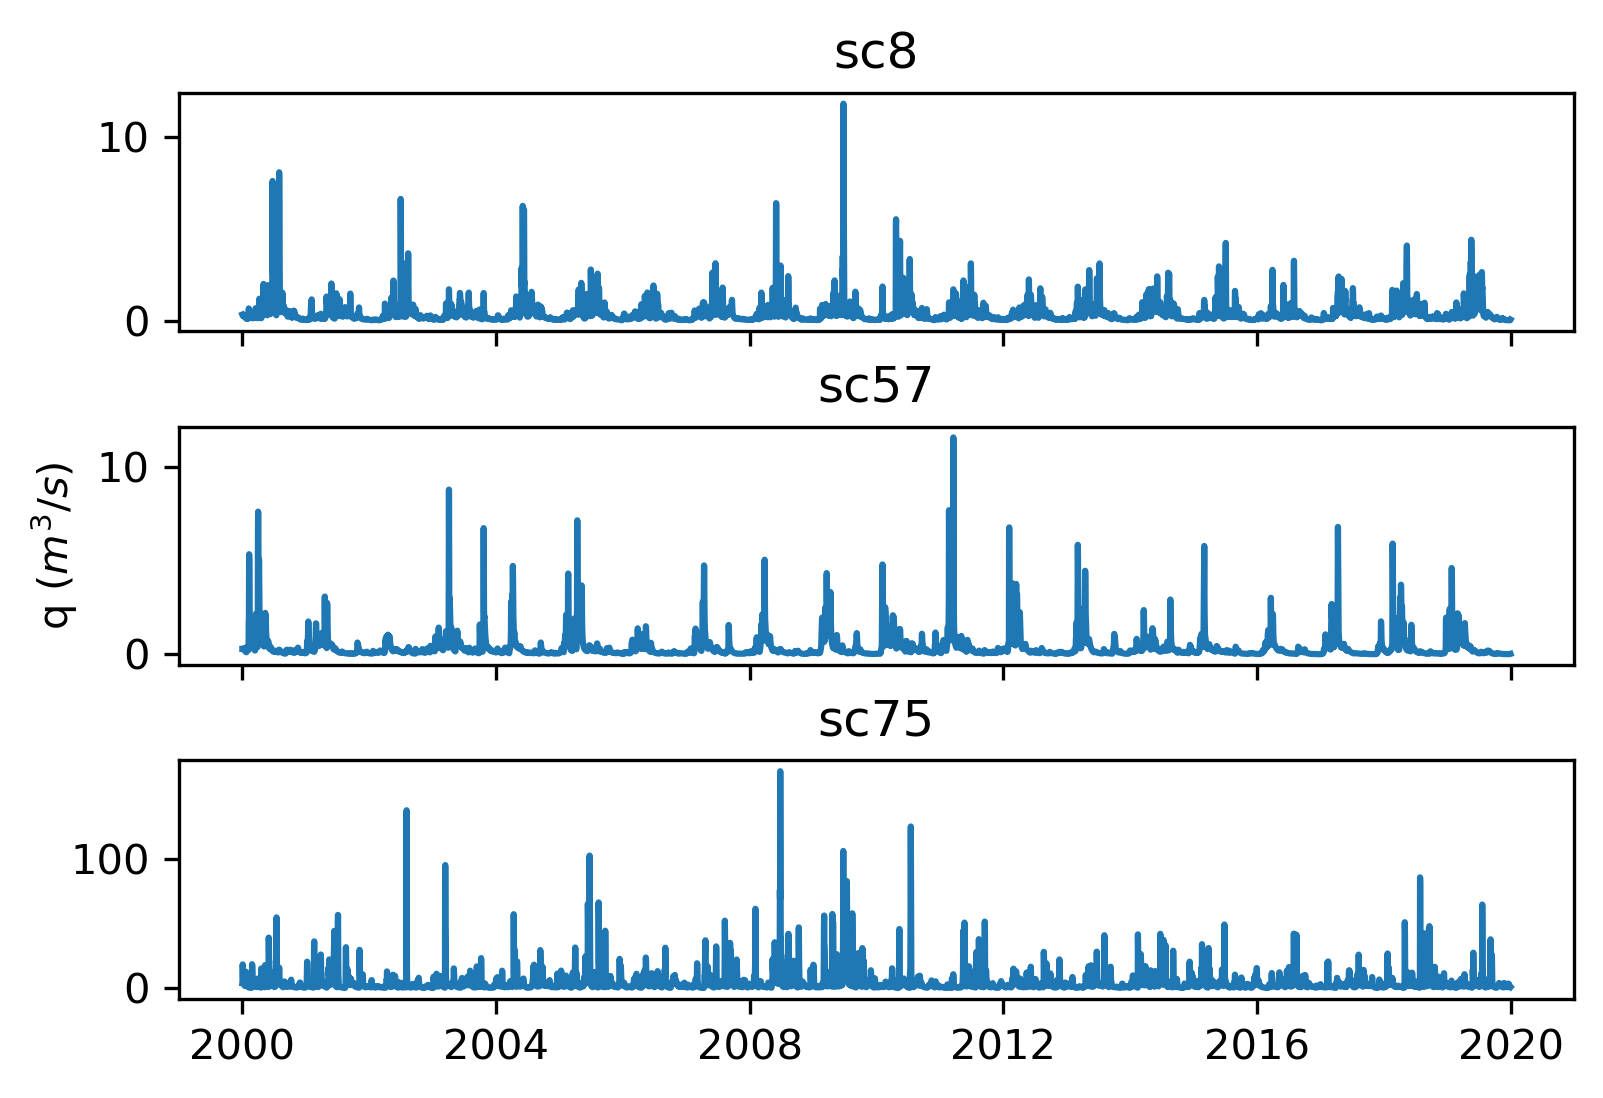
\includegraphics[height=3.5in]{Figures/caudales.png}
      \caption{ Caudales diarios simulados con el modelo MELCA para las cuencas con ids 8, 57 y 75 desde el año 2000 hasta
      el año 2020. }
      \label{caudales}
    \end{center}
  \end{figure}

En la figura \ref{caudales} se muestran a modo de ejemplo los caudales de descarga diarios simulados con el modelo MELCA 
para las cuencas con ids 8, 57 y 75. Se puede observar que la cuenca 75, que se encuentra más cerca del amazonas y con 
un régimen más húmedo, posee una caudal considerablemente mayor.
% \subsection{Parámetros físicos}
% El modelo LEM  usa 5 parámetros de entrada, el área de la cuenca, 
% el almacenamiento característico $s_0$, el parámetro de enrutamiento $\tau$, 
% el factor corrector de las precipitaciones $fcp$ y el factor corrector de la evo-transpiración $fce$. 

% \subsubsection{Capacidad de almacenamiento}
% La capacidad de almacenamiento del terreno se ha estimado mediante el método del Número de 
% Curva del \textit{Soil Conservation Service} (SCS).

% Si consideramos que para una cantidad de precipitación $P$, una cantidad $P_e$ se escurre directamente y una cantidad
% $I_a$ se infiltra inicialmente. Por otro lado, una cantidad de agua $F_a$ es retenida y es  
% menor a la capacidad máxima de almacenamiento de la cuenca $S_{max}$.

% El método SCS supone que entre todas las cantidades descriptas, se satisface la siguiente relación:
% \begin{equation}
%     \frac{F_a}{S_{max}}=\frac{P_e}{P-I_a}
% \end{equation}

% Si además aplicamos el principio de continuidad para la precipitación, $P = P_e+I_a+F_a$ y la relación experimental
% entre $S_{max}$ y $I_a$, $I_a=0,2\cdot S_max$, obtenemos una relación entre $P_e$ y $S_{max}$:

% \begin{equation}
%     P_e=\frac{(P-0,2\cdot S_{max})^2}{P-0,8\cdot S_{max}}
% \end{equation}


% El número de curva (CN) se relaciona con la capacidad de almacenamiento máxima de la cuenca de la siguiente manera:

% \begin{equation}
%     S_{max}=25,4\cdot\bigg(\frac{1000}{CN}-10\bigg)
% \end{equation}

% Los números de curva se encuentran tabulados en función del tipo y uso del suelo (referencia).

% Una vez conocidas las capacidades máximas de almacenamiento del suelo por subcuencas, podemos calcular el 
% almacenamiento característico $S_0$, tal y como lo requiere el modelo LEM, antes descrito. 
% De acuerdo a la experiencia de aplicación del modelo en otras cuencas, podemos asumir con  con buen grado de 
% ajuste la siguiente relación:

% \begin{equation}
%     S_{max}=9\cdot S0
% \end{equation}

% \subsubsection{Coeficiente de enrutamiento}

% El parámetro de enrutamiento $\tau$ representa el retardo entre la generación 
% de la escorrentía en el territorio y su llegada al punto de medida en el final de cada tramo. Este parámetro 
% tiene muy poca influencia en el cálculo de los recursos hídricos, ya que no altera el balance de masa, sino que 
% retrasa ligeramente la llegada del caudal (unas horas, mientras que el paso de tiempo de cálculo es un día). 

% \subsubsection{Factores correctores de las precipitaciones}
% Como se ha mencionado en el capítulo \ref{capitulo 1}, los datos de precipitación correspondientes a las zonas más 
% altas de la cuenca son escasos. Es por esto que es necesario aplicar un factor de corrección, $fcp$, a las series de precipitación
% que tiene en cuenta la influencia de la altitud de cada subcuenca, en general las subcuencas que se encuentran a mayor
% altitud tendrán un factor de corrección mayor. 

% \subsubsection{Cálculo de la evapotranspiración corregida}

% La evapotranspiración potencial (ETP) se ha calculado con base en la fórmula de la FAO 56 PM (referencia), 
% que toma los datos de temperatura máxima y mínima de rásteres en cada subcuenca:

% \begin{equation}
%     ETP_0\bigg(\frac{mm}{d}\bigg)=\frac{12,64}{365,25}\cdot \bigg(T_{med}+17,8\bigg)\cdot\bigg(T_{max}-T_{min}\bigg)^{0,5}
% \end{equation}

% Para calcular las temperaturas máximas y mínimas diarias, Tmax y Tmin, se han usado las interpolaciones de los datos 
% instrumentales y la base de datos de ERA5 \ref{tempint}.


% En las cuencas ecuatorianas andinas, la fórmula anterior tiende a sobreestimar la ETP en hasta un 30 $\%$ (Córdova,2015),
% ya que no considera el efecto del aumento de radiación solar ni las condiciones locales de humedad relativa y por otro lado 
% la presencia de viento en esas zonas también distorsiona el valor de ETP. Por lo tanto, se ha aplicado un factor corrector al 
% resultado de la fórmula de la FAO que depende de la altitud y orientación de cada cuenca:

% \begin{equation}
%     ETP\bigg(\frac{mm}{d}\bigg)=f_{ce}\cdot ETP_0\bigg(\frac{mm}{d}\bigg)
% \end{equation}

% \subsubsection{Calibración del modelo}



% \subsubsection{Resultados obtenidos con MELCA}



  

% \begin{figure}[h!]
%     \begin{center}
%       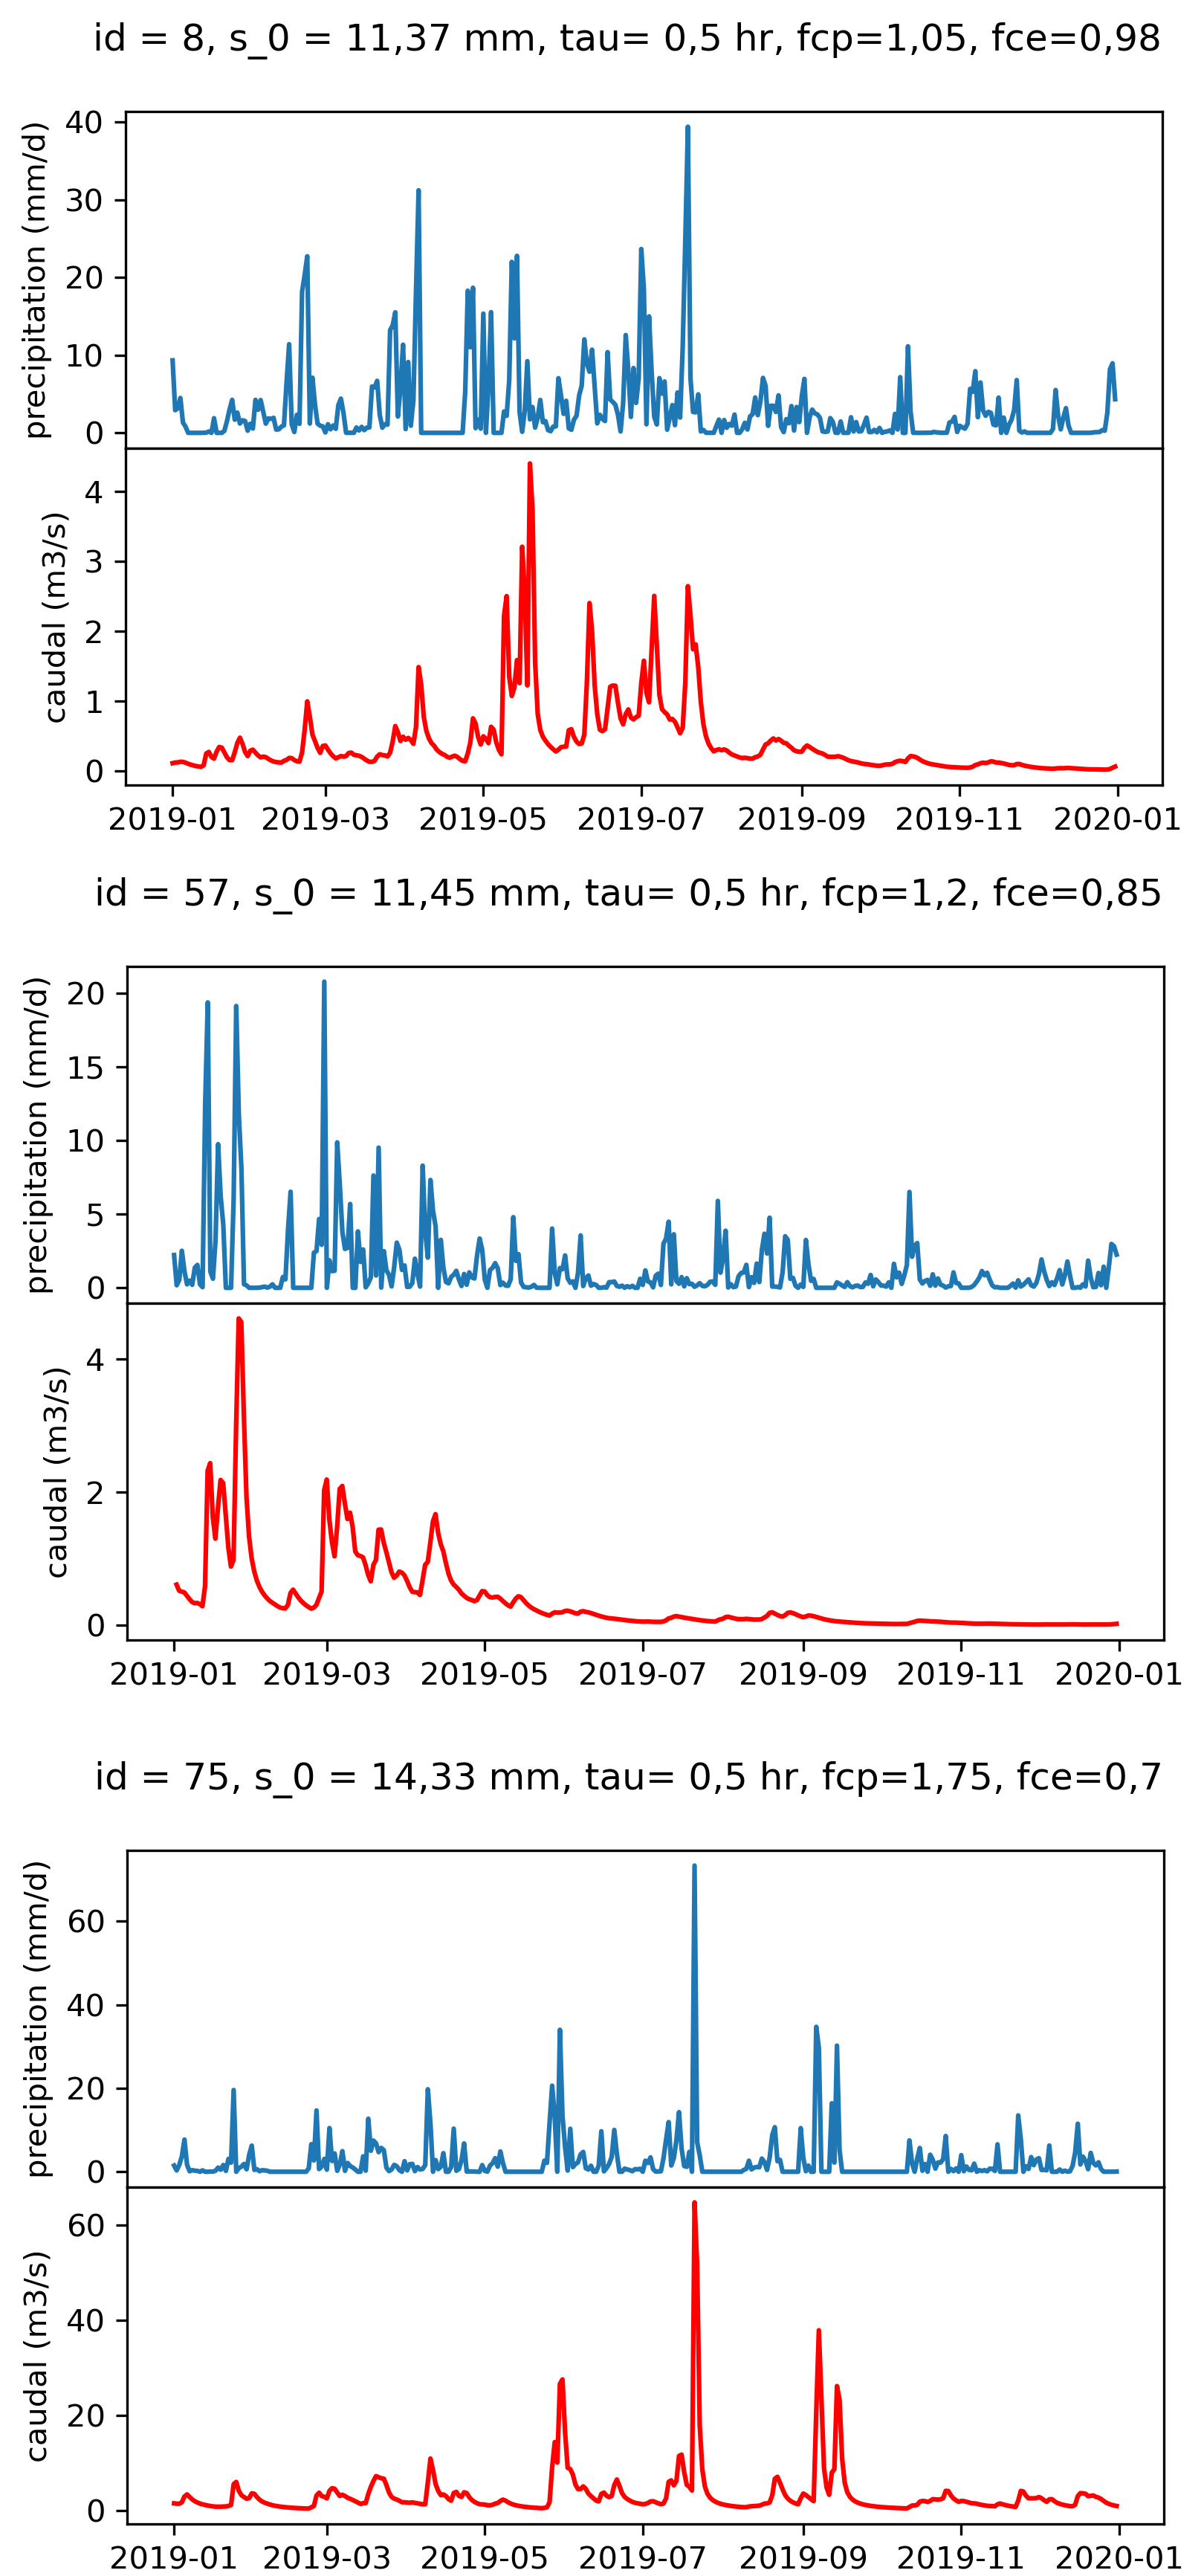
\includegraphics[height=6.5in]{Figures/outputs_MELCA.png}
%       \caption{ Simulaciones de caudales naturales para tres subcuencas durante el añ0 2019, 
%       en las graficas superiores se muestran las series de 
%       precipitación de entrada y los parámetros del modelo.}
%       \label{5}
%     \end{center}
%   \end{figure}

%   \begin{figure}[h!]
%     \begin{center}
%       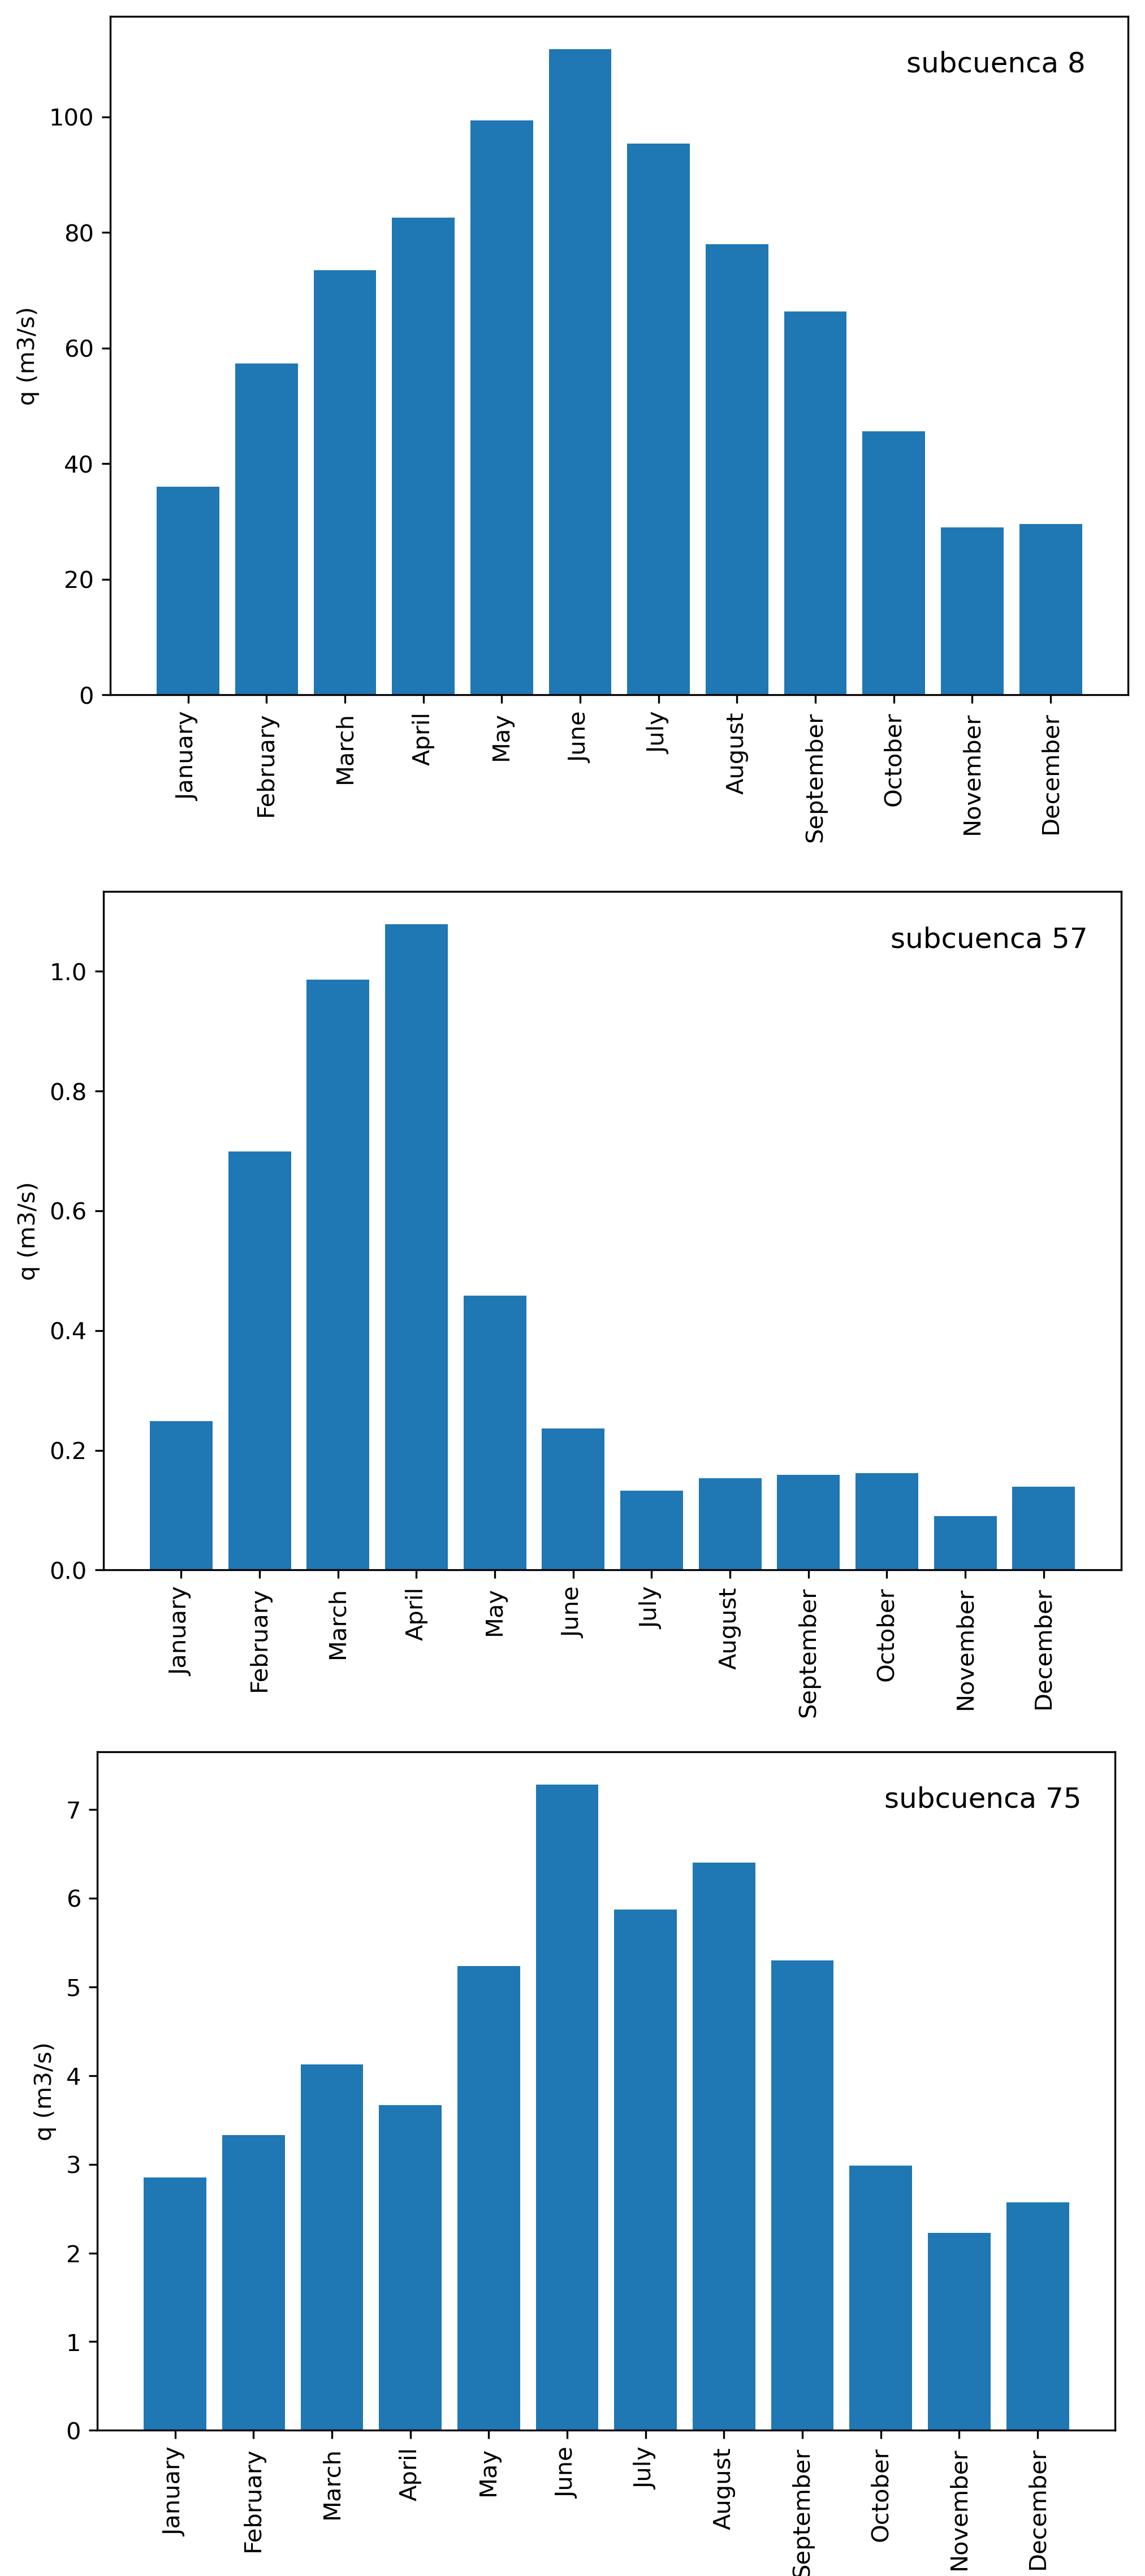
\includegraphics[height=6.5in]{Figures/outputs_MELCA_mensuales.png}
%       \caption{ Valores medios mensuales de caudal natural para tres subcuencas durante los años 2000 y 2020.}
%       \label{6}
%     \end{center}
%   \end{figure}

%  En la figura \ref{5} se muestran graficas con los resultados  para 
% las subcuencas con id 8, 57 y 75 (ver figura \ref{4}). 
% En los paneles superiores se muestras las series de precipitación de entrada y los parámetros del modelo, 
% capacidad de almacenamiento,
% coeficiente de enrutamiento y los factores de corrección. 
% La cuenca más alta es la 75 (?) y posee el mayor factor de corrección fcp,
% la más baja es la 8 y tiene el factor de corrección menor.

% Tal y como vimos en la sección \ref{regimenes_prec}, la subcuenca 8 presenta un regimen de precipitaciones 
% mixto, de las tres cuencas es la que se encuentra más aguas abajo por lo que el caudal medio, ---, es 
% considerablemente superior que en las otras dos. Su area es de --
% la superficie agregada de la cuenca es de --- 
% (sumando la superficie de las cuencas aguas arriba que vierten ella) lo que se produce en una productividad de ---.
% La cuenca 57 se encuentra en la region oeste, presente un regimen bimodal, caudal medio de ---, superficie --- y 
% productividad media de ---, mientras que la cuenca 75 presenta un régimen monomodal y sus valores son---, ---
% y respectivamente.



% En la figura ... se muestran los caudales medios mensuales
% para la salida de la cuenca (subcuenca 73) . El caudal medio es de --- $m^3/s$ 
% este asciende a un valor máximo de ...entre los meses de ... y de ...., y presenta un mínimo de .... entre los meses de ....
% y ..... La superficie agregada de la cuenca es de 3590 $km^2$, con una precipitación media de 1120 $mm$ que se traducen en una 
% productividad de ----.

  

% \subsection{Parámetros físicos}
% \subsubsection{Capacidad máxima de almacenamiento del terreno}

% Las ecuaciones anteriores pueden aplicarse de manera agregada para toda una cuenca, considerada como un ente único, 
% o bien de manera semi-distribuida, considerando varias subcuencas, cada una de ellas con sus parámetros y forzamientos 
% climáticos diferenciados. Si se emplea el modelo en un marco semi-distribuido, es preciso incluir, cuando el paso temporal
%  de cálculo lo requiera, la traslación del flujo desde cada subcuenca al punto de salida. El MELCA es precisamente una 
%  versión semi-distribuida del LEM genérico,
%  con una serie de particularidades que se describen a continuación.

\section{Modelo MODSIM}
\label{Modelo_balance}

Una vez obtenidos los caudales para cada una de las cuencas, ya sea simulados por el modelo LEM o generados por 
los modelos de redes neuronales, se ha determinado el balance hidrológico de la cuenca mediante la utilización 
del software MODSIM \cite{modsim}, mundialmente aceptado y  empleado para simular operaciones en sistemas 
hidrológicos como soporte de decisiones. Este modelo permite incorporar simultáneamente la complejidad física, 
hidrológica y las aspectos institucionales y administrativos del manejo de una cuenca, incluyendo los derechos 
del agua. Además, brinda soporte para la toma de decisión en el uso del agua entre la agricultura, uso poblacional,
 industrial, energético y ambiental.


\begin{figure}[h!]
    \begin{center}
      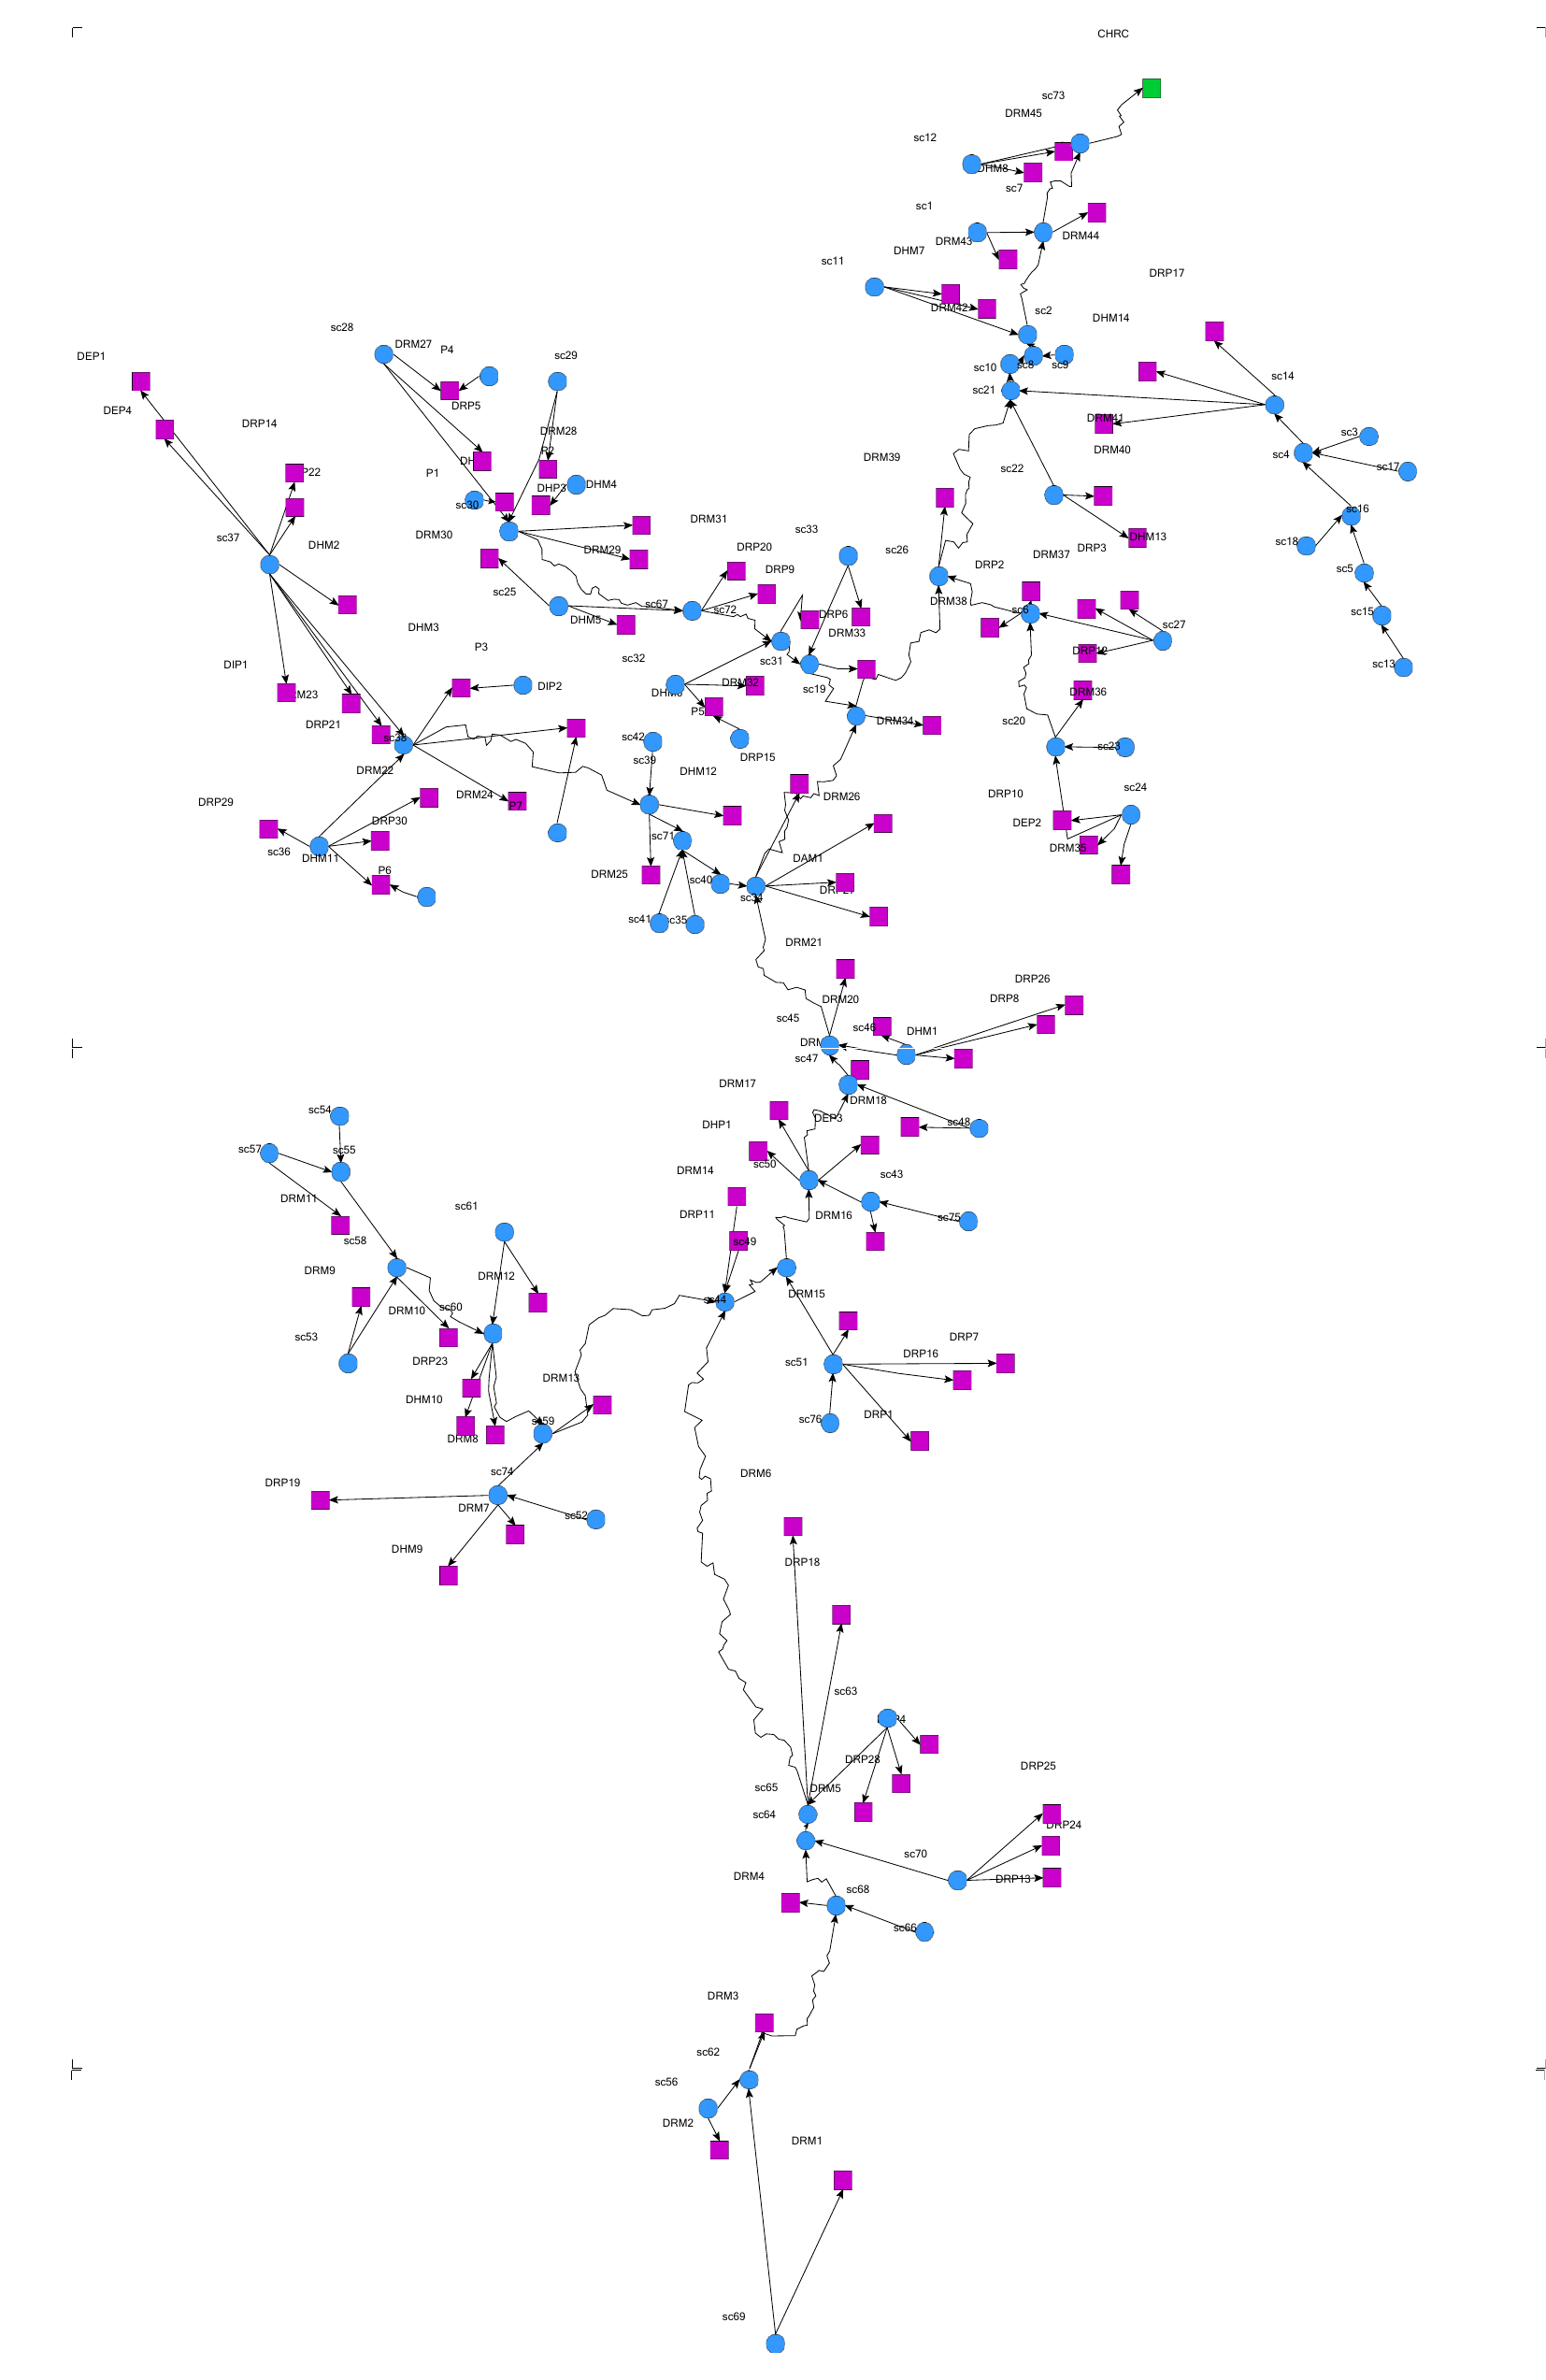
\includegraphics[height=8.5in]{Figures/modzim/figs.png}
      \caption{ Esquema conceptual de CHRC con MODSIM}
      \label{caudales}
    \end{center}
  \end{figure}

  MODSIM es un modelo compuesto por nodos y enlaces que representa el sistema que constituye una cuenca fluvial. 
  Los objetos utilizados en el modelo tienen asociados un costo, representado por un número de prioridad relativo. 
  Los nodos con número de prioridad bajo tendrán menos costo y serán satisfechos antes que los nodos con una prioridad
  mayor. Los objetos en MODSIM no se limitan a representar características físicas e hidrológicas de una cuenca 
  fluvial, sino que también se utilizan para simbolizar elementos artificiales y conceptuales para modelar mecanismos
   administrativos y legales complejos que rigen la asignación de agua. 

   Para optimizar la distribución de agua en las redes del cauce, MODSIM minimiza 
   una función objetivo definida de la siguiente forma \cite{modsim2}:

   \begin{equation}
    \sum_{k \in A}c_k\cdot q_k
   \end{equation}

   donde $q_k$ es el caudal en el enlace $k$, $c_k$ son pesos o las prioridades de derecho de agua por unidad de caudal en
   el enlace $k$. 

   La minimización de esta función debe conservar el balance de masa, es decir, 
   \begin{equation}
    \sum_{k \in O_i} q_k- \sum_{j \in I_i} q_j = b_{it}(q)
   \end{equation}

   \begin{equation}
    l_{kt} < q_k< u_{kt}
   \end{equation}

   donde $O_i$/$I_i$ es el conjunto de todos los enlaces que se originan/terminan en el nodo $i$,  
    y $b_{it}(q)$  es la ganancia o la pérdida en el nodo $i$ en el tiempo $t$. $l_{kt}$ $u_{kt}$ son los
    límites inferior y superior superior especificados, respectivamente, en el flujo en el enlace k en el tiempo t.

MODSIM es capaz tener en cuenta en el cálculo la evaporación, los flujos de retorno de las aguas subterráneas, 
las pérdidas en los canales y los requisitos de flujo en la corriente y resuelve las ecuaciones antes descriptas
con el algoritmo de relajación Lagrangiana RELAX-IV \cite{modim3}.


En la figura \ref{modsim}, se muestra el esquema conceptual que representa a la cuenca CHRC. Los círculos son
nodos sin almacenamiento que representan confluencias y desviaciones de los caudales de la cuenca,
las flechas o links representan los caudales fluyentes entre nodos y los cuadrados las demandas consuntivas de agua.
Se han considerado 4 tipos de demandas diferente: humana con prioridad 1, industrial, riego 
y acuicultura con prioridad 2 y energéticas con prioridad 3.


% Una vez obtenidos los caudales naturales y las demandas en la cuenca del río chambo se pueden calcular los caudales intervenidos
% fluyentes por los tramos de ríos. Para un primer análisis se ha creado un software que calcula para cada una de las subcuencas
% el resultado final de forma agregada teniendo en cuenta los flujos de entrada proveniente de las subcuencas aguas arriba, 
% el flujo del caudal natural local, las demandas de agua en dicha subcuenca y  el caudal de retorno de las demandas que vierten a ese tramo.
% Cabe destacar que para este primer análisis no se han establecido criterios de prioridades de las demandas por lo cual 
% no nos centraremos en un problema de optimización, en cambio consideraremos que todas las demandas tienen las mismas 
% prioridades.

% \begin{equation}
%     q_{total} = q_{entrada}+q_{natural}-q_{demandas}+q_{retornos}
%     \label{caudal_tot}
% \end{equation}

% \begin{figure}[h!]
%     \begin{center}
%       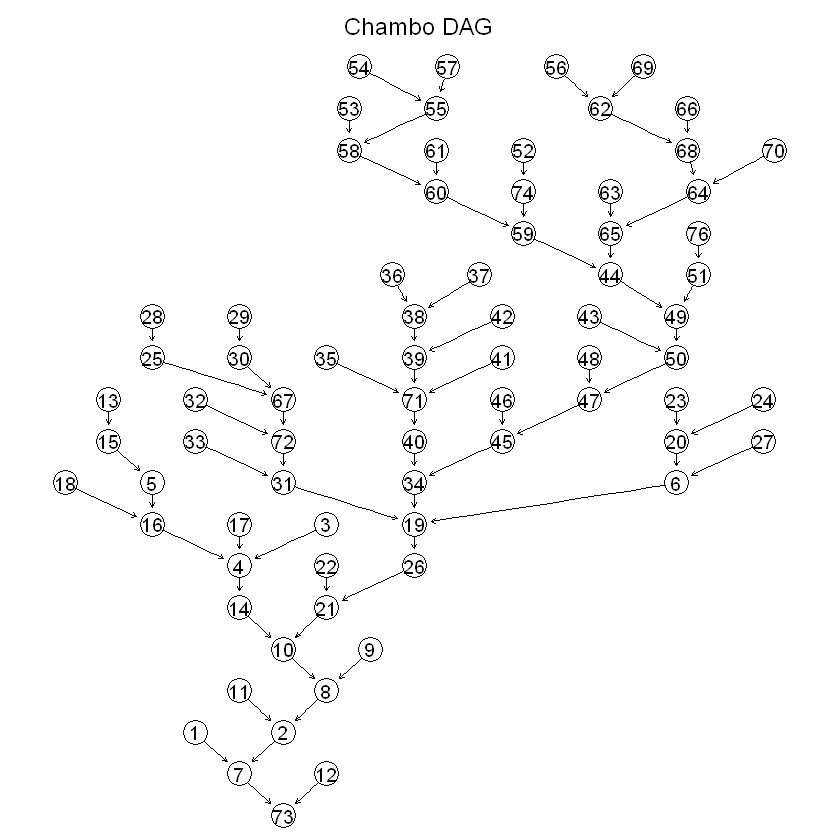
\includegraphics[height=5.in]{Figures/modelo_conceptual_cuenca.png}
%       \caption{Modelo conceptual del entramado de los tramos de la cuenca del río Chambo.}
%       \label{6}
%     \end{center}
%   \end{figure}

% En la figura \ref{6} se muestra una representación conceptual de la cuenca, donde se puede seguir el recorrido de los 
% flujos de aguay la estructura lógica que conecta las diferentes subcuencas y usos de agua. Y en la figura \ref{7} se muestra el 
% diagrama de flujos del programa que calcula el balance hidrológico para cada subcuenca. Este programa realizado en python, 
% realiza las siguientes acciones:

% \begin{enumerate}
%     \item ejecuta el modelo MELCA, cuyo resultado son las series con los caudales para todas las subcuencas de Chambo y selecciona
%     la serie correspondiente al id de la subcuenca de estudio.
%     \item utilizando la matriz de conectividades, cuyas filas  son las cuencas receptoras y cuyas columnas las cuencas 
%     tributarias (ver figura ...) encuentra los ids de las cuencas tributarias.
%     \item encuentra para cada uno de estos ids las demandas totales, seleccionando las filas que satisfacen la condiciones
%     INIC=id (ver tabla demandas) y las agrega. 
%     \item de manera similar calcula los retornos totales, pero esta vez aplicando la condición  FIN=id sobre la tabla demandas 
%     ya que los caudales de retorno son los flujos vertidos aguas abajo por las demandas
%     \item Encuentra las demandas ecosistémicas para cada uno de estos ids y las agrega.
%     \item calcula el resultado final  como en la ecuación \ref{caudal_tot}.
% \end{enumerate}


% A modo de ejemplo, si queremos calcular el caudal resultante para la sub cuenca 68, entonces las cuencas tributarias son las 66 y 62
% (ver figura \ref{6}), estas se obtienen al imponer la condición a la matriz de conectividades, $matcon[66,:]==1$. Una vez se obtienen
% los ids de las cuencas tributarias, se procede a calcular el caudal final como se explica en los puntos 3-6.


% \begin{figure}[h!]
%     \begin{center}
%       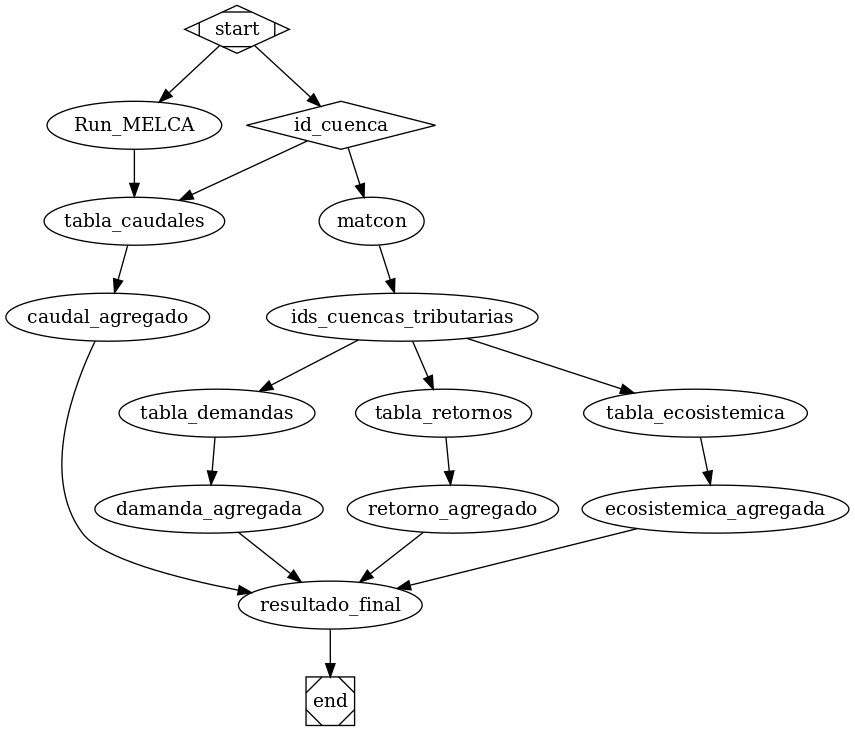
\includegraphics[height=5.in]{Figures/graphviz.png}
%       \caption{Diagrama de flujos del programa que calcula el balance hidrológico de la cuenca.}
%       \label{7}
%     \end{center}
%   \end{figure}

% \section{Modzin}

% Formato de código desde un archivo.

% \vspace{0.7cm}
% \lstinputlisting[style=codigo,language=bash,caption=ejemplo1.sh]{codigo_fuente/ejemplo1.sh}
% \vspace{0.7cm}

% Otro formato de código, para utilizar como salida de ejecución.

% \vspace{0.7cm}
% \begin{lstlisting}[style=terminal,caption=Salida del ejemplo1.sh]
% $ ./ejemplo1.sh 
% 1
% 2
% 3
% 4
% 5
% 6
% 7
% 8
% 9
% 10
% \end{lstlisting}
% \vspace{0.7cm}
\chapter{Modelos de aprendizaje profundo}
\label{ANNs}

%\section{Teoría sobre redes neuronales}
%\section{Estructura de las redes}
% He considerado tres modelos diferentes de redes neuronales: 
% \begin{itemize}
%     \item Modelo denso: Consta de dos capas densas (Fig. \ref{Red_densa})
%     \item Modelo LSTM1: Consta de una capa compuesta por una red recurrente con memoria (LSTM) y una capa densa 
%     \item Modelo LSTM2: Dos capas LSTM y una capa densa
% \end{itemize}
\section{Introducción teórica}

Las redes neuronales son modelos computacionales cuyo funcionamiento se inspira en el funcionamiento de las 
neurona cerebrales reales, su función principal es recibir, procesar y transmitir información a través de señales
químicas y eléctricas. En líneas generales, las neuronas se especializan en la recepción de estímulos y generación
de impulsos entre ellas mediante conexiones llamadas sinapsis. Cuando una neurona recibe un impulso 
eléctrico que la activa, esta dispara un impulso que a su vez estimula a otras neuronas a las que está conectada. 
Algunas de estas neuronas a su vez se activan y se disparan activando a otras y así sucesivamente 
propagando los estímulos por toda la red. Entre más se practique una tarea, las conexiones se hacen más robustas, 
esto es el proceso de aprendizaje. 

\begin{figure}[h!]
    \begin{center}
      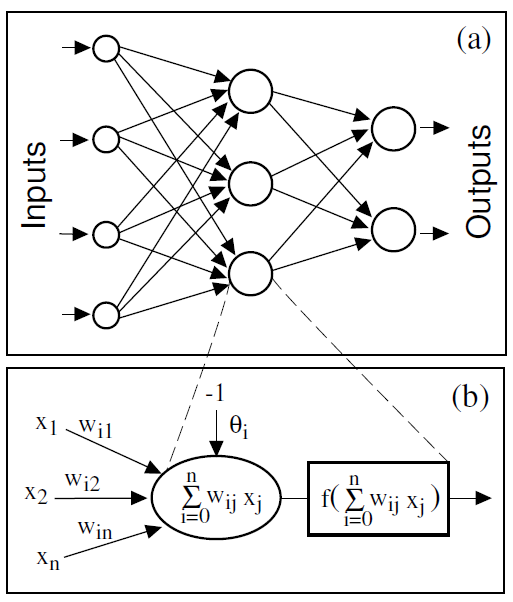
\includegraphics[height=2.5in]{Figures/esquema_red.PNG}
      \caption{ Representación gráfica de una neurona artificial (figura tomada de \cite{gutierrez}). }
      \label{perceptron}
    \end{center}
  \end{figure}

Una neurona artificial (Fig. \ref{perceptron}-b) funciona de una manera muy similar a las neuronas biológicas, 
ésta recibe datos de entrada que son combinados por la neurona asignando pesos a cada uno de ellos, a los 
cuales se aplica una función de activación que activa a la neurona si esta supera un umbral 
dado. La función de activación además de cumplir la función de activar a las neuronas, capta las 
características no lineales de los datos. 

Una red neuronal (ANNs, de sus siglas en inglés) consiste de un conjunto de neuronas conectadas entre sí 
(Fig. \ref{perceptron}-a), que al igual que en el caso de las neuronas reales son capaces de ser entrenadas para aprender 
a realizar una tarea dada generando diferentes conexiones entre ellas. 

\begin{figure}[h!]
    \begin{center}
      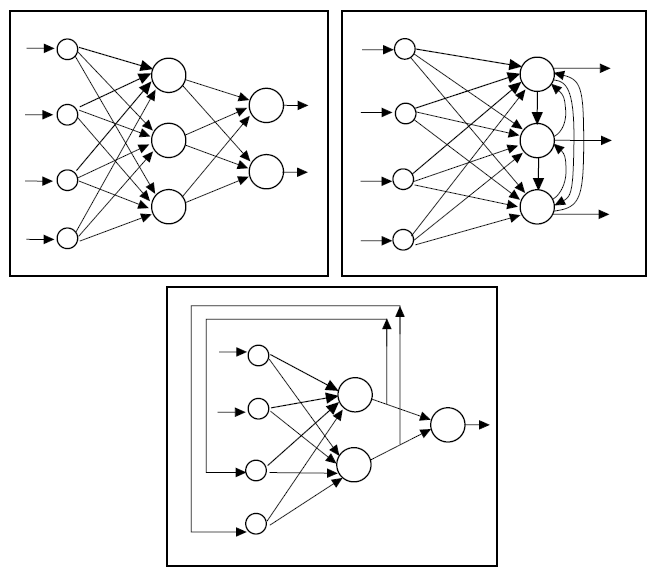
\includegraphics[height=2.5in]{Figures/topologias.PNG}
      \caption{ Tres topologías distintas de red neuronal: (a) multicapa, (b) competitivas, (c) recurrentes. }
      \label{topologias}
    \end{center}
  \end{figure}

La estructura de la red puede tener distintas topologías, en la figura \ref{topologias} se muestran tres modelos de red neuronales 
distintos: \textit{red multicapa} que solo tiene conexiones entre neuronas de capas consecutivas, 
\textit{red competitiva} que también posee conexiones entre las neuronas de la última capa y \textit{redes recurrentes} (RNN) que poseen conexiones entre 
capas no consecutivas. En este trabajo se han utilizado tanto redes multicapa como redes recurrentes, que son apropiadas para problemas de 
aprendizaje supervisado en donde cada patron de entrenamiento (entrada de la red) $X_p=(x_{1p},...x_{mp})$ tiene asociado un 
correspondiente patrón de salida $Y_p=(y_{1p},...y_{np})$. 
El entrenamiento  se basa en que la red sea capaz de reproducir los patrones de salida con el menor error posible.

El proceso de aprendizaje de la red consiste en la aplicación de métodos de optimización matemáticos para obtener los pesos $w_{ij}$ 
que minimizan una cierta función de coste o \textit{loss}. Los algoritmos más populares se basan en minimizar el error cuadrático 
medio (RMSE):

\begin{equation}
    E(w) = \sum_{j,p}(y_{jp}-\hat{y}_{jp})^2
\end{equation}

Uno de los algoritmos más simples es el de descenso de gradiente que en cada etapa intenta modificar los pesos de forma incremental de manera 
de minimizar la función de loss. El incremento de los pesos se obtiene en base al vector opuesto al gradiente del loss,
 que indica la dirección en la que la función decrece más rápidamente:

 \begin{equation}
    \Delta w_ij = -\alpha \frac{\partial E(w)}{\partial w_ij}
\end{equation}

donde $\alpha$ es la tasa de aprendizaje. 


\begin{figure}[h!]
    \begin{center}
      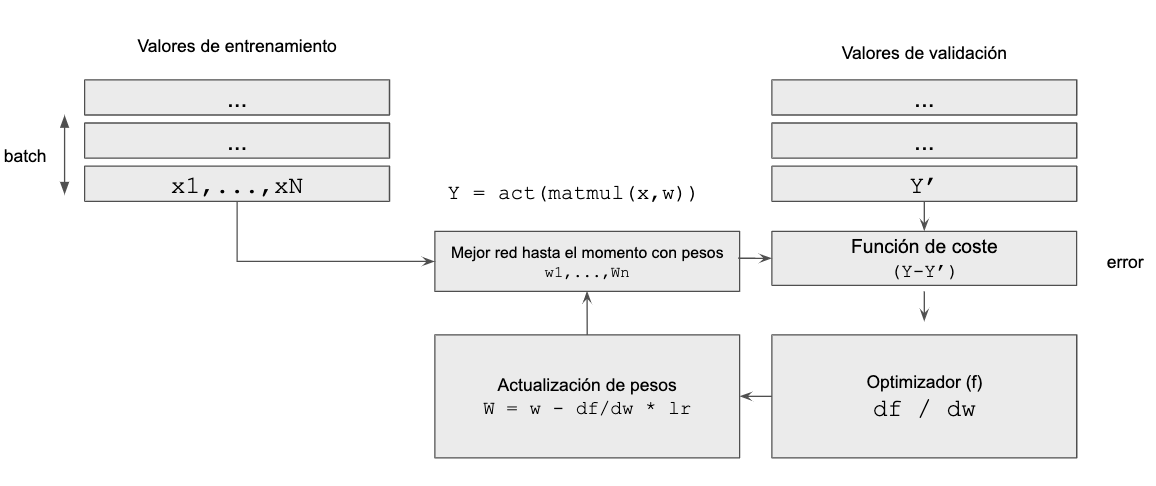
\includegraphics[height=2.in]{Figures/back_prop.png}
      \caption{ Back propagation }
      \label{backprop}
    \end{center}
  \end{figure}


El algoritmo de retro-propagación consta de dos pasos, en primer lugar la entrada $X_p$ se propaga hacia adelante, obteniendo el valor
de todas las unidades ocultas y las salidas $\hat{y}_p$ y por lo tanto el error asociado a éstas. Los valores obtenidos se utilizan para actualizar
los pesos de la capa de salida, y éstos se propagan hacia atrás para actualizar los pesos de las capas ocultas. Esto
 se repite para cada patrón de entrenamiento. En el esquema \ref{backprop} se resume todo el proceso.


% Las redes neuronales aprenden a partir de muestras o ejemplos, hacen una operación de propagación hacia adelante,
% calculan la diferencia entre sus respuestas y las respuestas correctas, y corrigen sus parámetos internos (pesos, bias) 
% según esos errores, a través de retropropagación por descenso de gradiente, o algún otro algoritmo de minimización.

% El problema es que la retropropagación es un cálculo "costoso", porque los gradientes de un nodo de cualquier capa intermedia, reciben contribuciones de muchos otros nodos de las capas anteriores. Por eso, corregir cientos o miles de parámetros con cada nuevo ejemplo, hace muy lenta la ejecución.
% Una alternativa es agrupar las muestras en "paquetes" o batches. El error se calcula sobre cada batch como la suma o promedio de errores de sus muestras, y los parámetros se corrigen una sola vez según el error del batch.
% Cuando el tamaño del batch (batch size) es igual a 1, no hay paquetes. Esto se conoce como descenso de gradiente estocástico.
% Cuando el tamaño del batch es mayor que 1 y menor que el total de muestras, se llama Descenso de Gradiente por Mini-batch.
% Cuando todas las muestras forman un sólo batch, se llama Descenso de gradiente por Batch.
\section{Redes recurrentes con memoria a largo plazo}


\begin{figure}[h!]
  \begin{center}
    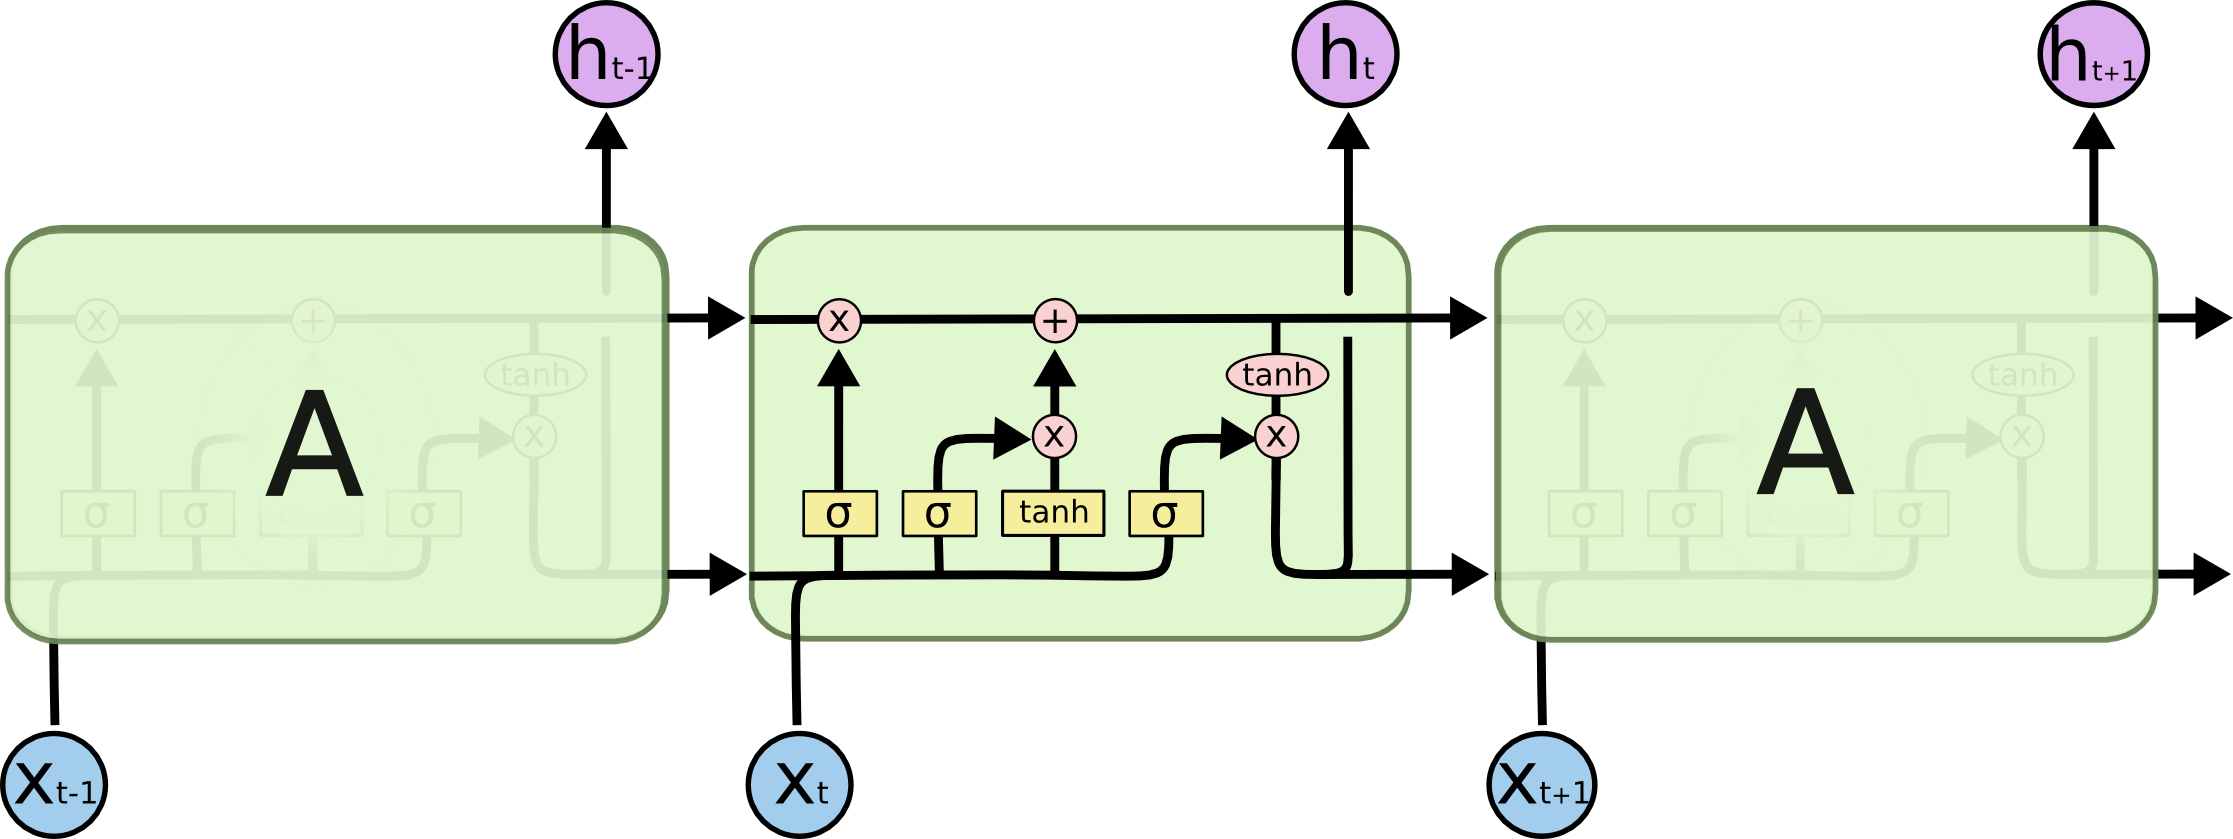
\includegraphics[height=1.8in]{Figures/LSTM3-chain.png}
    \caption{ Red neuronal recurrente con memoria a largo y corto plazo (LSTM). Figura tomada de \cite{olah}. }
    \label{LSTM}
  \end{center}
\end{figure}

Las RNNs con memoria a largo plazo (LSTM) son redes que poseen conexiones entre capas 
no consecutivas (Fig. \ref{topologias}-c) que además incluyen una conexión extra entre las neuronas dedicadas
 a almacenar información para largo períodos de tiempo. 
 Esta ``memoria a largo'' plazo soluciona el problema del desvanecimiento del gradiente que presentan las redes recurrentes 
 tradicionales\cite{Kratzert}, \cite{olah}.

En la figura \ref{LSTM} se puede observar la estructura de una celda de una red LSTM, donde $x_t$ es un input 
dado a un tiempo $t$, $h_t$ el correspondiente output, las celdas amarillas son 
capas de neuronas densas y los círculos rosas son puntos en donde se realiza una cierta operación. La clave en estas
redes es la línea horizontal superior que recorre la cadena casi sin sufrir modificaciones y permite que la información
fluya a través de la red. Mediante las cuatro entradas (celdas amarillas en el esquema),
estas redes poseen la habilidad de eliminar o agregar información al estado de la celda y decidir qué parte de la información
proveniente de capas anteriores es relevante y que parte debe ser olvidada \cite{olah}. 

\begin{figure}[h!]
  \begin{center}
    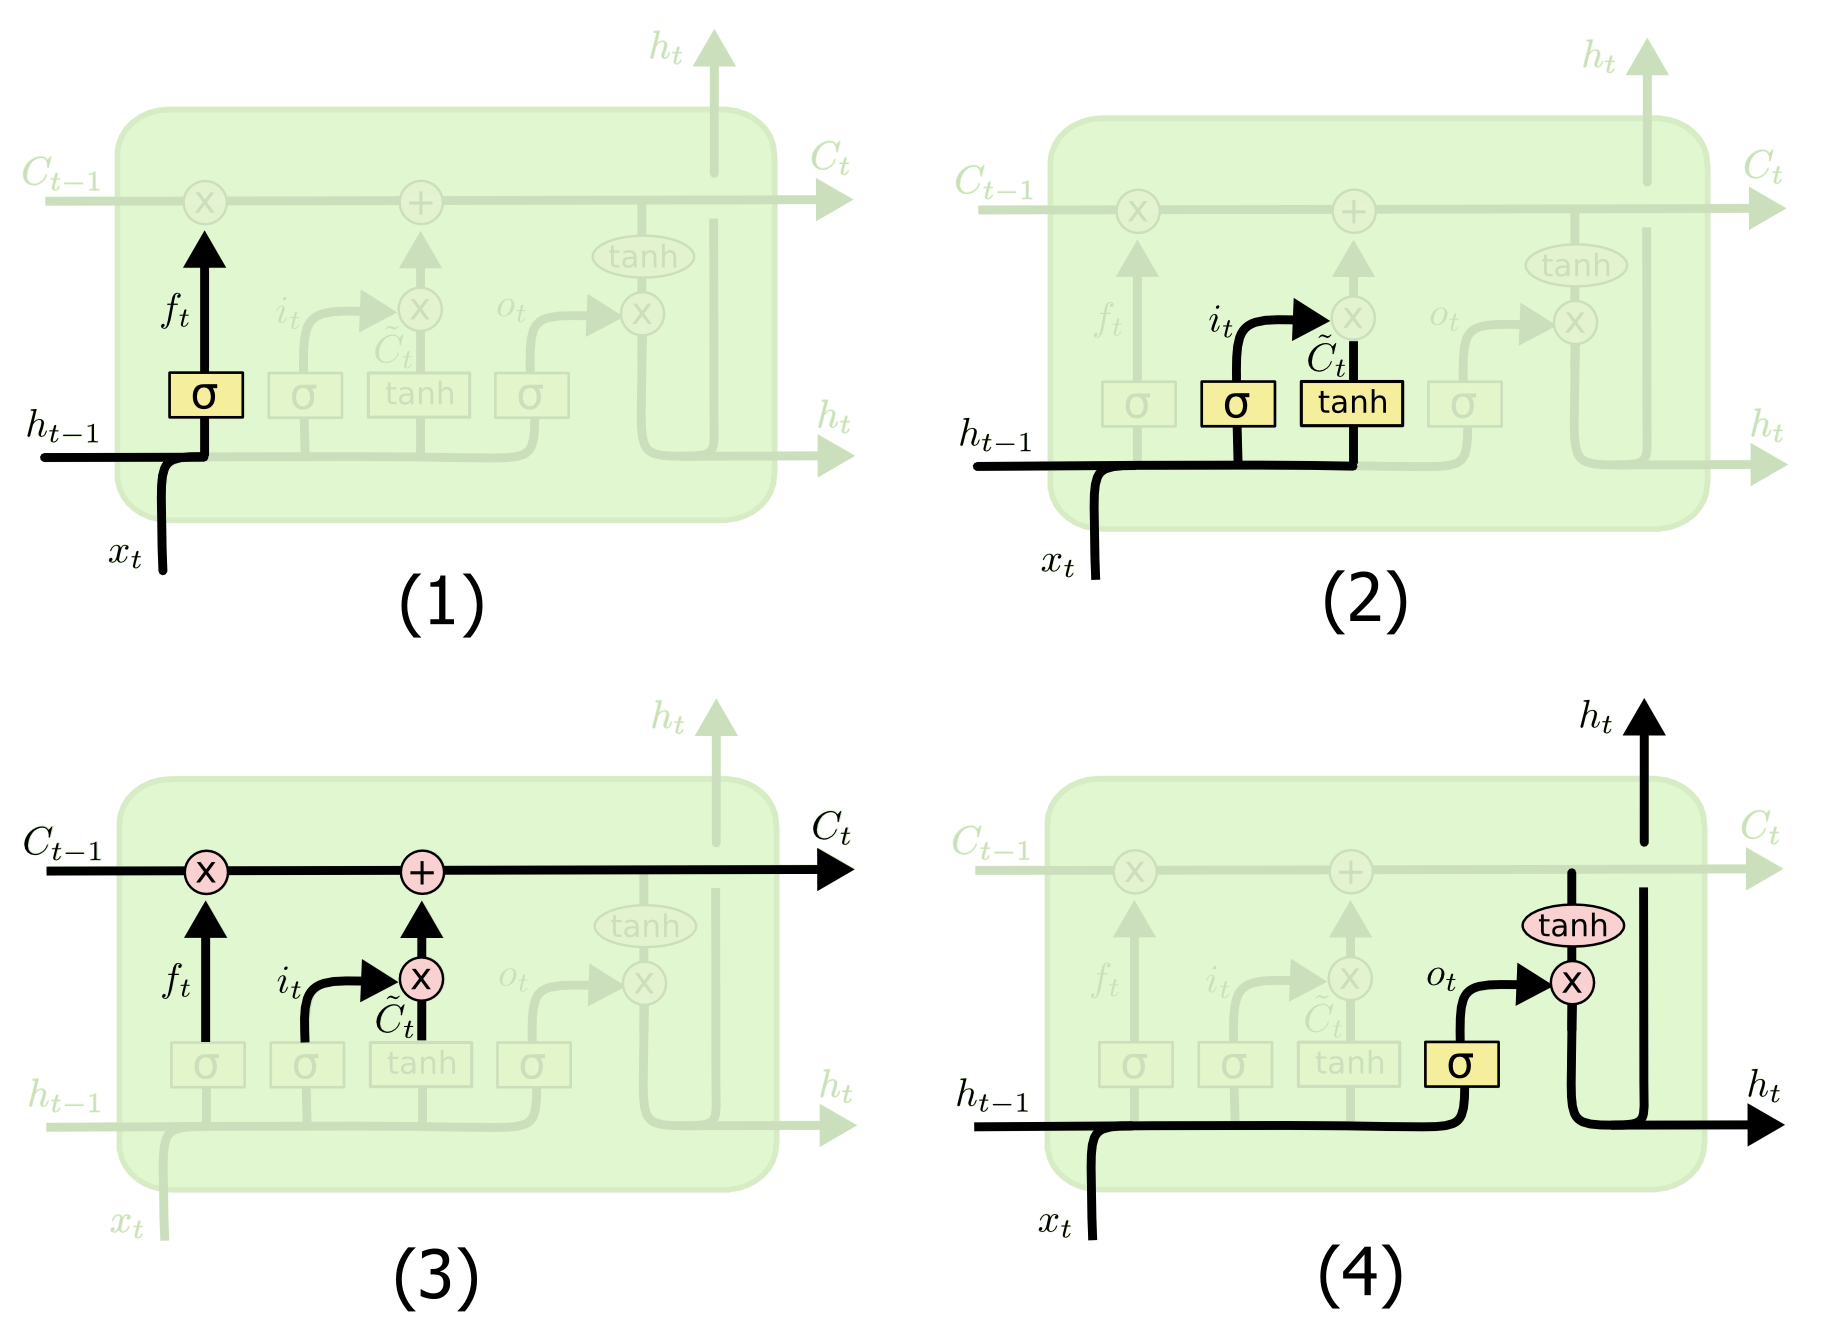
\includegraphics[height=3.5in]{Figures/LSTMs.png}
    \caption{ Recorrido por el funcionamiento de una celda LSTM. Figuras tomadas de \cite{olah}. }
    \label{LSTMrec}
  \end{center}
\end{figure}

En la figura \ref{LSTMrec}, se muestra el recorrido paso a paso del funcionamiento de una celda LSTM. 
El primer paso (panel 1) es decidir 
que parte de la información será descartada. Esta decisión se realiza por una sigmoide llamada en inglés ``\textit{forget gate layer}'':

\begin{equation}
  f_t = \sigma(W_f\cdot[h_{t-1},x_t]+b_f)
\end{equation}

Esta puerta recibe el input actual $x_t$ y la salida del tiempo anterior $h_{t-1}$ y arroja un valor entre 0 y 1, donde 0 significa
 `` olvidar esto completamente''  y 1 significa ``mantener esto completamente''. 

 El siguiente paso  (paneles 2 y 3)  se encarga de actualizar el estado de la celda del valor 
 de $C_{t-1}$ al nuevo valor $C_{t}$ y tiene dos partes, primero se multiplica el antiguo estado por $f_t$, y luego
 se suma el valor del nuevo candidato $C'_t$, escalado por un factor que cuantifica la magnitud del cambio:
 
 \begin{equation}
  C_t = f_t\cdot C_{t-1}+i_t\cdot C'_t
\end{equation}

donde,

 \begin{equation}
  i_t = \sigma(W_i\cdot[h_{t-1},x_t]+b_i)
\end{equation}

\begin{equation}
  C'_t = tanh(W_C\cdot[h_{t-1},x_t]+b_C)
\end{equation}



Finalmente, se calcula la salida $h_t$ de la siguiente manera (panel 4):

\begin{equation}
  o_t = \sigma(W_o\cdot[h_{t-1},x_t]+b_o)
\end{equation}

\begin{equation}
  h_t = o_{t}\cdot tanh(C_t)
\end{equation}

\section{Topología de los modelos utilizados}
Se han considerados 3 modelos que poseen una estructura básica que consta de una capa de entrada, dos o tres capas ocultas
y una capa de salida:


\begin{enumerate}
    \item \textbf{Modelo Denso}: En primer lugar se ha considerado un modelo que consta de dos capas densas, 
    en la figura \ref{Red_densa} podemos  ver  un resumen con las principales características de las mismas.
    \item \textbf{Modelo LSTM1}: En segundo lugar se ha considerado un modelo que contiene una capa LSTM y 
    una segunda capa densa (Fig. \ref{Red_LSTM1}).
    \item \textbf{Modelo LSTM2}: Por último se ha considerado un tercer modelo que consta de dos capas LSTM y una capa densa (Fig. \ref{Red_LSTM2}) que se 
    ha entrenado de manera secuencial.
    
    % utilizando únicamente los valores simulados de los caudales en la matriz $Y_{indv,id}$.
    % En este enfoque la red utiliza los valores de los caudales en tiempos anteriores
    %  $q_{t-1}, q_{t-2}, q_{t-n}$ para predecir el valor actual $q_{t}$. 
    %  La variable $n$ también llamada "look back" se puede elegir arbitrariamente y se puede ajustar haciendo 
    %  una busca con el método de cross validation.
\end{enumerate}

\begin{figure}[h!]
    \begin{center}
      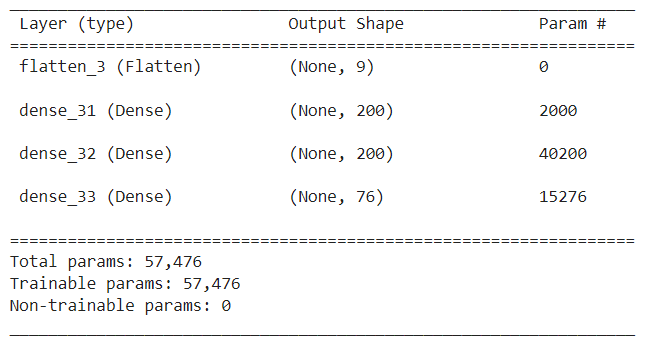
\includegraphics[height=2.in]{Figures/Red_densa.PNG}
      \caption{ Modelo Denso.}
      \label{Red_densa}
    \end{center}
  \end{figure}


  \begin{figure}[h!]
      \begin{center}
        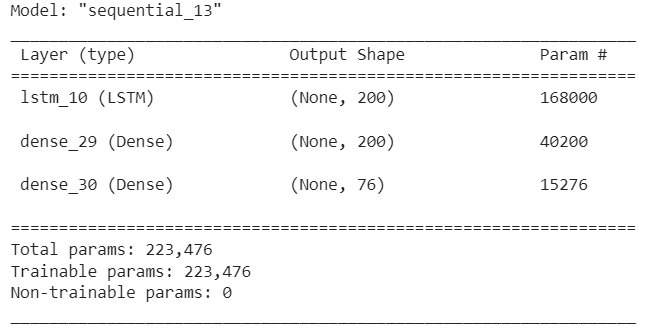
\includegraphics[height=2.in]{Figures/Red_LSTM.PNG}
        \caption{ Modelo LSTM1.}
        \label{Red_LSTM1}
      \end{center}
    \end{figure}
  
    \begin{figure}[h!]
        \begin{center}
          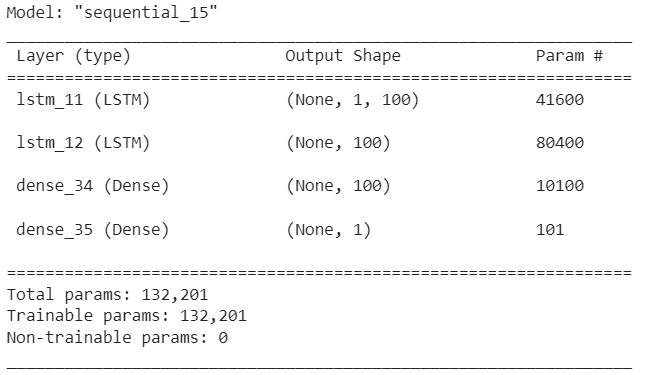
\includegraphics[height=2.1in]{Figures/Red_LSTM2.PNG}
          \caption{ Modelo LSTM2.}
          \label{Red_LSTM2}
        \end{center}
      \end{figure}
    
    

     
     

% \subsection{Modelo Denso}
% En primer lugar se ha considerado un modelo que consta de dos capas densas, en la figura \ref{Red_densa} podemos 
% ver  un resumen con las principales características de las mismas.
% \vspace{5mm}

% \begin{figure}[h!]
%     \begin{center}
%       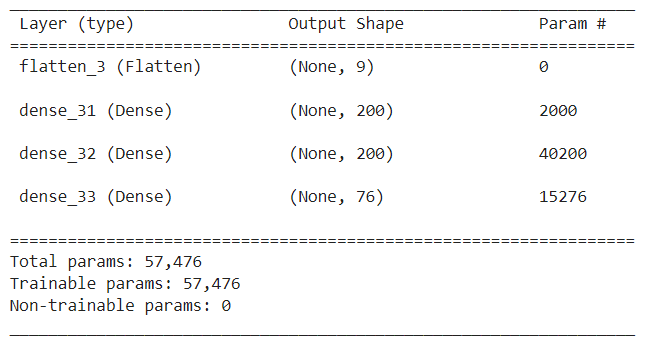
\includegraphics[height=2.in]{Figures/Red_densa.PNG}
%       \caption{ Modelo Denso}
%       \label{Red_densa}
%     \end{center}
%   \end{figure}


% \subsection{Modelo LSTM1}

% En segundo lugar se ha considerado un modelo que contiene una capa compuesta de una red recurrente y una segunda capa densa (Fig. \ref{Red_LSTM1})
% Se han utilizado dos maneras diferentes de entrenar este modelo, por un lado se ha entrenado sobre toda la cuenca,
% de la misma manera que el modelo denso, es decir utilizando las matrices $X_{comp}$ e $Y_{comp}$, 
% \begin{figure}[h!]
%     \begin{center}
%       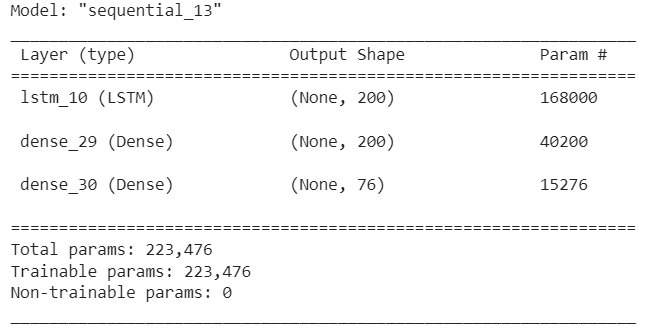
\includegraphics[height=2.in]{Figures/Red_LSTM.PNG}
%       \caption{ Modelo LSTM 1 }
%       \label{Red_LSTM1}
%     \end{center}
%   \end{figure}

%   \vspace{5mm}

% \subsection{Modelo LSTM2}

% \begin{figure}[h!]
%     \begin{center}
%       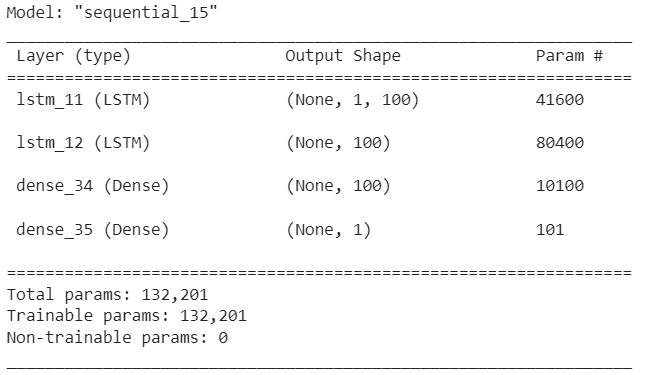
\includegraphics[height=2.in]{Figures/Red_LSTM2.PNG}
%       \caption{ Modelo LSTM 2}
%       \label{Red_LSTM2}
%     \end{center}
%   \end{figure}


% Por último se ha considerado un tercer modelo que consta de dos capas LSTM y una capa densa (Fig. \ref{Red_LSTM2}).




\subsection{Regularización de la función de coste}
Se han considerado dos tipos de regularizaciones, L1 y L2 que penalizan el loss añadiendo
los siguientes términos para cada caso:

\begin{equation}
    loss + \lambda \sum |\omega_ij| ~~(L1)
\end{equation}

\begin{equation}
    loss + \lambda \sum \omega^2_ij ~~(L2)
\end{equation}

La función de estos términos extra es la de reducir el valor de los parámetros haciendo incluso que la influencia de 
algunas variables de entrada sea nula en la salida de la red, lo que da lugar a una selección de variables de forma natural y
reduce el posible sobreajuste de los datos. El valor de $\lambda$ varía entre 0 y 1 y controla la magnitud
de la reducción de los parámetros. 


\subsection{Funciones de activación}
En todas las capas se ha considerado la misma función de activación $f$, y se han entrenado los modelos considerando 
las opciones mostradas en \ref{activation}.

\begin{table}[h!]
    \centering
    \begin{tabular}{|c|c|}   
        \hline
        &\\
     $ f(x)= \frac{1}{e^{-x}+1}$ ~(sigmoide) & 
     $f(x) = \left\lbrace
     \begin{array}{ll}
     0 &\textup{si } x\leq 0 \\
     x & \textup{si } x > 0 
     \end{array}
     \right. ~(relu)$    \\
     &\\
     \hline
     &\\
     $f(x)= \frac{e^{2x}-1}{e^{2x}+1} ~(tanh)$ & $f(x)=x ~ (linear)$    \\ 
     &\\
     \hline
    \end{tabular}
    \caption{ Funciones de activación}
    \label{activation}
    \end{table}


\subsection{Optimizadores}

\begin{figure}[h!]
  \begin{center}
    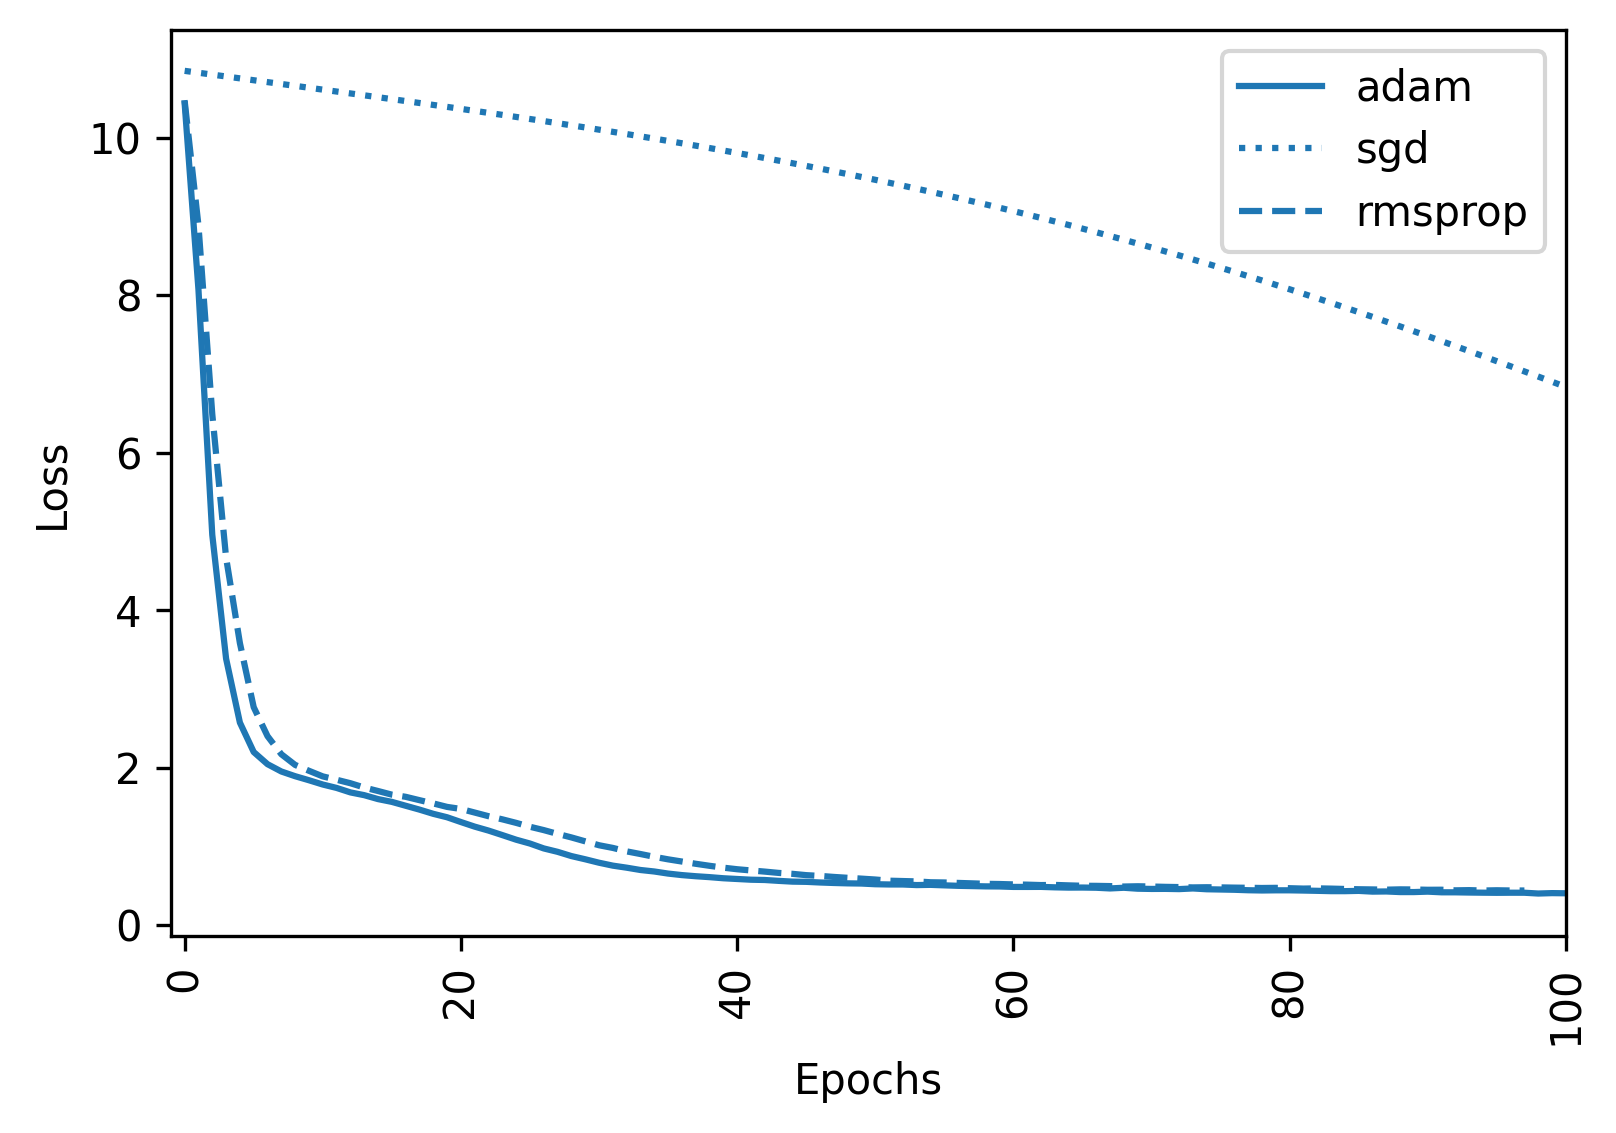
\includegraphics[height=3.in]{Figures/optims.png}
    \caption{ Evolución de la función de loss considerando diferentes optimizadores.}
    \label{opt}
  \end{center}
\end{figure}

Dado el gran número de diferentes pesos y observaciones, el cálculo de la derivada parcial de la función de coste 
respecto a cada uno de los pesos de la red para cada observación es inviable. Existen diferentes métodos que optimización
este proceso y agilizan los cálculos. En este trabajo se ha hecho una exploración inicial manual para evaluar 
la performance de los optimizadores 
"\textit{Stochastic Gradient Descent}" (SGD) \cite{optim}, "\textit{Adaptive moment estimation}" (Adam) \cite{adam} y 
\textit{Root Mean Square Propagation} (RMSprop) \cite{optim}.



En la figura \ref{opt} se muestra a modo de ejemplo la evolución de la función de loss considerando cada uno de los 
optimizadores al entrenar el modelo LSTM1, se puede ver que la taza de aprendizaje con adam y rmspror es considerablemente
mayor que con sgd, ya que en los primeros casos la función de loss alcanza su valor de equilibrio en aproximadamente 
60 épocas, mientras que sgd necesita más de 200. 



\subsection{Calibración de los modelos}
\label{cal}

\begin{figure}[h!]
  \begin{center}
    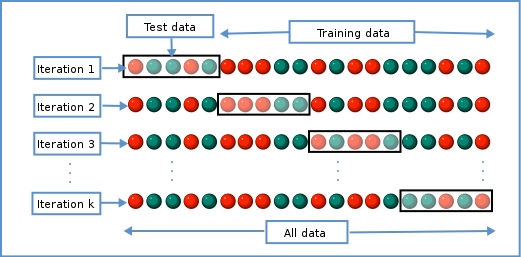
\includegraphics[height=2.in]{Figures/GridsearchCV.png}
    \caption{ k-fold cross validation (imagen de Gufosowa - WikiMedia).}
    \label{KCV}
  \end{center}
\end{figure}


Los modelos se calibran realizando una búsqueda exhaustiva de hyper-parámetros utilizando el 
con el método "GridSearchCV" disponible en la librería scikit-learn \cite{scikit}.
Éste método crea una grilla con los hyper-parámetros del modelo y optimiza sus valores realizando una búsqueda
 con validación cruzada, en donde el conjunto de datos se divide en datos de entrenamiento y de validación 
 (train/test en la figura \ref{KCV}).  Cómo este conjunto se divide y cuantas veces se realiza el proceso, se controla mediante el 
 número de pliegues o folds, en general denotado con la letra k.
 El modelo utiliza el primer fold en la primera iteración como conjunto de test y 
 los siguientes k-1 como conjunto de train. Este proceso se repite k veces para cada uno de las posibles 
 combinaciones de hyper-parámetros presentes en la grilla y arroja como resultado final un valor promedio 
 del escore utilizado para evaluar  la calidad del modelo. 

 \begin{table}[h!]
  \begin{center} 
  \begin{tabular}{|l|l|l|}
    \hline
   Modelo&Parámetros &  valores \\
   \hline
   &solver &  rmsprop, adam, sgd\\
   &Neuronas &  10, 80, 200 \\
   Denso &activación & sigmoid,relu,tanh,linear \\
   &alpha &  0.0001,0.0002,0.0003 \\
   &Regularización & l1,l2 $\lambda = 0.0001,0.001,0.1$  \\
   \hline
   &solver &   rmsprop, adam, sgd\\
   &Neuronas &  10, 80, 200 \\
   LSTM1 PCA &activación & sigmoid,relu,tanh,linear \\
   &alpha &  0.0001,0.0002,0.0003 \\
   &Regularización & l1,l2 $\lambda =0.0001,0.001,0.1$  \\

   \hline
   &solver &   rmsprop, adam, sgd\\
   &Neuronas &  10, 80, 200 \\
   LSTM1 loc &activación & sigmoid,relu,tanh,linear \\
   &alpha &  0.0001,0.0002,0.0003 \\
   &Regularización & l1,l2 $\lambda =0.0001$  \\

   \hline
   &solver &   rmsprop, adam, sgd\\
   &Neuronas &  10, 80, 200 \\
   LSTM2 &activación & sigmoid,relu,tanh,linear \\
   &alpha & 0.001 \\
   &Regularización & l1,l2 $\lambda =0.0000001$  \\
   \hline

  \end{tabular}
  \caption{ Hyper parámetros explorados en los diferentes modelos.}
  \label{hyper}
\end{center}
  \end{table}


  En la tabla \ref{hyper} se muestran los hyper-parámetros explorados para entrenar los diferentes modelos. En el caso
  del entrenamiento global, realizado para los modelos denso y LSTM1 PCA, tres de 
  estos parámetros (el número de neuronas, la función de activación y $\lambda$) 
  han sido optimizados mediante el método GridSearchCV.


  \section{Entrenamiento}
  Los modelos han sido entrenados durante un número de épocas o pasos
  igual a 200 y se ha utilizado el callback "\textit{early stopping}" con paciencia 3, 
  que interrumpe la ejecución cuando el valor del loss en el conjunto de validación aumenta durante tres iteraciones sucesivas. 
Se han considerado tres métodos diferentes de entrenamiento que se describen a continuación.

% \begin{itemize}
%     \item Entrenamiento global, considerando las series hidro-climáticas de entrada de la cuenca en su totalidad 
%     \item Entrenamiento local,  considerando las series hidro-climáticas de entrada locales para cada sub-cuenca.
%     \item Secuencial, considerando los datos de las series temporales de salida de manera secuencial.
% \end{itemize}en primer lugar se han entrenado los 
 
  \subsection{Entrenamiento global}
 Los modelos denso y LSTM1 han sido entrenados sobre una matriz que contiene las entradas o variables características 
 (series temporales de precipitación, temperatura máxima y temperatura mínima) para 
todas las subcuencas que constituyen la cuenca hidrológica Chambo:
  
  \vspace{5mm}
  
    \begin{equation*}
      X_{comp}= 
      \begin{bmatrix}
          p_{1,1} & T^{max}_{1,1} &  T^{min}_{1,1}& p_{1,2} & T^{max}_{1,2} &  T^{min}_{1,2} & ... &p_{1,nc} & T^{max}_{1,nc} &  T^{min}_{1,nc} \\
          ... & ... &  ...& ... & ...&  ... & ... &... & ... &  ... \\
          p_{nt,1} & T^{max}_{nt,1} &  T^{min}_{nt,1}& p_{nt,2} & T^{max}_{nt,2} &  T^{min}_{nt,2} & ... &p_{nt,n} & T^{max}_{nt,n} &  T^{min}_{nt,nc} \\
          \end{bmatrix}
  \end{equation*}
  
  \vspace{5mm}
  
  
  Donde $n_t$ es el número de pasos temporales y $nc$ es el número de subcuencas. 
  Las variables objetivo son los caudales naturales simulados con el modelo hidrológico LEM y 
  se encuentran almacenados en una matriz $Y_{comp}$ estructurada de la siguiente manera:
  
  \vspace{5mm}
  
  \begin{equation*}
      Y_{comp}= 
      \begin{bmatrix}
          q_{1,1} & q_{1,2} & q_{1,2} ... &  q_{1,nc} \\
          ... & ... & ... &  ... \\
          q_{nt,1} & q_{nt,2} & q_{nt,2} ... &  q_{nt,nc} \\
          \end{bmatrix}
  \end{equation*}
  
  \vspace{5mm}
  
  El paso  de tiempo que se ha considerado es mensual y el rango temporal total es de 20 años 
  (desde el año 2000 hasta el año 2020). Por otro lado la cuenca se encuentra compuesta por 76 subcuencas, 
  entonces las dimensiones de $X_{comp}$ e $Y_{comp}$ son (229,228) y (229,76), respectivamente.
  Finalmente, los datos han sido divididos en conjuntos de train y test tomando los primeros 160 
  como conjunto de train y los últimos 69 como conjunto de test.

  Para el caso de capas LSTM es necesario agregar una dimensión a las matrices de entrada que toma en cuenta la correlación temporal de las muestras. 
  La estructura de las matrices de entrada toman la forma (\textit{muestras}, \textit{pasos de tiempo}, \textit{características}). En el modelo 
  LSTM1 se considera un paso de tiempo por cada muestra, por lo cual  las matrices toman 
  la dimensión (229,1,228) y (229,1,76), respectivamente.

\subsection{Entrenamiento local}
 Por otro lado el modelo LSTM1 también se ha entrenado individualmente cuenca por cuenca, para lo cual se han utilizado
matrices $X_{loc}$ e $Y_{loc}$ con las siguientes formas:
\vspace{5mm}

\begin{equation*}
    X_{loc,id}= 
    \begin{bmatrix}
        p_{1,id} & T^{max}_{1,id} &  T^{min}_{1,id} \\
        ... & ... &  ... \\
        p_{nt,id} & T^{max}_{nt,id} &  T^{min}_{nt,id} \\
        \end{bmatrix}
\end{equation*}

\vspace{5mm}


\begin{equation*}
    Y_{loc,id}= 
    \begin{bmatrix}
        q_{1,id}  \\
        ...  \\
        q_{nt,id}  \\
        \end{bmatrix}
\end{equation*}

\vspace{5mm}

Donde $id$ es el número de la subcuenca. 
\vspace{5mm}

En este último caso, las matrices poseen las dimensiones (229,1,3) y (229,1,1), respectivamente. 
La división entre los conjuntos de entrenamiento y test se ha hecho de la misma manera que en el apartado anterior.

\subsection{Entrenamiento secuencial}

Finalmente, el modelo LSTM2 se ha entrenado de manera secuencial, utilizando únicamente los valores simulados de los caudales 
en la matriz $Y_{loc,id}$. En este enfoque, la red utiliza los valores de los caudales en tiempos anteriores
 $q_{t-1}, q_{t-2}, q_{t-n}$ para predecir el valor actual $q_{t}$. 
 La variable $n$ también llamada "look back" se puede elegir arbitrariamente y se puede ajustar haciendo 
 una busca con el método de cross-validation.


\section{Análisis de componentes principales}

El espacio de variables predictoras del conjunto de entrenamiento 
que contiene la información de las 76 subcuencas posee una dimensión: (160,228).
Sin embargo, existen correlaciones entre las variables que 
provocan que muchas de estas aporten información poco relevante o redundante \cite{Manu}. 
Estas correlaciones pueden distorsionar el proceso de aprendizaje de los modelos \cite{gutierrez} 
y es por eso que se ha optado por reducir el número de variables mediante el análisis de componentes principales\cite{PCA}.

Este método realiza una transformación del espacio predictor a un espacio vectorial 
cuya base son los auto-vectores de la matriz de covariancia. 
En este espacio, los valores en la diagonal de dicha matriz son las varianzas
en la dirección de cada uno de los vectores de la base o componentes principales.
La reducción de dimensiones se realiza escogiendo las direcciones que captan la mayor variación 
de los datos originales, es decir las PCA con las mayores varianzas. 

Luego de realizar este análisis se ha encontrado que se puede explicar el 96$\%$ de la varianza del conjunto
de datos original considerando sólo las primeras 9 componentes (ver figura \ref{PCA}). Por lo tanto la reducción del espacio
predictor es considerable, ya que ha pasado de ser (160,228) a (160,9).

\begin{figure}[h!]
  \begin{center}
    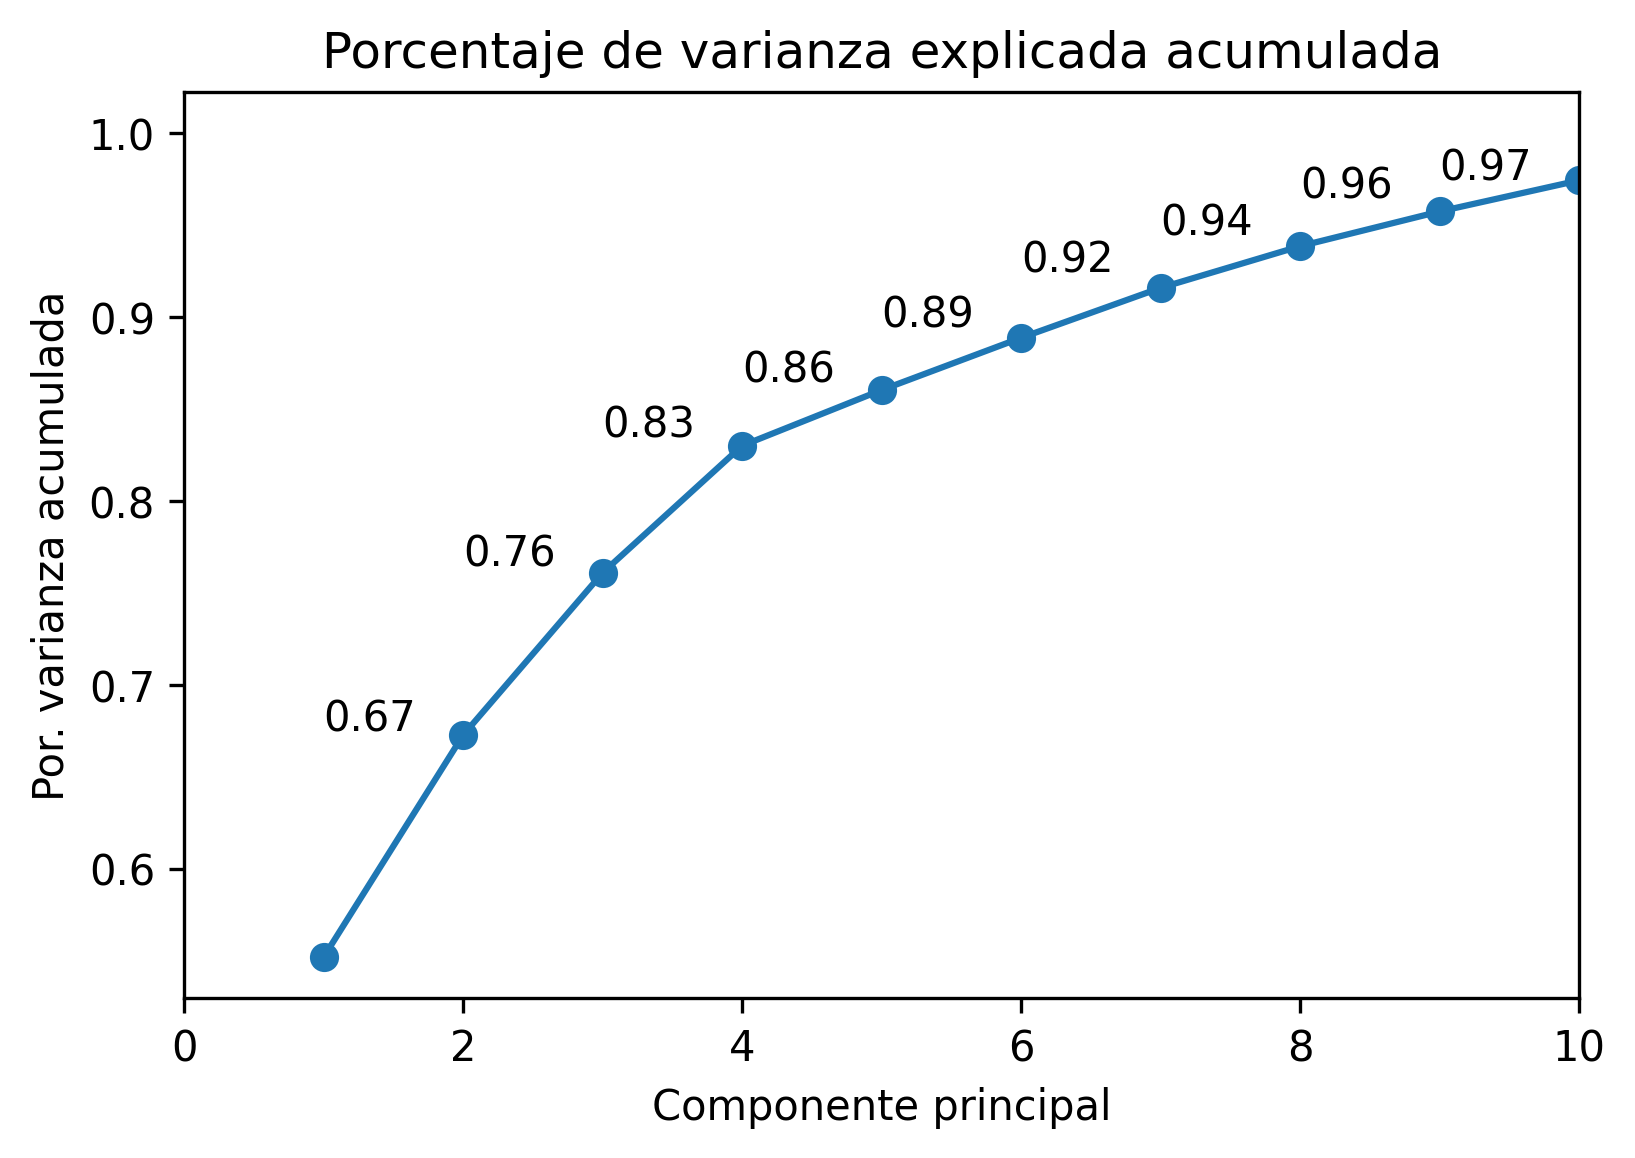
\includegraphics[height=2.5in]{Figures/PCA.png}
    \caption{ Porcentaje de varianza explicada acumulada para las primeras 9 componentes principales.}
    \label{KCV}
  \end{center}
\end{figure}

\section{Coeficiente de Nash-Sutcliffe}
\label{sectNSE}


\begin{table}[h!]
  \begin{center}
  \begin{tabular}{|c|c|}
    \hline
    Calidad del ajuste &   NSE  \\
    \hline
     &   \\
   Excelente & $0.75 < NSE \leq 1.00$   \\
   Bueno &  $0.65<  NSE \leq 0.75$ \\
   Aceptable &  $0.5<  NSE \leq 0.65$  \\
   No aceptable &  $ NSE \leq 0.5$ \\
   &   \\
   \hline
  \end{tabular}
  \caption{Calidad de los ajustes en función del coeficiente NSE \cite{NSE}.}
  \label{tablaNSE}
\end{center}
  \end{table}

Además de utilizar la función de loss para validar los modelos durante el entrenamiento, 
también se ha utilizado el coeficiente Nash-Sutcliffe (NSE) \cite{NSE} para evaluar la performance de los mismos en el conjunto de test. 
Este coeficiente es uno de los más utilizados en hidrología y se define de la siguiente manera:

\begin{equation}
  NSE = 1-\frac{\sum^n_i(y_i-\hat{y}_i)^2}{\sum^n_i(\bar{y}-\hat{y}_i)^2}
\end{equation}

Los valores de NSE varían entre $-\infty$ y 1, siendo este último valor el correspondiente a un ajuste perfecto.
En la tabla \ref{tablaNSE} se indica la relación entre los valores de NSE y la calidad de los ajustes.
Este coeficiente equivale a una combinación lineal del error medio
cuadrático, la desviación y el coeficiente de correlación
entre las series.


%  \subsection{Validación de los modelos}

%  \begin{figure}[h!]
%    \begin{center}
%      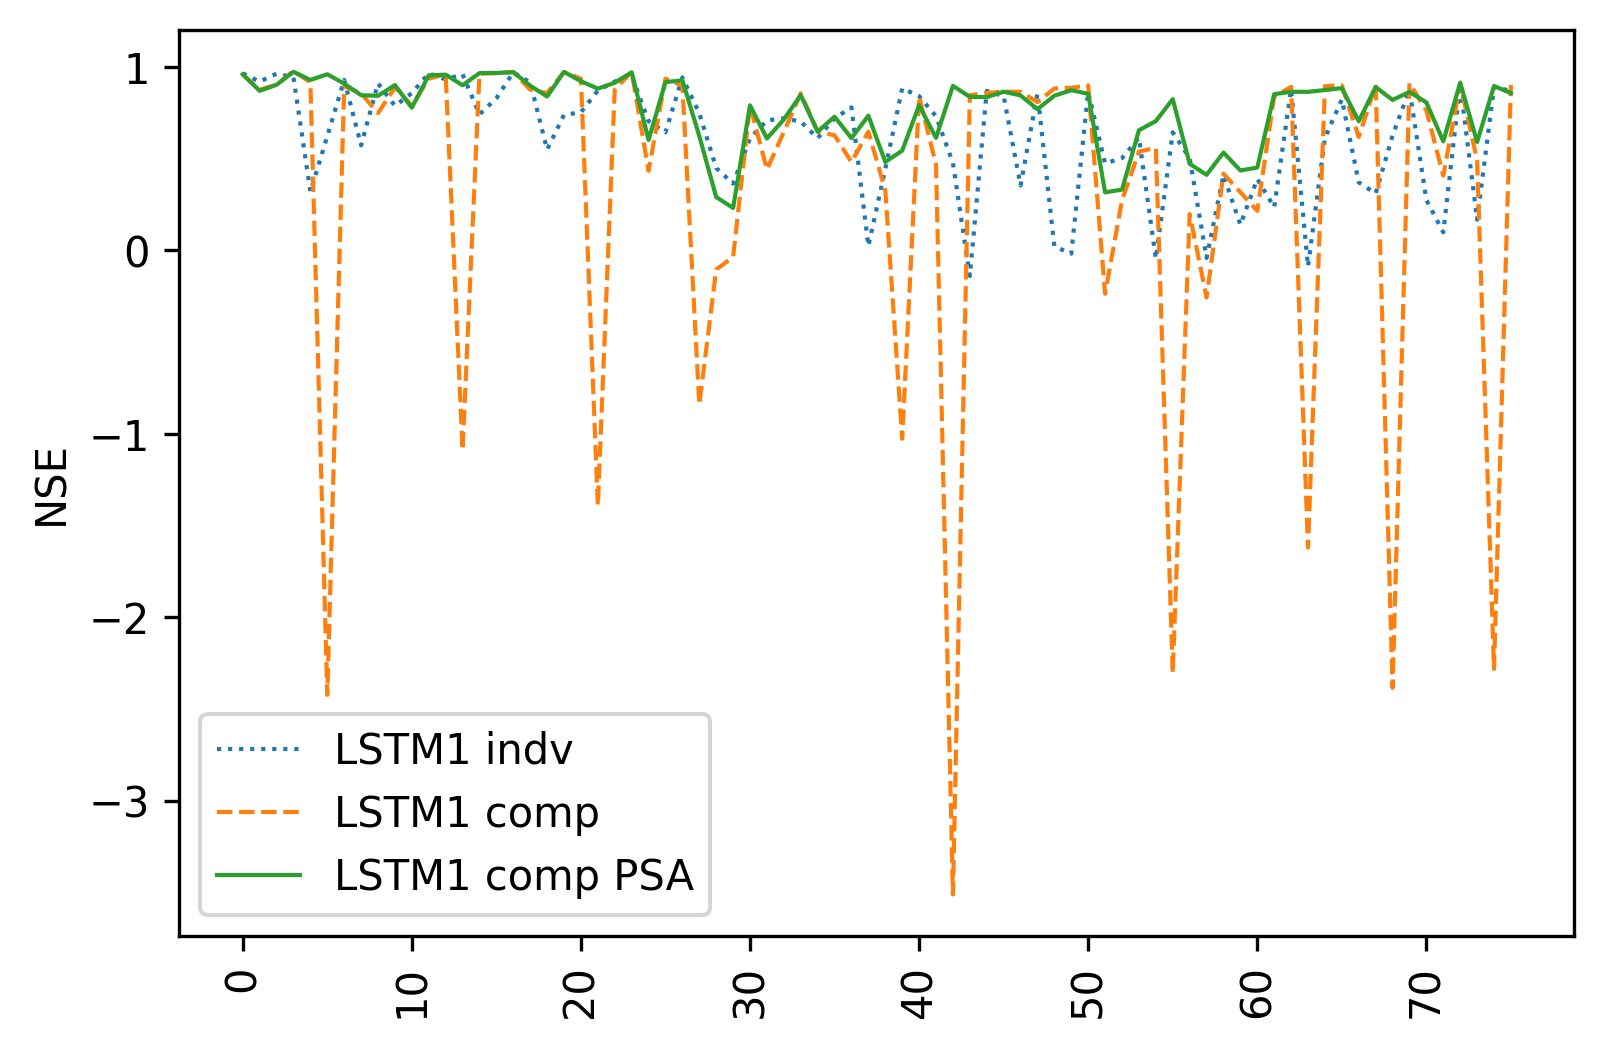
\includegraphics[height=3.in]{Figures/NSEs_1.png}
%      \caption{ Modelo LSTM 2}
%      \label{NSE1}
%    \end{center}
%  \end{figure}

% Para validar los modelos y hacer un análisis un poco más profundo de cómo es su performance en los diferentes puntos
% de la cuenca, se ha utilizado el coeficiente de Nash-Sutcliffe (NSE). En la figura \ref{NSE1} se muestran los valores obtenidos 
% de NSE en todas las subcuencas para el modelos LSTM1. La curva punteada muestra los valores obtenidos al entrenar el modelo en 
% cada subcuenca de forma individual, la curva dashed es la obtenida entrenando el modelo para toda la cuenca en conjunto
% considerando la matriz$X_{comp}$ que posee 288 características. Se puede observar que para este modelo, 
% el valor de NSE baja considerablemente en muchos puntos, esto se debe a que al haber tantas características 
% de entrada se produce un sobre ajuste de los datos. Esto se puede corregir haciendo una reducción del espacio considerando
% las componente principales (curva sólida). En este análisis el número de características se reduce a 9 componentes principales 
% que explican el $96\%$ de la varianza de los datos.

% %   \begin{figure}[h!]
% %     \begin{center}
% %       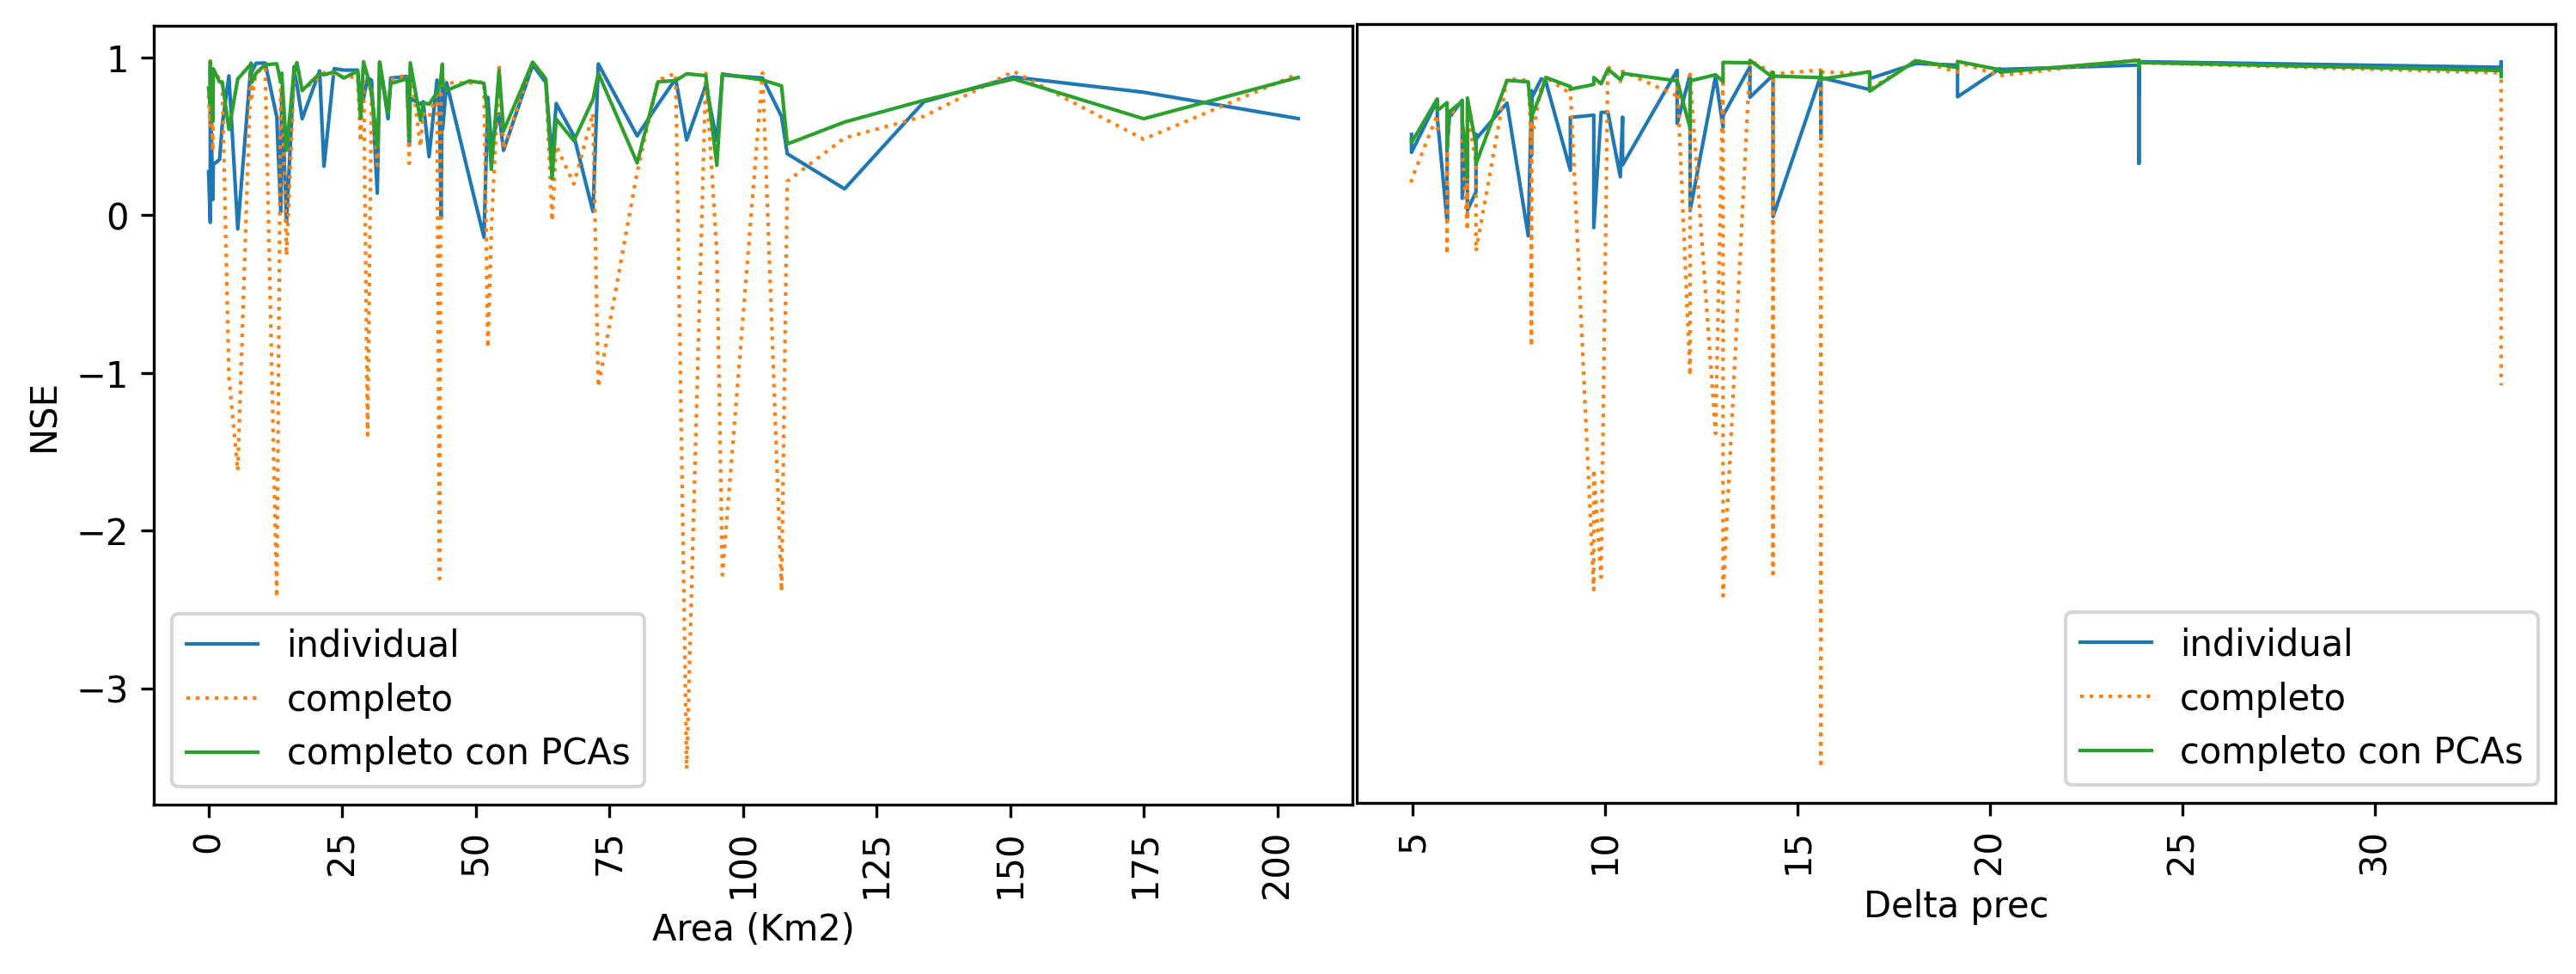
\includegraphics[height=2.3in]{Figures/NSEs_Area_prec.png}
% %       \caption{ Modelo LSTM 2}
% %       \label{NSEs_Area_prec}
% %     \end{center}
% %   \end{figure}

%    \begin{figure}
%    \centering
%    \begin{subfigure}[b]{1\textwidth}
%        \centering
%        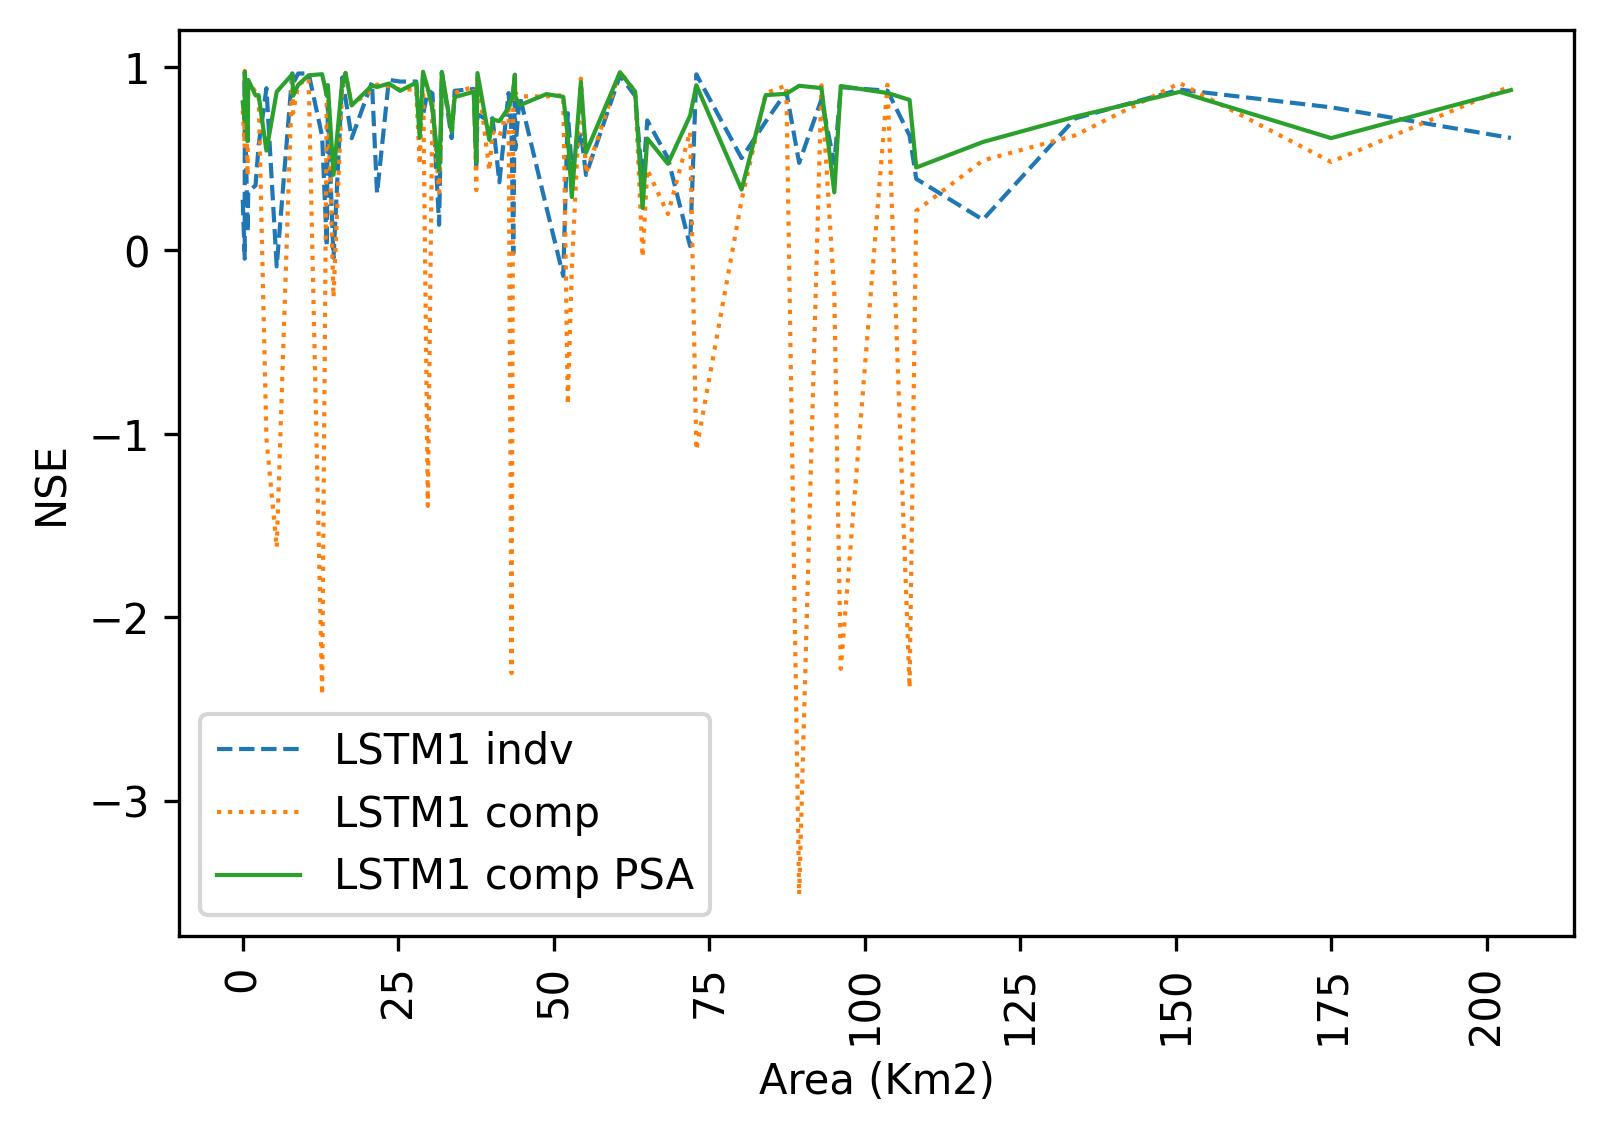
\includegraphics[width=\textwidth]{Figures/NSEs_Area.png}
%        \caption{}
%        \label{area}
%    \end{subfigure}
%    \hfill
%    \begin{subfigure}[b]{1\textwidth}
%        \centering
%        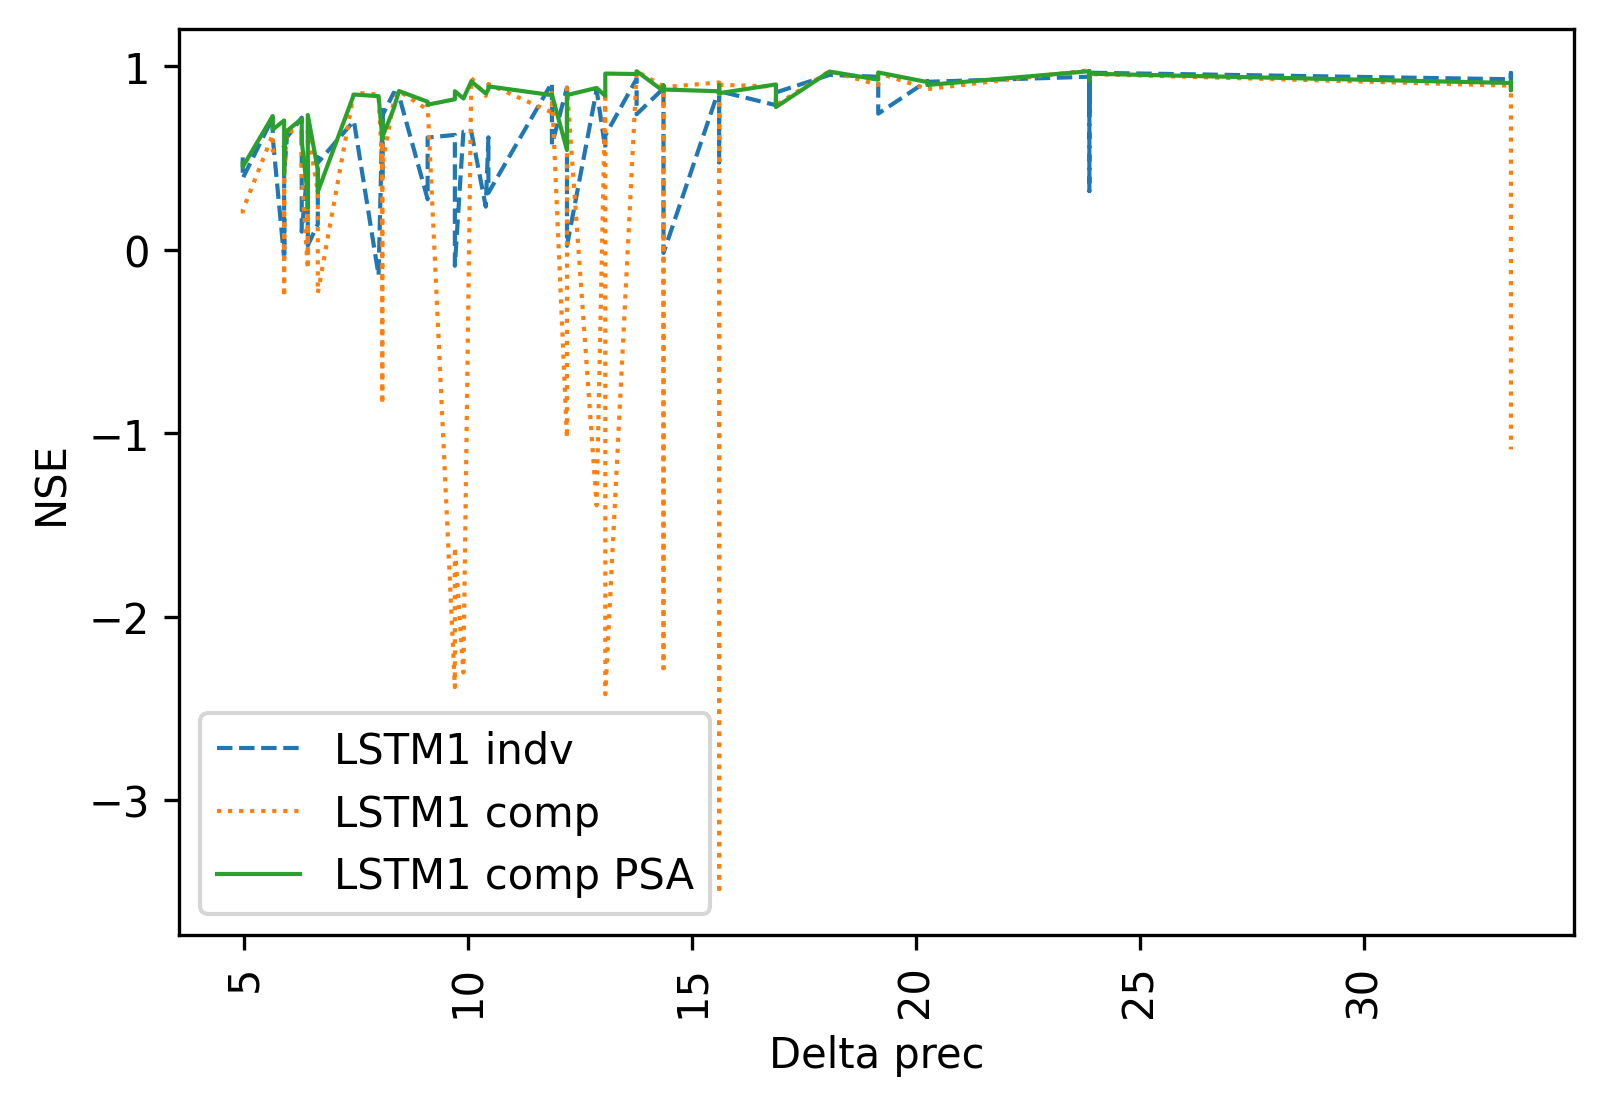
\includegraphics[width=\textwidth]{Figures/NSEs_Delta prec.png}
%        \caption{}
%        \label{Dp}
%    \end{subfigure}
%       \caption{Coeficientes de Nash-Sutcliffe en función del área (\ref{area}) y la variación de presión (\ref{Dp}).}
%       \label{NSEs_Area_prec}
% \end{figure}



%  Con el fin de determinar si hay otros factores que provocan el sobre ajuste de los datos,
%  en la figura \ref{NSEs_Area_prec} se muestran los valores de NSE en función del área de las cuencas (panel izquierdo) y 
%  de   la variación máxima de precipitación (panel derecho). Se puede observar que los modelos tienden a fallar 
%  para cuencas con áreas pequeñas ($A<125~km^2$) y cuando la serie de precipitación no muestra grandes variaciones 
%  ($\Delta P < 20~mm/d$). Esto se debe a que en este caso es difícil para los modelos poder distinguir los verdaderos patrones 
%  de precipitación del ruido, una alternativa para mejorar estos resultados sería considerar una capa de autoencoder al 
%  inicio de los modelos que permitan filtrar el ruido en los datos. 
 
%  Este efecto es aún más visible cuando entrenamos los modelos 
%  de manera local, si comparamos la curva continua con la dashed, podemos ver que en la mayoría de los casos, los resultados obtenidos
%  entrenando el modelo en toda la cuenca son mejores que cuando lo hacemos de manera individual. Esto se debe a que en el primer caso
%  estamos considerando  los patrones de precipitación en diferentes puntos de la cuenca, y aunque localmente 
%  la variación de la precipitación sea pequeña, la red aprende a completar la información faltante utilizando 
%  la información de toda la cuenca. En el segundo caso sólo  consideramos   los patrones locales en una cuenca dada y si la información
%  otorgada por la serie de precipitación no es buena (la variación es pequeña y no se reconoce un patrón claro) la red  
% no es capaz de completar la información necesaria con información proveniente de otros puntos de la cuenca. 

% * Agregar coeficiente NSE 
% * Agregar descripcion sobre la grilla de parametros con tabla y alguna graficas
% * Agregar lo de las PCAs

% \section{Resultados}
% * Agregar funciones de loss
% * Graficas de las distribuciones de los pesos? para ver que patrones se forman?

% \begin{figure}[h!]
%     \begin{center}
%       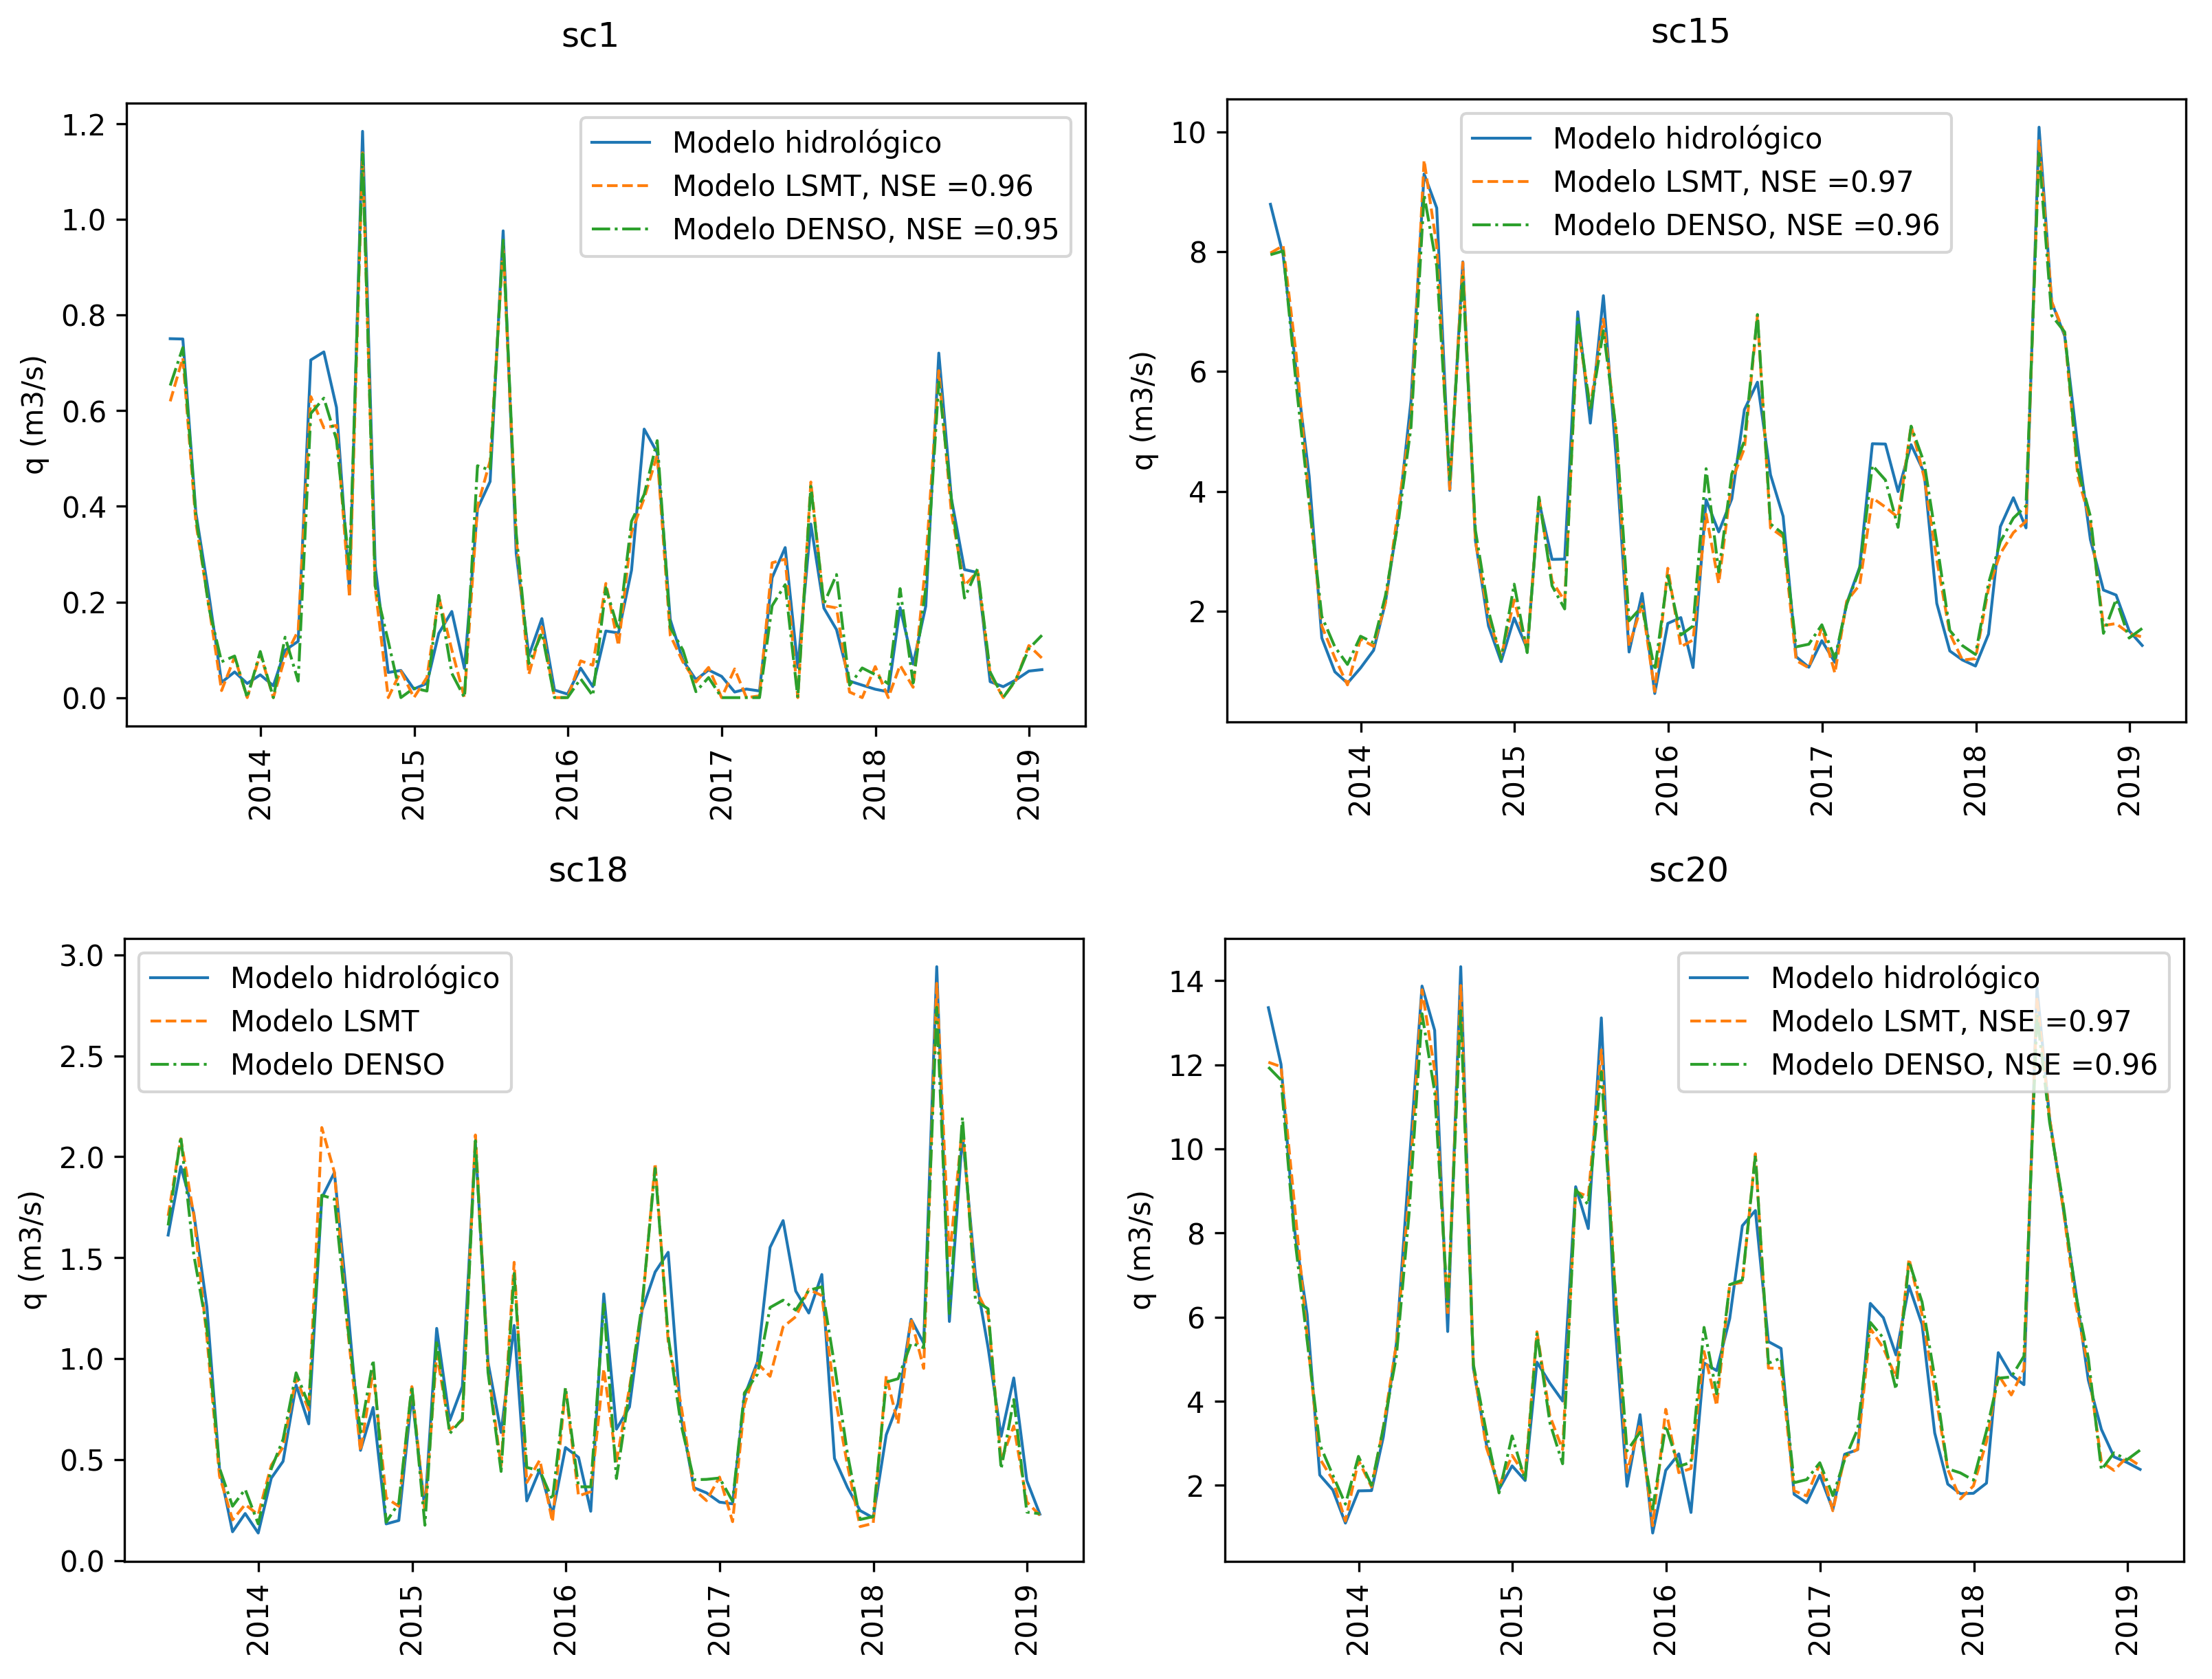
\includegraphics[height=4.in]{Figures/comparacion_scs.png}
%       \caption{ Resultados del Modelo LSTM 2.}
%       \label{autocorrelacion}
%     \end{center}
%   \end{figure}

% En la figura \ref{resultados_q} se muestran a modo de ejemplo los resultados obtenidos para los caudales de tres puntos
% diferentes de la cuenca, la sub-cuenca 1 , la sub-cuenca 20 y la 73 .
% En las figuras se muestran los resultados de los caudales simulados con el modelo hidrológico y los obtenidos con 
% los modelos Denso y LSTM1 en el conjunto de test. Se puede apreciar que agregar una capa LSTM mejora ligeramente los resultados
% ya que se incrementa el valor del coeficiente Nash-Sutcliffe (NSE) para el modelo. Esto era de esperar ya que la red LSTM
% tiene en consideración la dependencia temporal de las diferentes entradas mientras que el modelo denso considera las entradas
% de los distintos pasos de tiempo como independientes. 



% \begin{figure}[h!]
%     \begin{center}
%       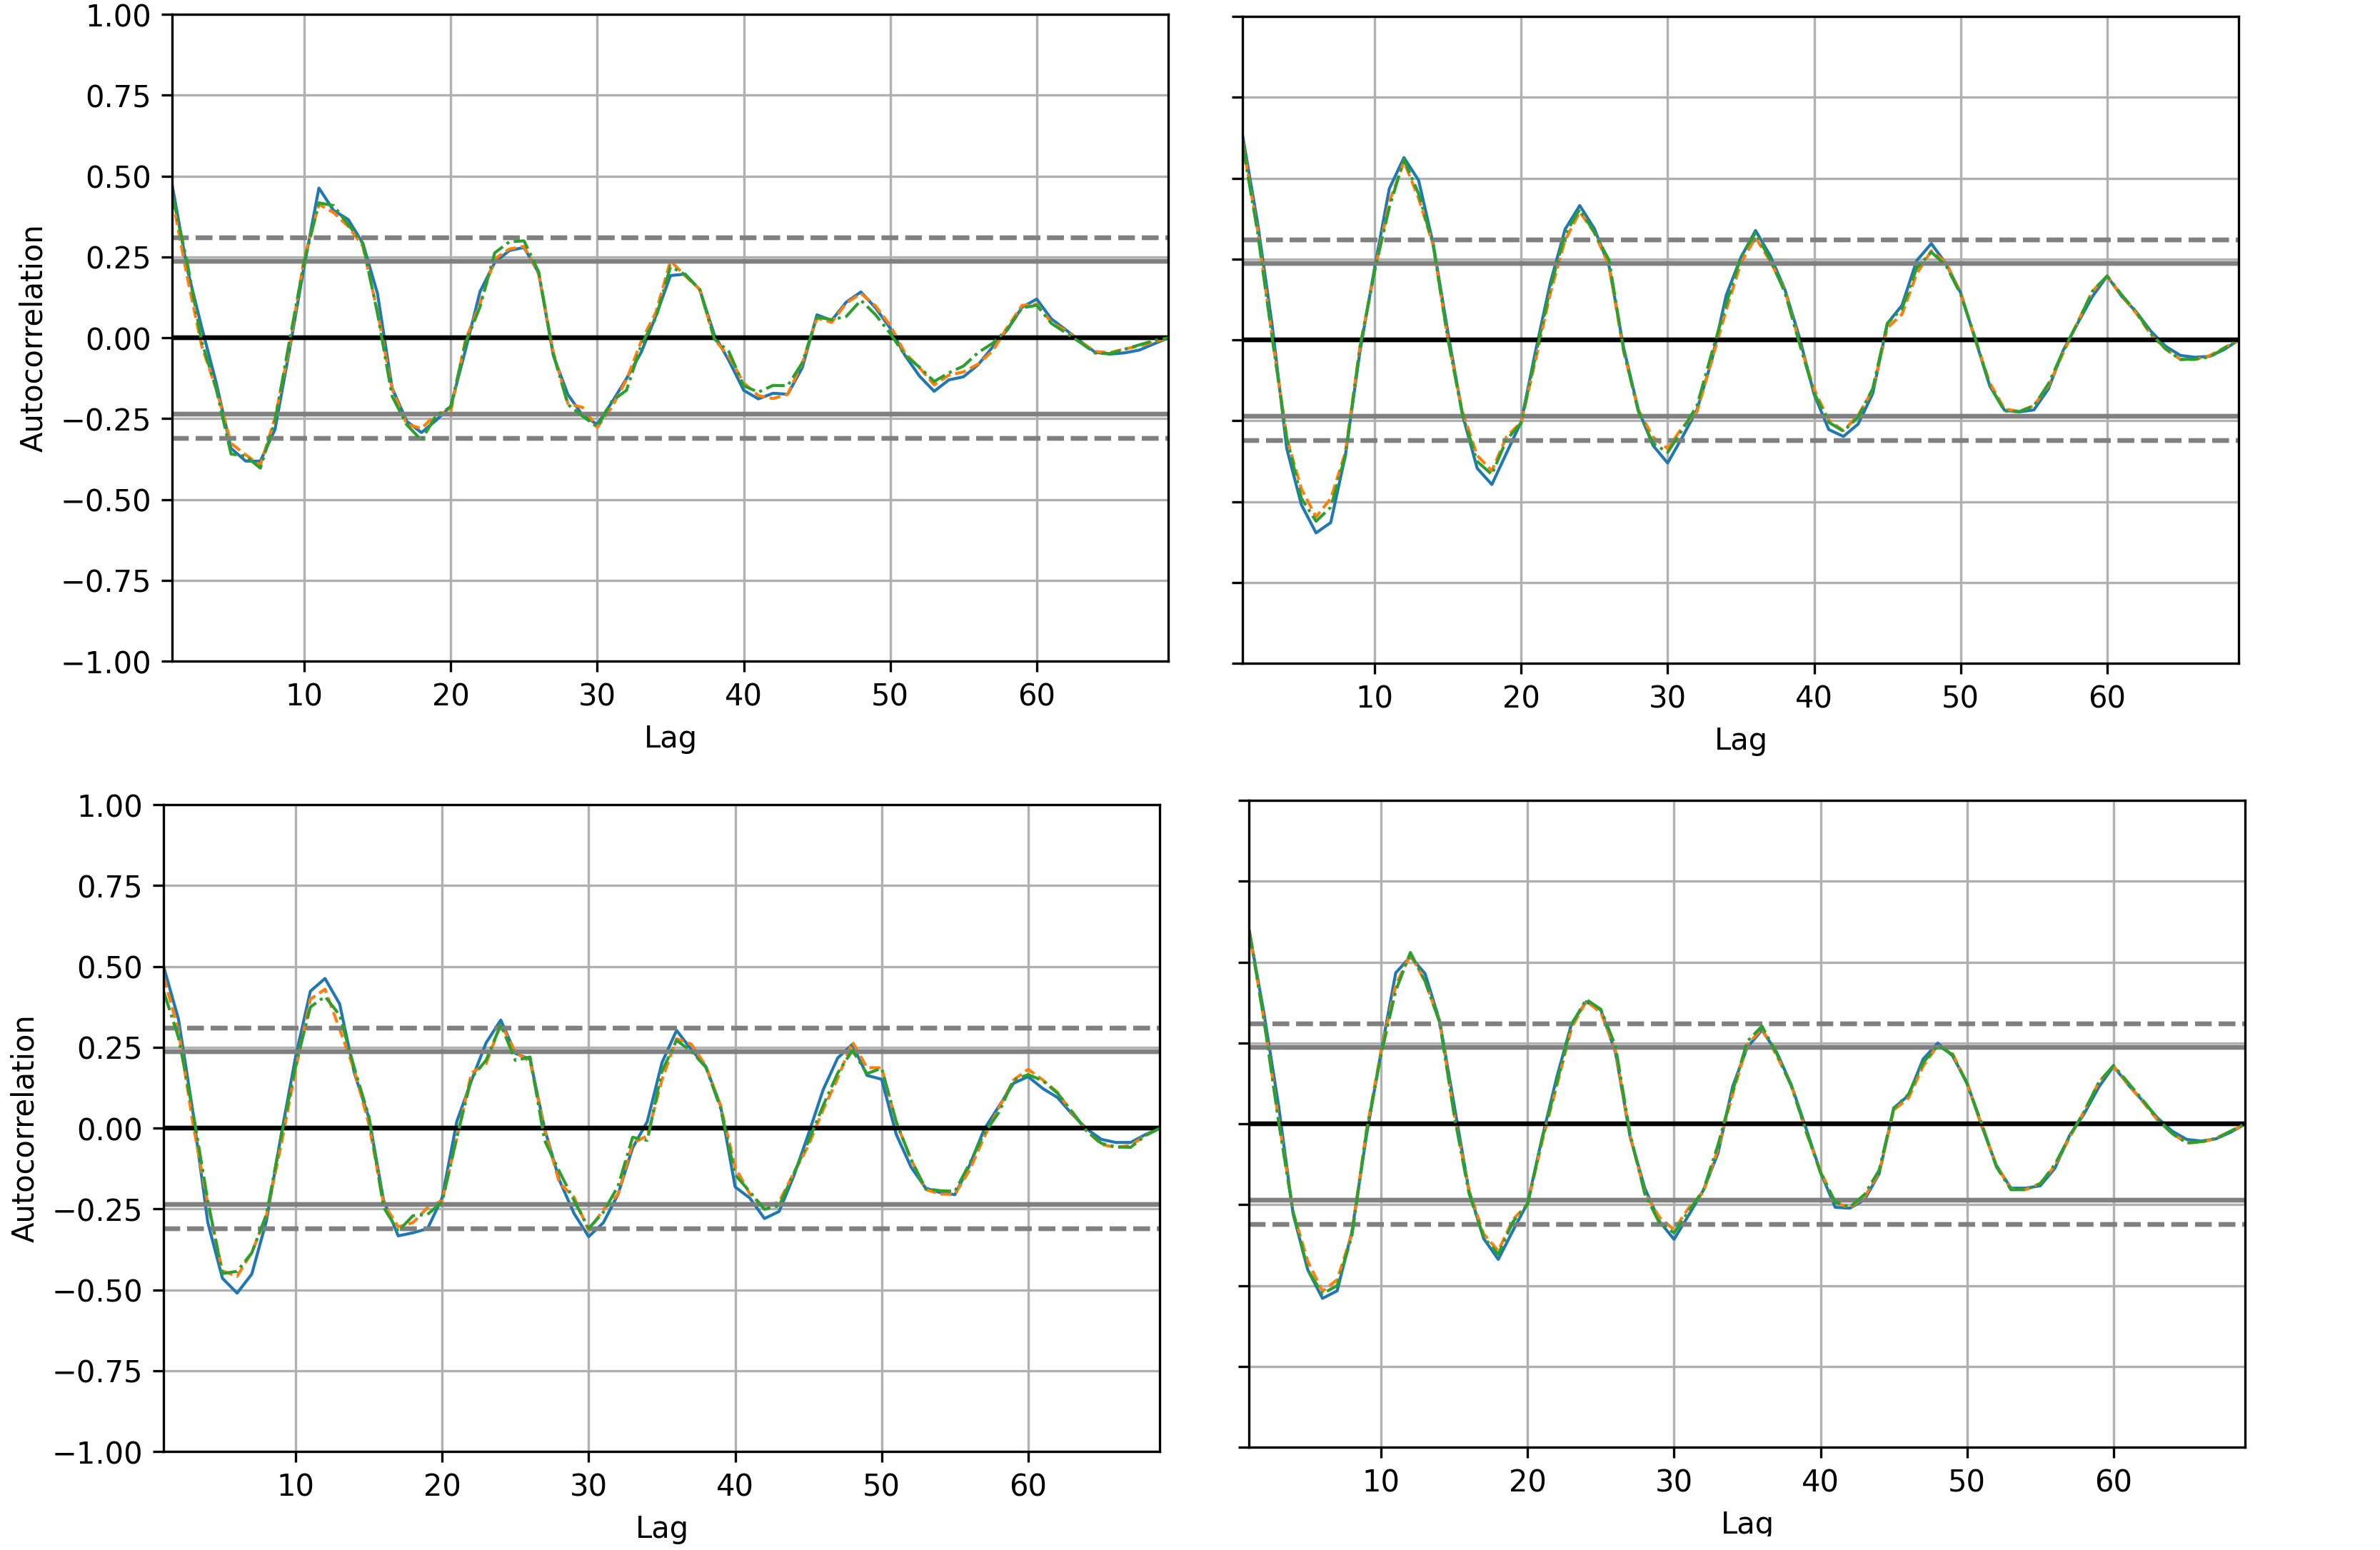
\includegraphics[height=3.5in]{Figures/autocorr_scs.png}
%       \caption{ Funciones de autocorrelación.}
%       \label{resultados_q}
%     \end{center}
%   \end{figure}

% En la figura \ref{autocorrelacion} se muestran las funciones de autocorrelación
% correspondientes a cada una de la subcuencas. Se puede observar que ambos modelos son capaces de captar correctamente 
% la estacionalidad de los datos.



%  \begin{figure}[h!]
%     \begin{center}
%       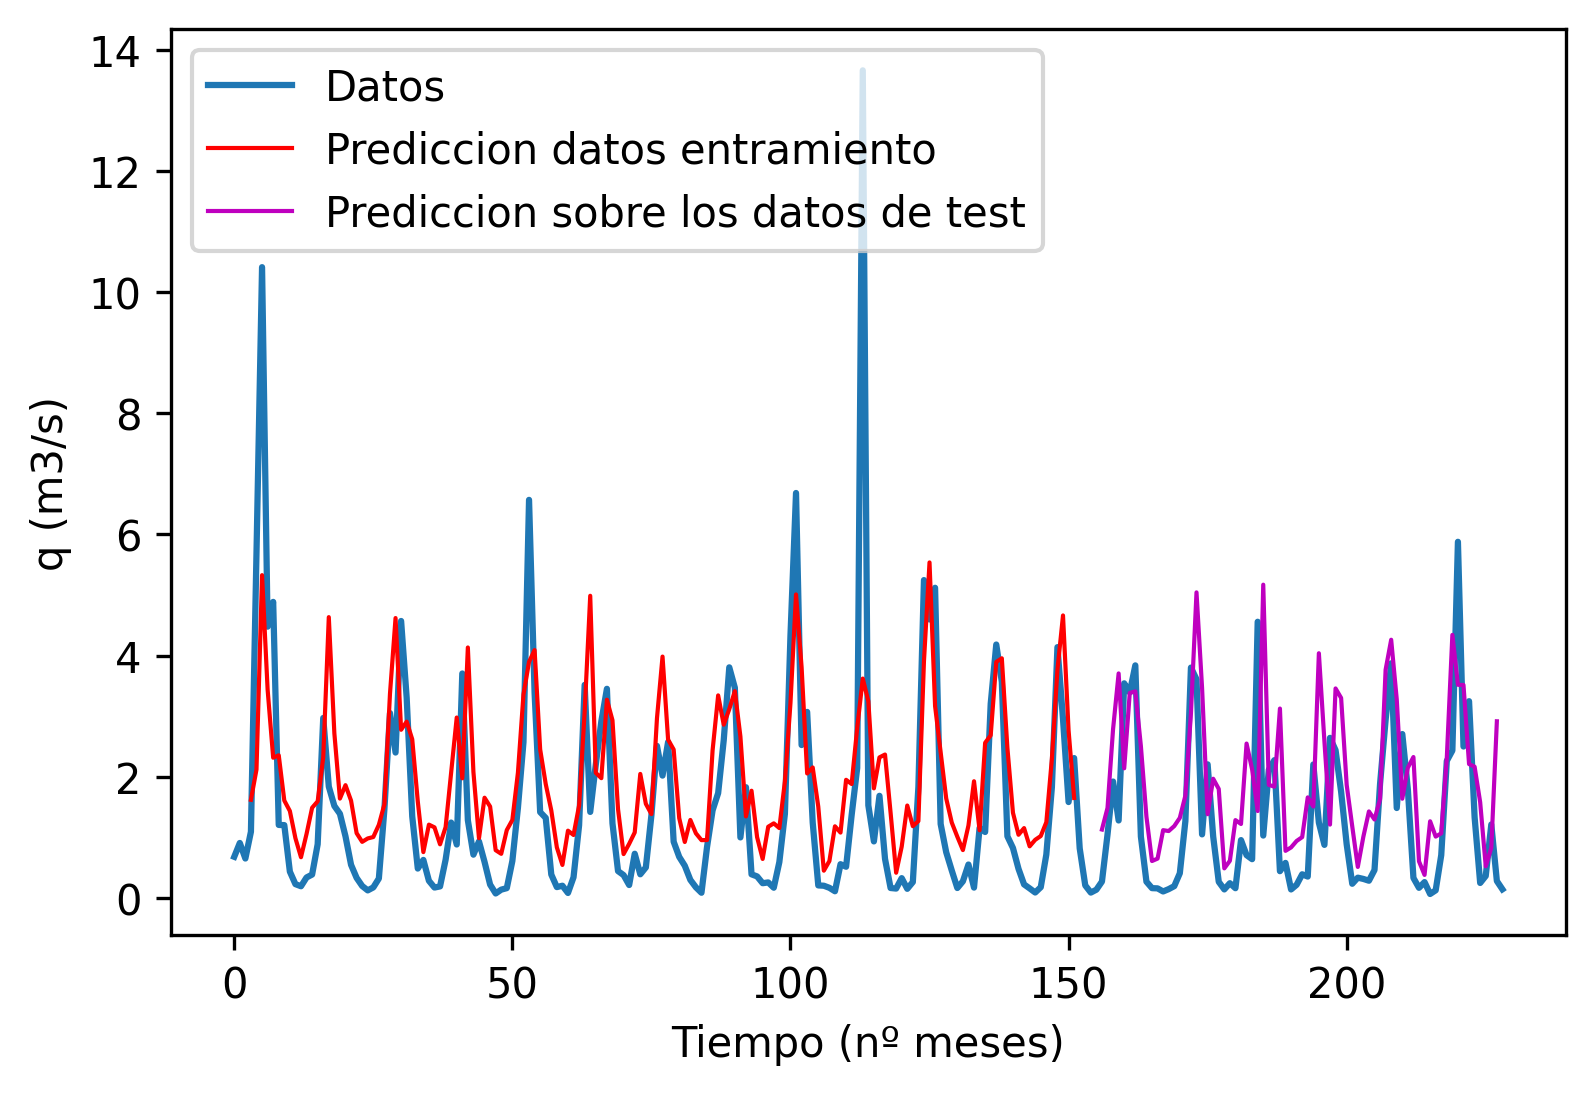
\includegraphics[height=3.in]{Figures/modelo_LSTM_seq.png}
%       \caption{ Resultados del modelo LSTM 3.}
%       \label{result_LSTM3}
%     \end{center}
%   \end{figure}


%   En la figura \ref{result_LSTM3} se muestran los resultados obtenidos con el modelo LSTM3 en todo el rango de datos 
%   para la subcuenca numero 73. En este enfoque, se han predicho los datos de manera secuencial, 
%   para lo cual sólo se ha utilizado la información de las series temporales de los caudales simulados en el
%   conjunto de entrenamiento. Si bien este modelo predice   correctamente la tendencia de los datos, 
%   falla al predecir los valores de los caudales.

  





% %   \begin{figure}[h!]
% %     \begin{center}
% %       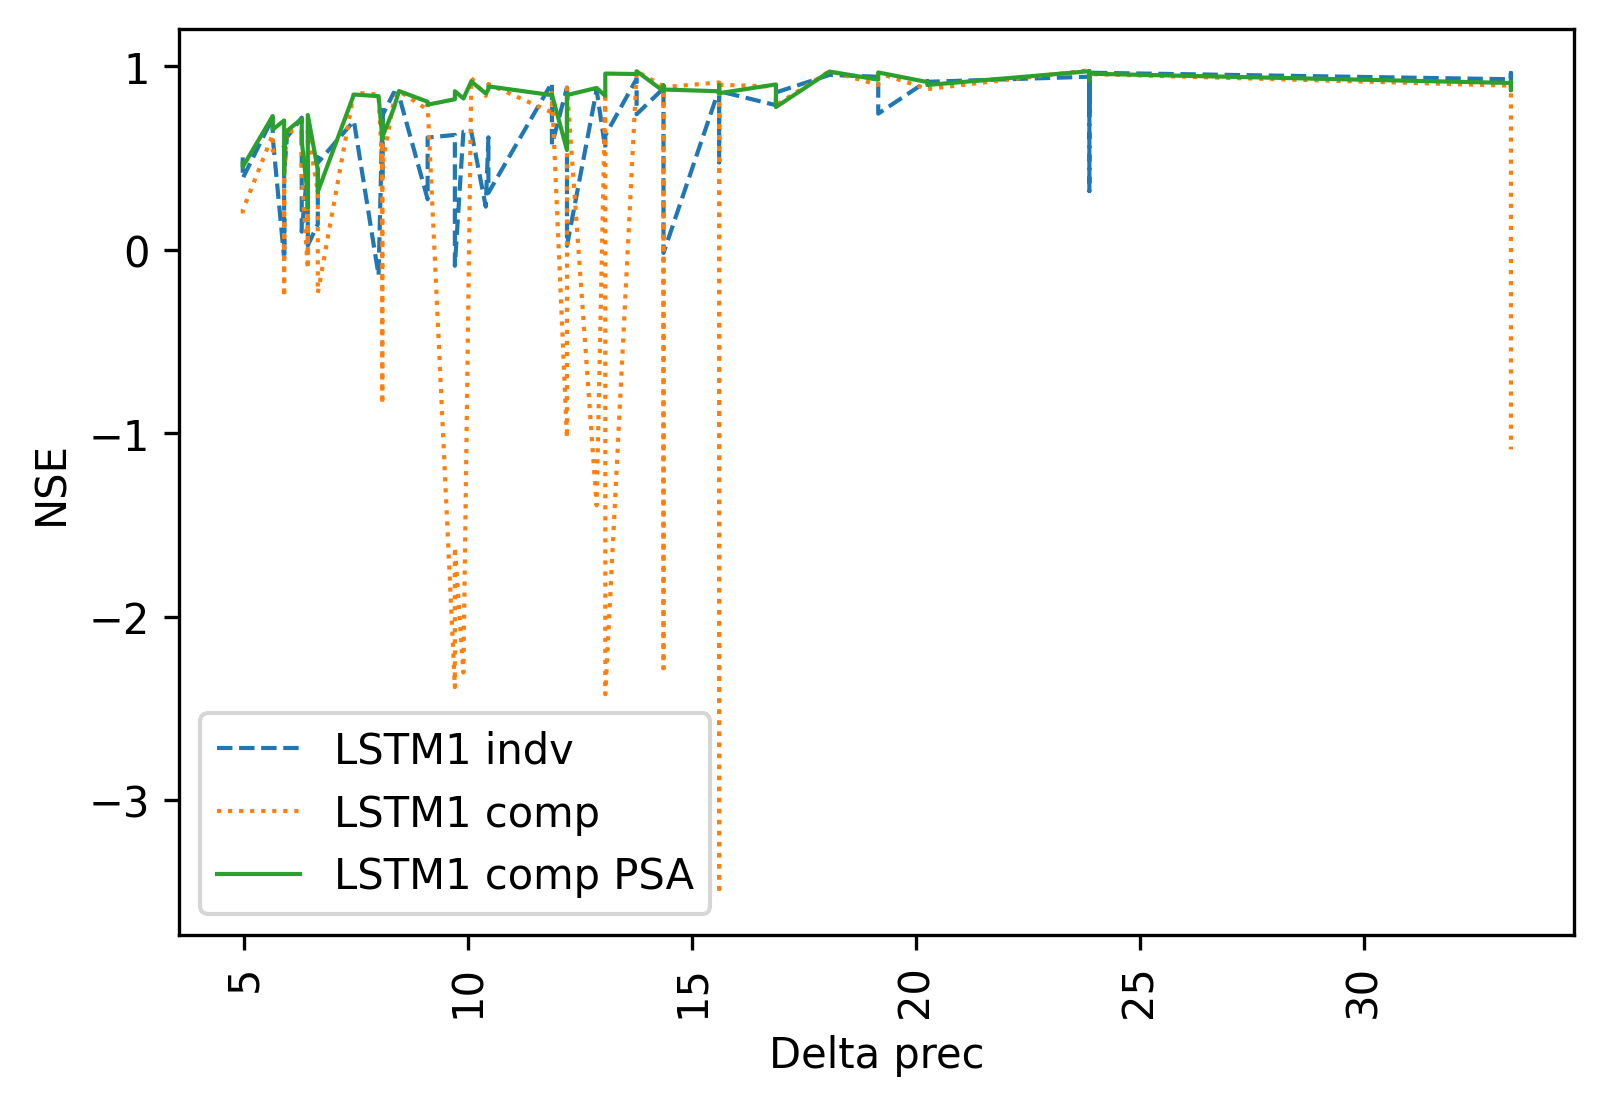
\includegraphics[height=2.in]{Figures/NSEs_Delta prec.png}
% %       \caption{ Modelo LSTM 2}
% %       \label{Red_LSTM2}
% %     \end{center}
% %   \end{figure}

% \section{Resultados finales}

% Con el fin de determinar si los resultados obtenidos utilizando redes neuronales pueden ser utilizados en un problema real 
% de gestión de suministros en una cuenca, se ha alimentado el programa Modsim con los caudales simulados por 
% el modelo hidrológico LEM y los caudales obtenidos por el modelo LSTM1 en el conjunto de test. 
% Se han considerado los diferentes usos del agua por demandas humanas, riego, industriales, etc.
% Los resultados para la salida de la cuenca, se muestran en la figura \ref{modsim}. 
% Se puede apreciar que los resultados son prácticamente iguales.



%   \begin{figure}[h!]
%     \begin{center}
%       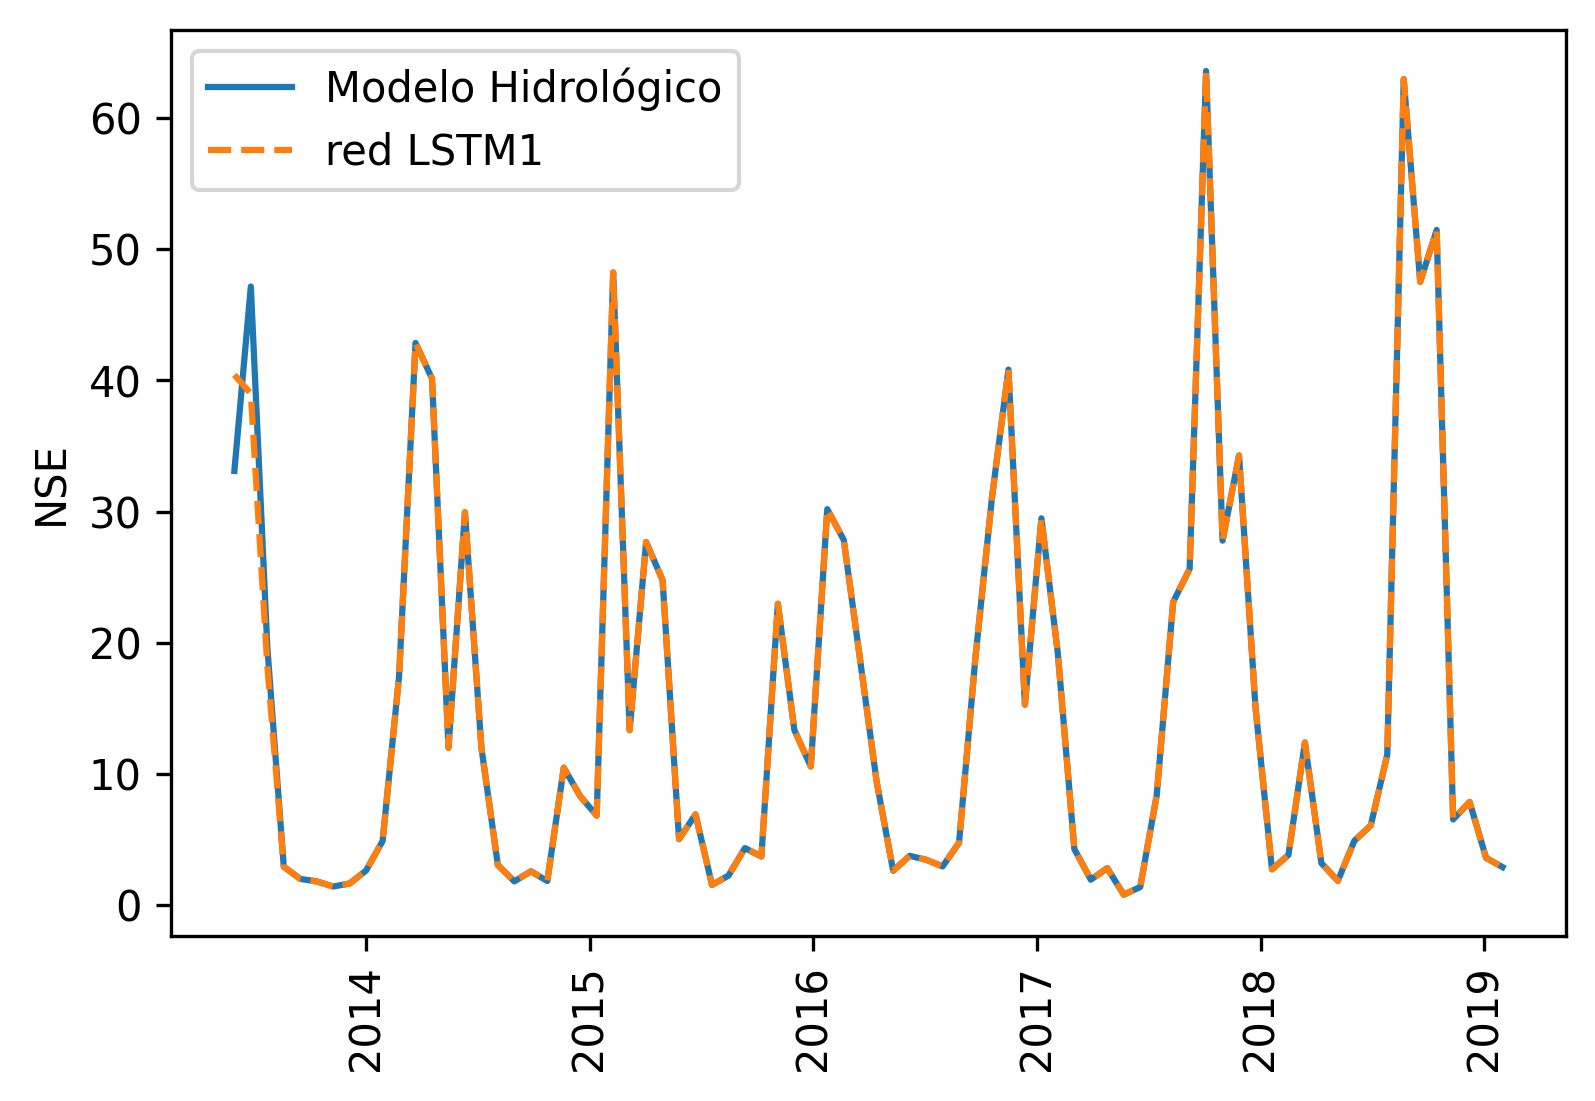
\includegraphics[height=4.in]{Figures/Resultado Modsim.png}
%       \caption{ Resultados finales obtenidos utilizando el software de gestión de recursos Modsim, teniendo en cuenta los usos del agua}
%       \label{modsim}
%     \end{center}
%   \end{figure}


%   % \begin{figure}
% %     \centering
% %     \begin{subfigure}[b]{0.6\textwidth}
% %         \centering
% %         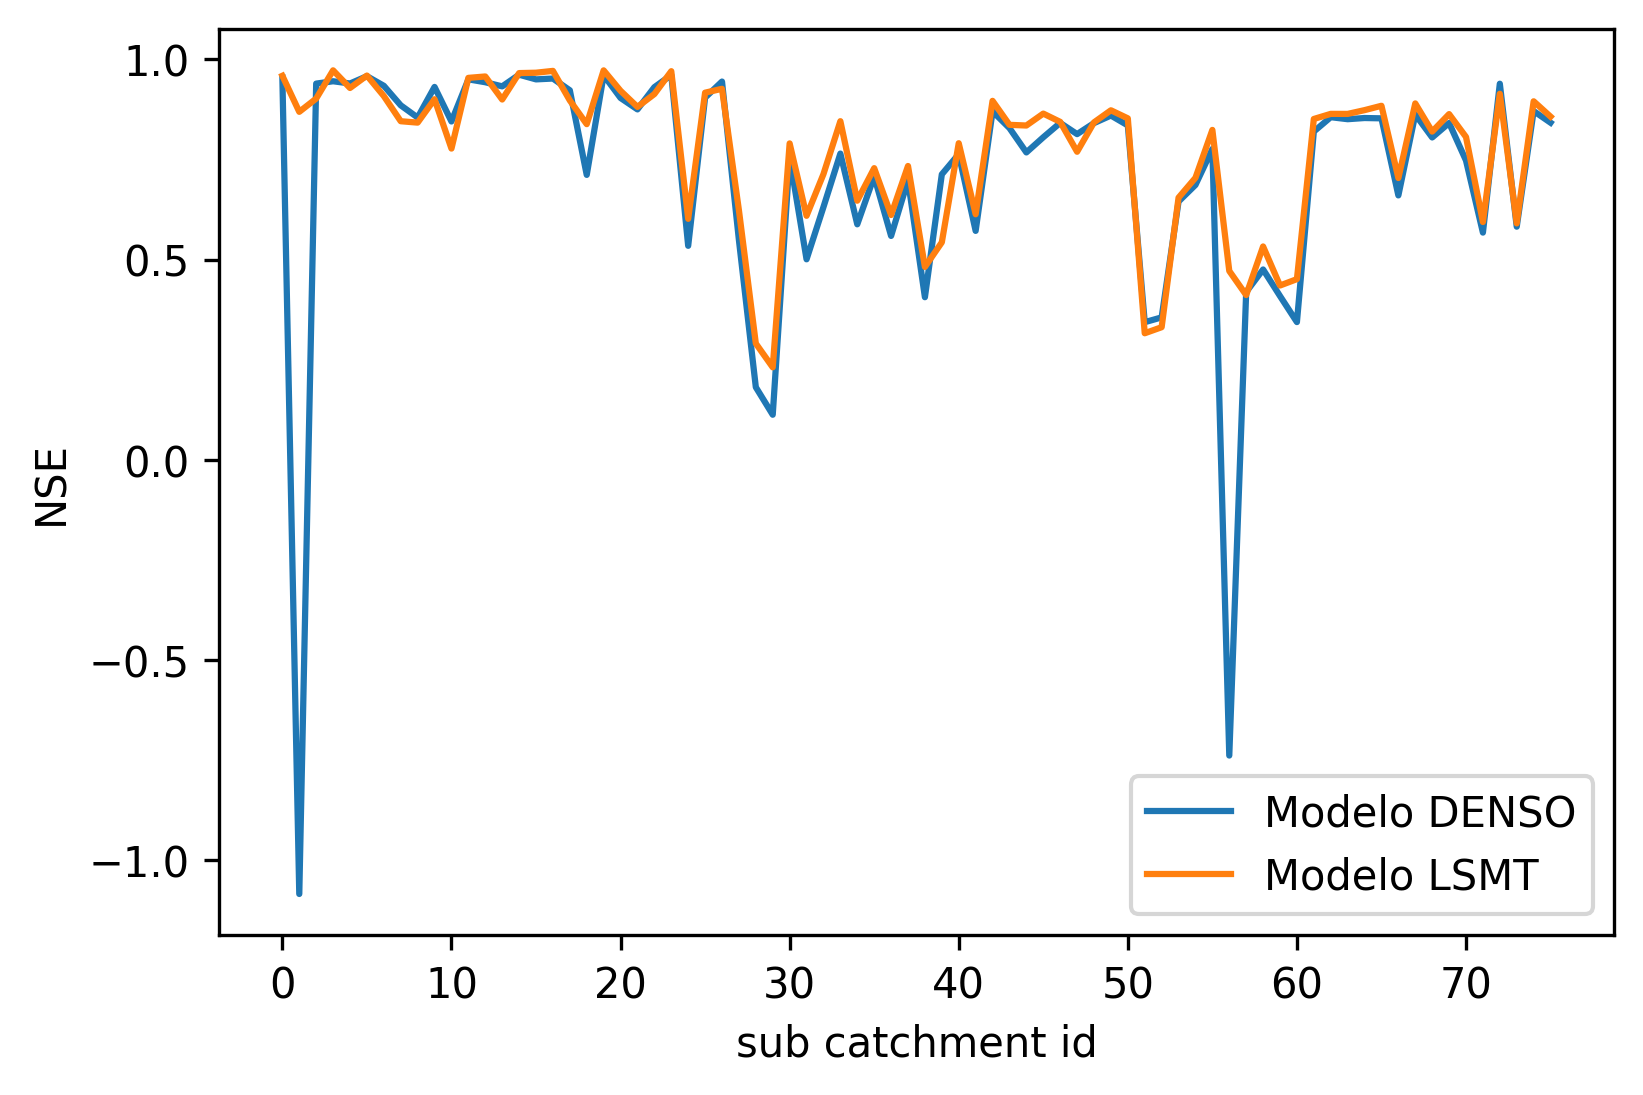
\includegraphics[width=\textwidth]{Figures/comparacion_denso_LSTM_NSE.png}
% %         \caption{}
% %         \label{fig:y equals x}
% %     \end{subfigure}
% %     \hfill
% %     \begin{subfigure}[b]{0.6\textwidth}
% %         \centering
% %         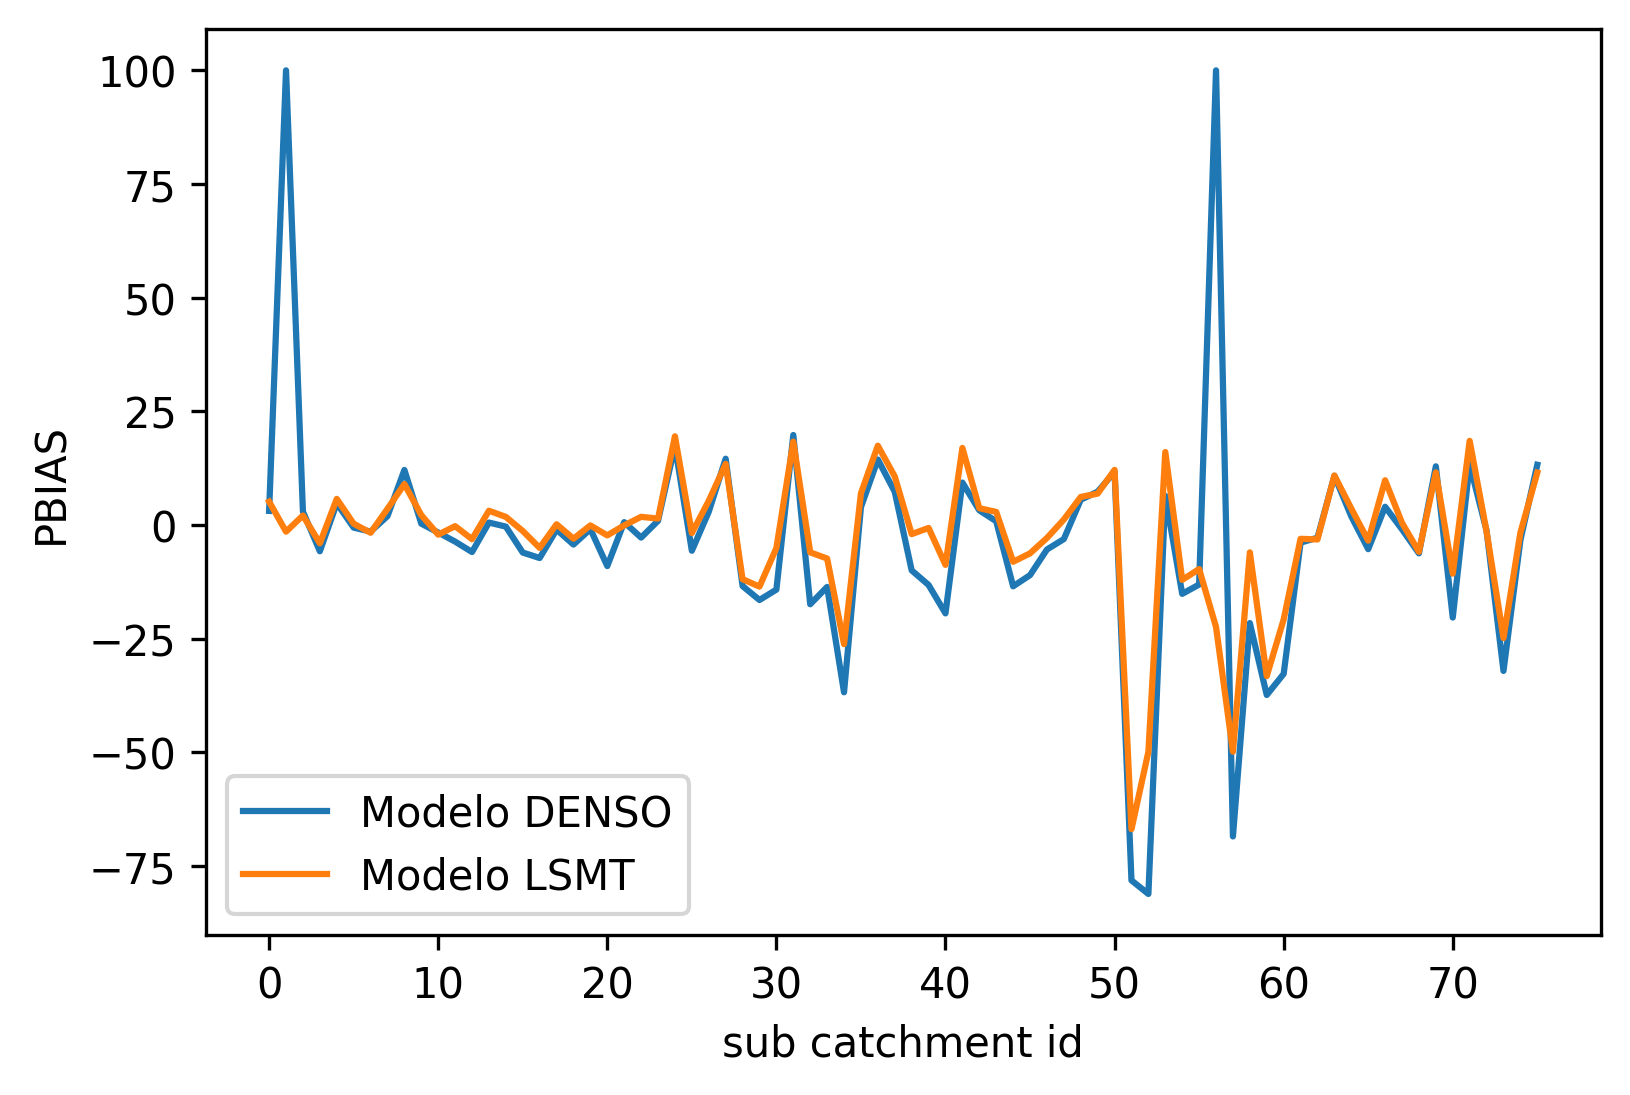
\includegraphics[width=\textwidth]{Figures/comparacion_denso_LSTM_PBIAS.png}
% %         \caption{}
% %         \label{fig:three sin x}
% %     \end{subfigure}
% %        \caption{Three simple graphs}
% %        \label{fig:three graphs}
% % \end{figure}

\chapter{Resultados}
\label{capitulo 3}

En este capítulo se muestran los resultados obtenidos al entrenar los modelos previamente descritos, 
el objetivo es predecir los caudales de descarga naturales en cada una de las sub-cuencas que conforman CHRC para  un evento de 
precipitación dado. 
La performance predictiva de los modelos es evaluada en el conjunto de test, 
en la tabla \ref{hyperres} se muestran los hyper-parámetros utilizados para cada modelo obtenidos
tras realizar la exploración descrita en \ref{cal}.


\begin{table}[]
  \begin{center} 
  \begin{tabular}{|l|l|l|l|l|l|}
    \hline
   Modelo&optimizador &Neuronas & Activación & alpha & reg \\
   \hline
   Denso & rmsprop& 200& relu & 0.0002 &l2, 0.0001  \\
   LSTM1 PCA & rmsprop  &200 & linear &  0.0002  & l2, 0.0001 \\
   LSTM1 loc & adam & 200 & relu & 0.0001 &  l1, 0.0001  \\
   LSTM2 & adam & 200 & relu &  0.001 & l2, 0.0000001 \\
  
   \hline

  \end{tabular}
  \caption{ Hyper parámetros utilizados en los diferentes modelos.}
  \label{hyperres}
\end{center}
  \end{table}

\section{Validación de los modelos}


 \begin{figure}[h!]
   \begin{center}
     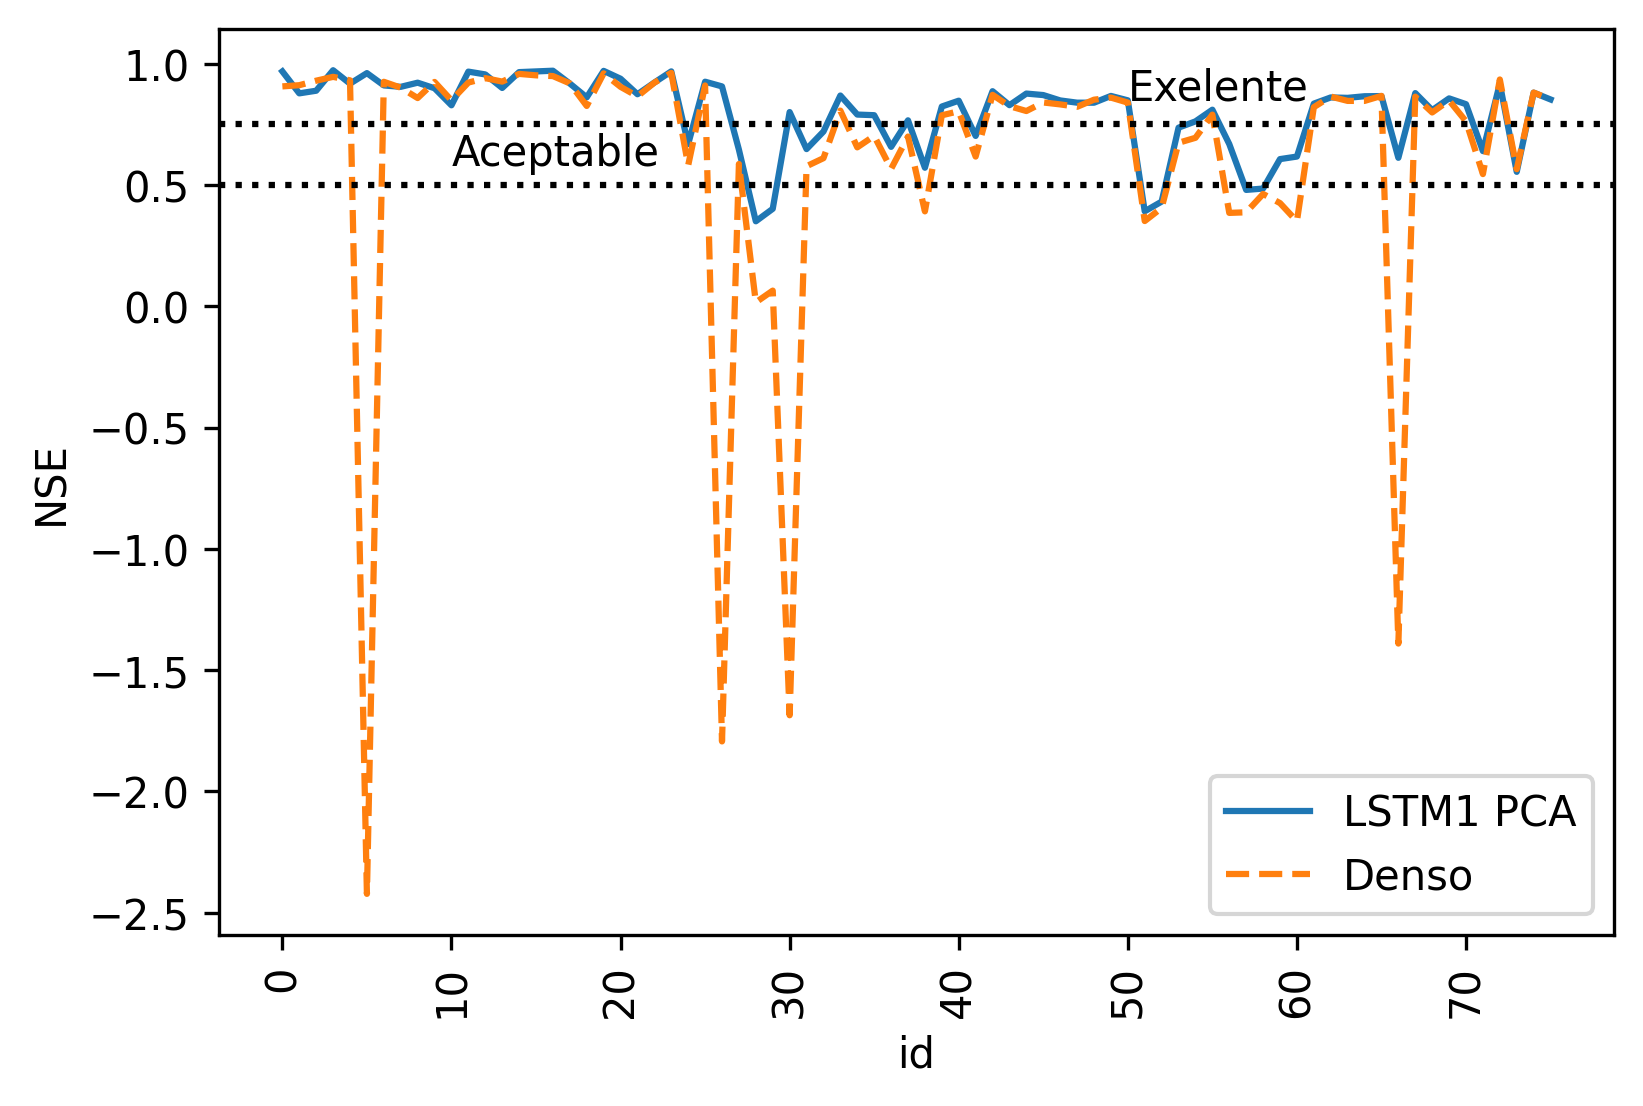
\includegraphics[height=3.in]{Figures/NSE/NSEs_LSTM1s_PCA.png}
     \caption{ Valores obtenidos para el coeficiente NSE a lo largo de toda la cuenca con los modelos denso
     y LSTM1 entrenado con PCAs.}
     \label{NSE1}
   \end{center}
 \end{figure}


Como se ha mencionado en la sección \ref{sectNSE}, se ha utilizado el coeficiente de Nash-Sutcliffe para
validar los modelos y hacer un análisis un poco más profundo sobre cómo es su performance en los diferentes puntos
de la cuenca. En la figura \ref{NSE1} se muestran los valores obtenidos 
de NSE para todas las sub-cuencas de Chambo considerando el modelo denso y el modelo LSTM1 entrenado de manera global 
en el espacio de las componentes principales. Las líneas horizontales muestran los umbrales correspondientes a 
ajustes excelentes y aceptables. 

El modelo LSTM1 posee una mejor performance general a lo largo de toda la cuenca, 
en este caso se  puede considerar que el ajuste para el 68$\%$ de las sub-cuencas es excelente, 
mientras que el 11$\%$ de los ajustes son buenos y el 16$\%$  aceptables. 
Por otro lado, si bien la performance general del modelo denso es buena (el 68$\%$ es mayor a $0.65$), 
el porcentaje de fallos asciende al 13$\%$. Se puede observar que en las subcuencas con ids 5, 26, 31 y 66 el coeficiente NSE adquiere 
valores negativos, mientras que el modelo LSTM1 realiza muy buenos ajustes.
La mejor performance del modelo LSTM1 se debe a que las celdas de memoria permiten una interpretación a lo largo del eje del tiempo de 
los diferentes procesos que ocurren en cada una de las cuencas, lo que permite captar más información sobre la relación entre
eventos de precipitación y descarga. 


\begin{figure}[h!]
  \begin{center}
    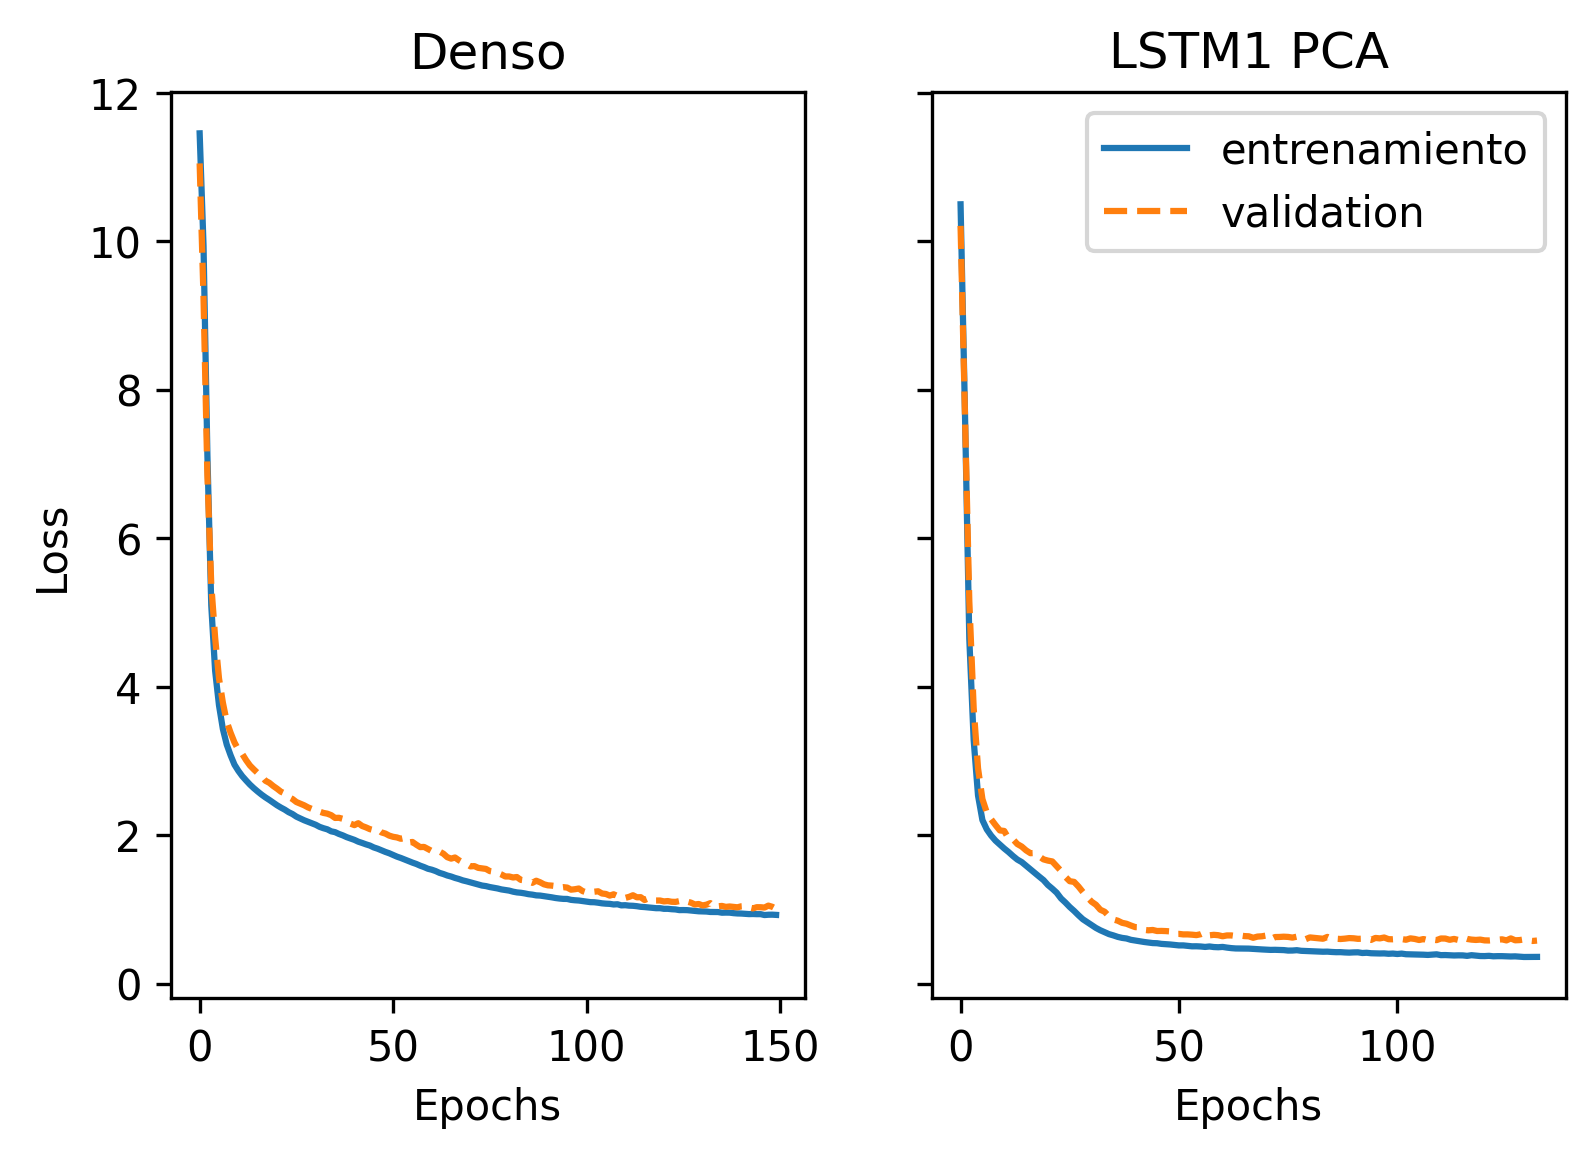
\includegraphics[height=3.in]{Figures/loss/comp_loss.png}
    \caption{ Evolución de la función de loss en los conjuntos de entrenamiento y validación para los modelos denso y
    LSTM1 con PCAs.}
    \label{losscomp}
  \end{center}
\end{figure}

En la figura \ref{losscomp} se muestran los valores de la función de loss obtenidos en cada época o iteración durante el entrenamiento
de los modelos denso y LSTM1 PCA.  Durante el entrenamiento se ha dividido el conjunto de datos de manera que el 
85$\%$ de los mismos han sido utilizados para entrenar el modelo y el 15$\%$ restante para validarlo y así evitar el sobre ajuste
monitorizando la evolución del loss. Además se ha implementado el callback "\textit{early sttoping}" que 
interrumpe la ejecución cuando el loss en el conjunto de validación comienza a aumentar.

Si se comparan ambos modelos, podemos observar que
en el modelo LSTM1 PCA aprende más rápido ya que en aproximadamente 50 épocas el valor de loss alcanza su valor de equilibrio, 
en el caso del modelo denso, esto ocurre luego de 150 épocas. Por otro lado, y en concordancia con los resultados
arrojados por el coeficiente NSE, el valor final del loss en el modelo LSTM1 PCA (entrenamiento: 0.3587 , validación: 0.5787)
es menor que en el modelo denso (entrenamiento: 0.9245 validación: 1.0060) los que indica un mejor ajuste global. 


  \begin{figure}[h!]
    \begin{center}
      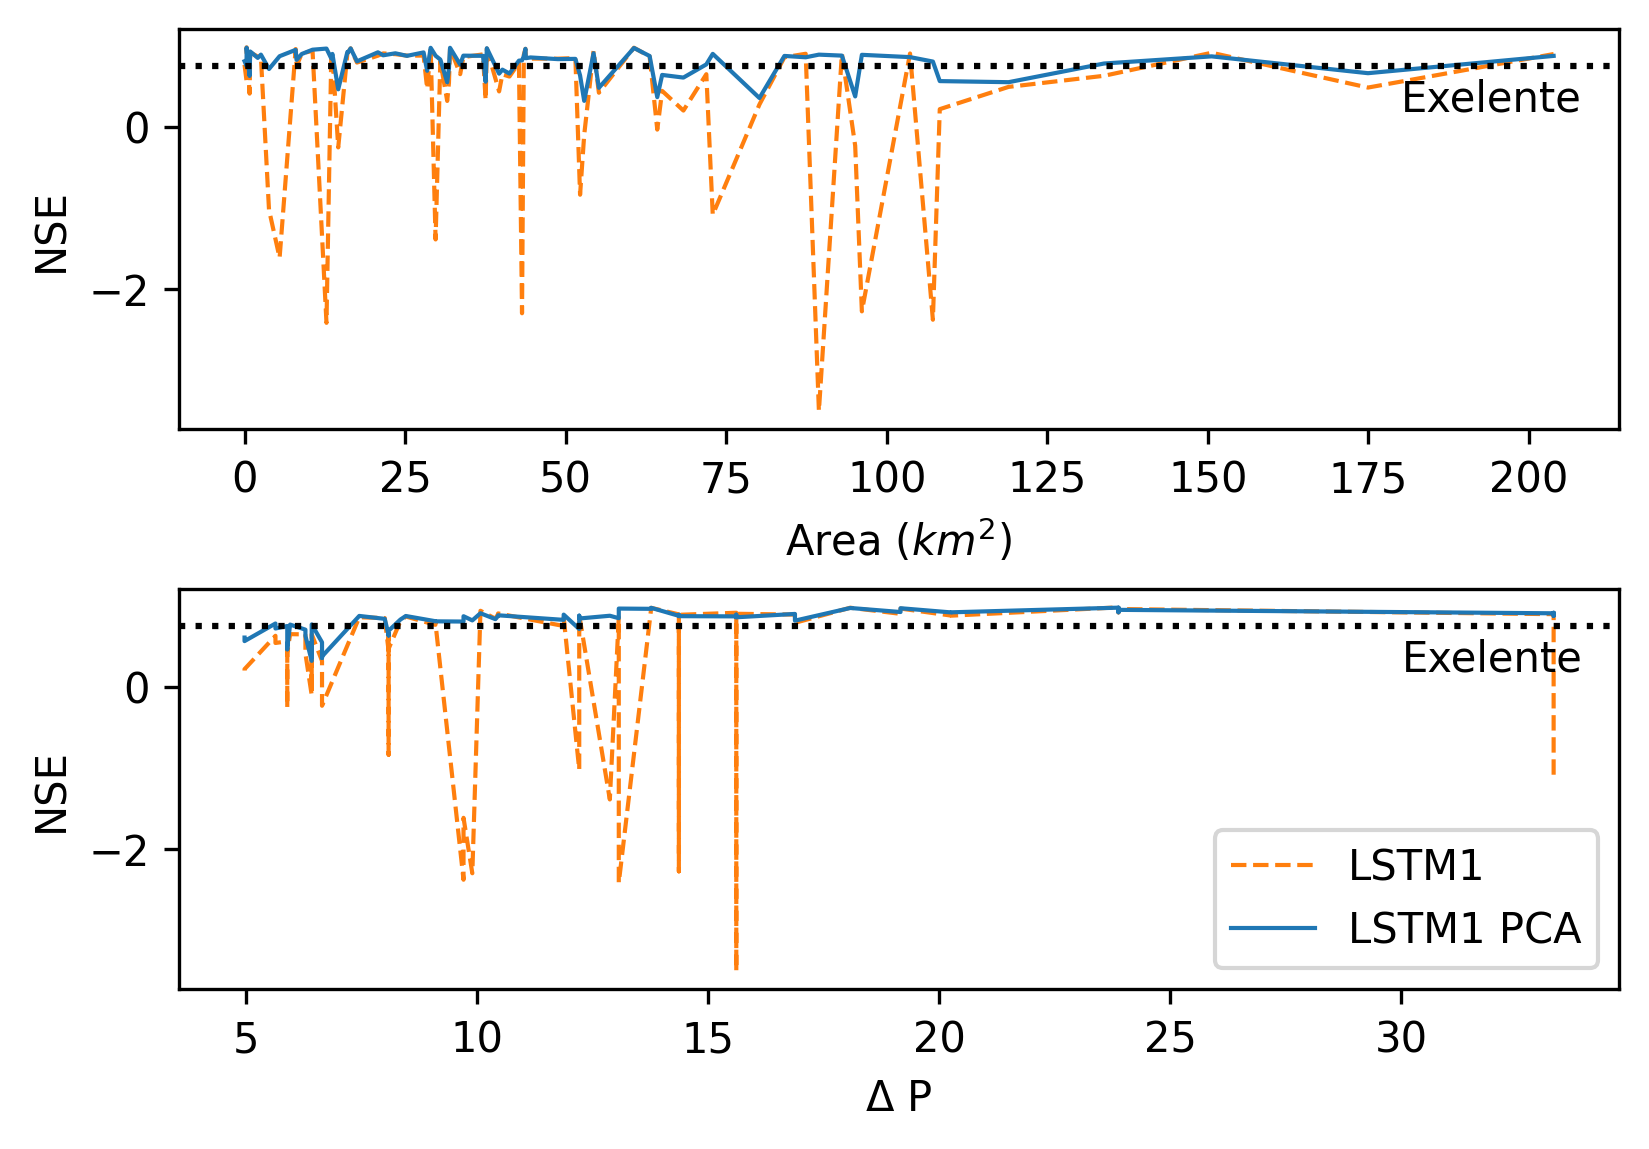
\includegraphics[height=3.5in]{Figures/NSE/comp_NSE_consinPCA.png}
      \caption{ Evolución del coeficiente NSE en función del área (panel superior) y la variación de precipitación 
      (panel inferior) para los modelos LSTM1 con y sin PCAs.}
      \label{NSEs_Area_prec}
    \end{center}
  \end{figure}


En la figura \ref{NSEs_Area_prec}, se muestra la comparación entre los valores de NSE obtenidos para el modelo LSTM1 con PCAs 
(curva continua) y sin PCAs (curva a rayas) en función del área de la cuenca (panel superior) y de la variación de precipitación 
(panel inferior). Los resultados obtenidos cuando consideramos las 288 características
de entrada muestran una gran fluctuación de los valores de NSE y en general peores predicciones. 
Una razón por la que las componentes principales funcionan mejor puede deberse a que éstas agregan la información proveniente de 
todo el dominio del espacio predictor \cite{Manu}. En línea con este argumento, en estas figuras también se puede observar que el 
área de las sub-cuencas y la variación de precipitación son factores relevantes que condicionan la calidad de los ajustes. 
El modelo que no incluye componentes principales  tiende a fallar más en las cuencas pequeñas ($Area  < 120~km^2$) y 
áridas  ($\Delta P < 20~mm/d$). Esto puede deberse a que en estos casos los 
valores de la precipitación y caudales son más pequeños y el loss es en general menor  que el loss para una sub-cuenca con
una descarga grande. Esto último provoca que el modelo deje de aprender demasiado pronto y se genere un
un sobre peso para las sub-cuencas más grandes y húmedas mientras que la performance en las 
más pequeñas y áridas disminuye \cite{Kratzert}.

\begin{figure}[h!]
  \begin{center}
    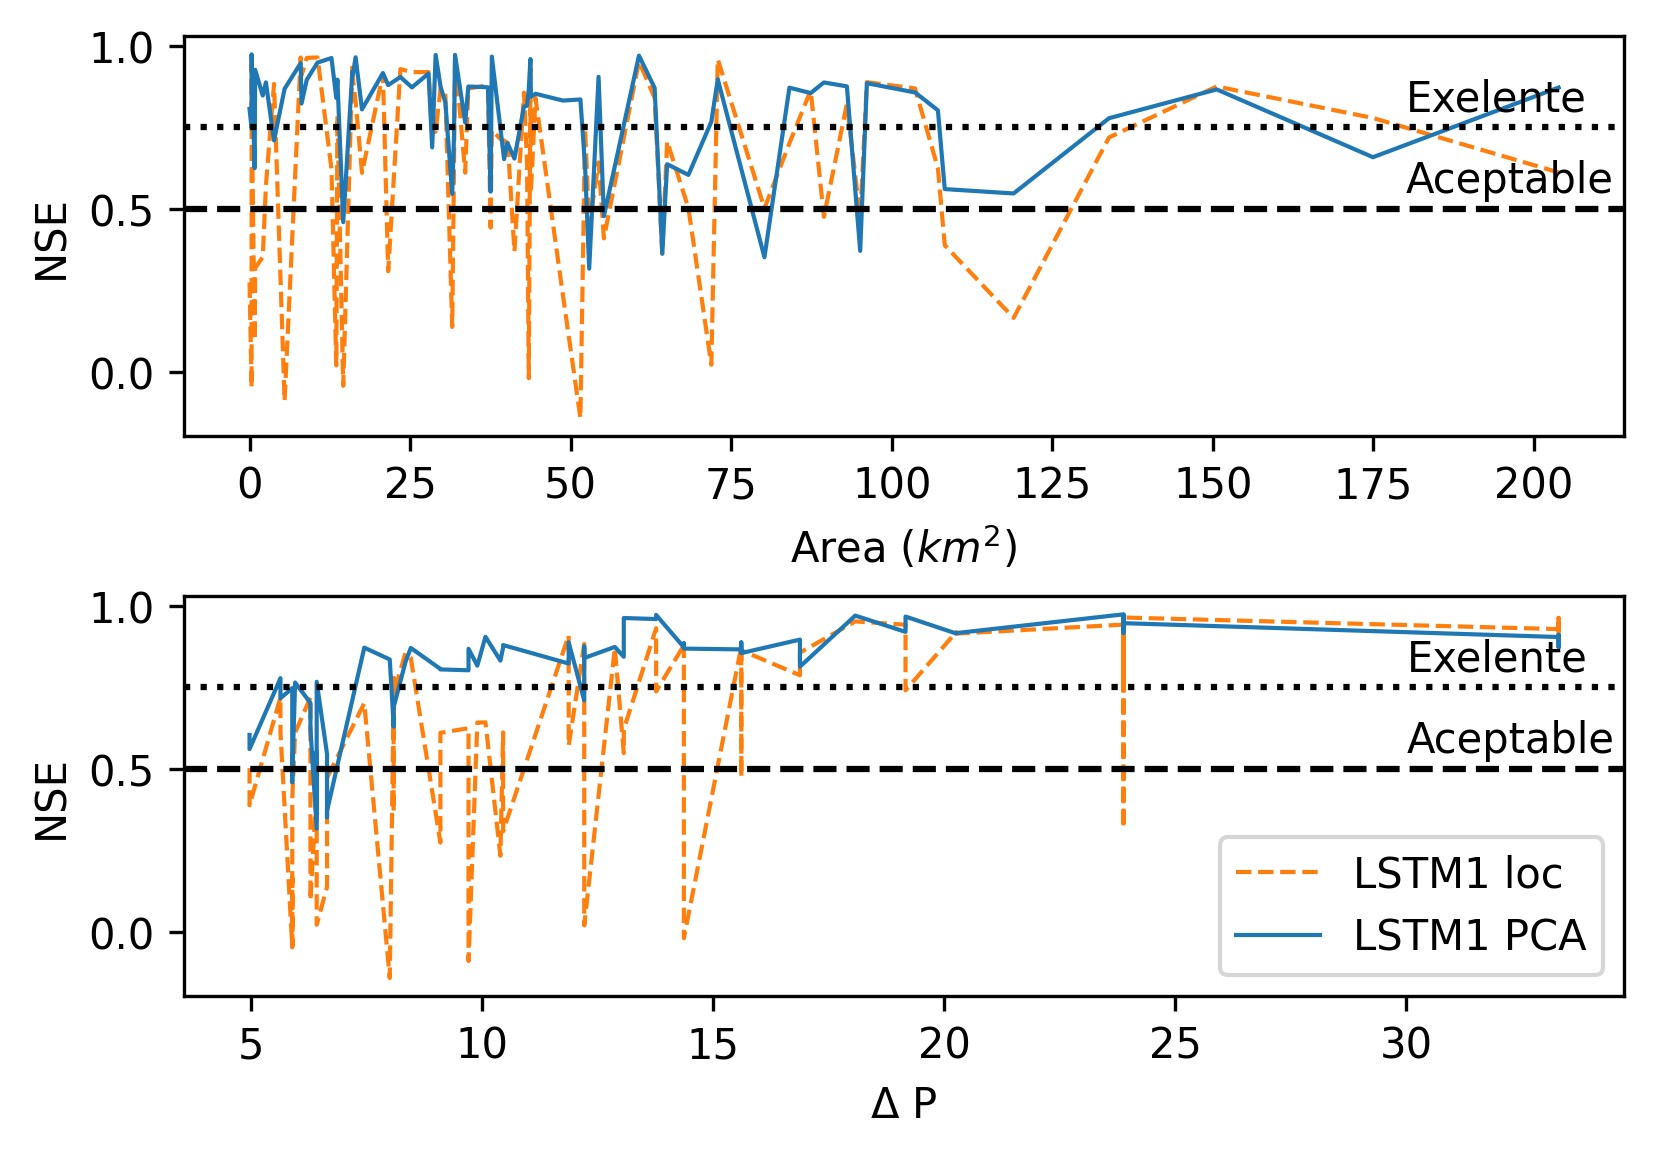
\includegraphics[height=3.5in]{Figures/NSE/comp_NSE_consinPCA2.png}
    \caption{ Evolución del coeficiente NSE en función del área (panel superior) y la variación de precipitación 
    (panel inferior) para los modelos LSTM1 con PCAs y LSTM1 entrenado localmente.}
    \label{NSE3}
  \end{center}
\end{figure}




% the MSE from a basin with low average discharge (e.g., smaller, arid basins) is generally smaller than the MSE from a basin 
% with high average discharge (e.g., larger, humid basins). We need an objective function that does not depend on basin-specific 
% mean discharge so that we do not overweight large humid basins (and thus perform poorly on small, arid basins).

Este efecto es también visible cuando entrenamos el modelo LSTM1 de manera local,
como puede verse en la figura \ref{NSE3} en la mayoría de los casos, la performance del modelo global  es 
mejor que la del modelo local. Este resultado se encuentra alineado con estudios 
que demuestran que los modelos LSTM entrenados en un gran número de sub-cuencas son capaces de vincular Las
características de las mismas para aprender un modelo global que a su vez es capaz de reflejar  
explícitamente las similitudes y diferencias de las cuencas a nivel local  \cite{Kratzert}. 


\begin{figure}[h!]
  \begin{center}
    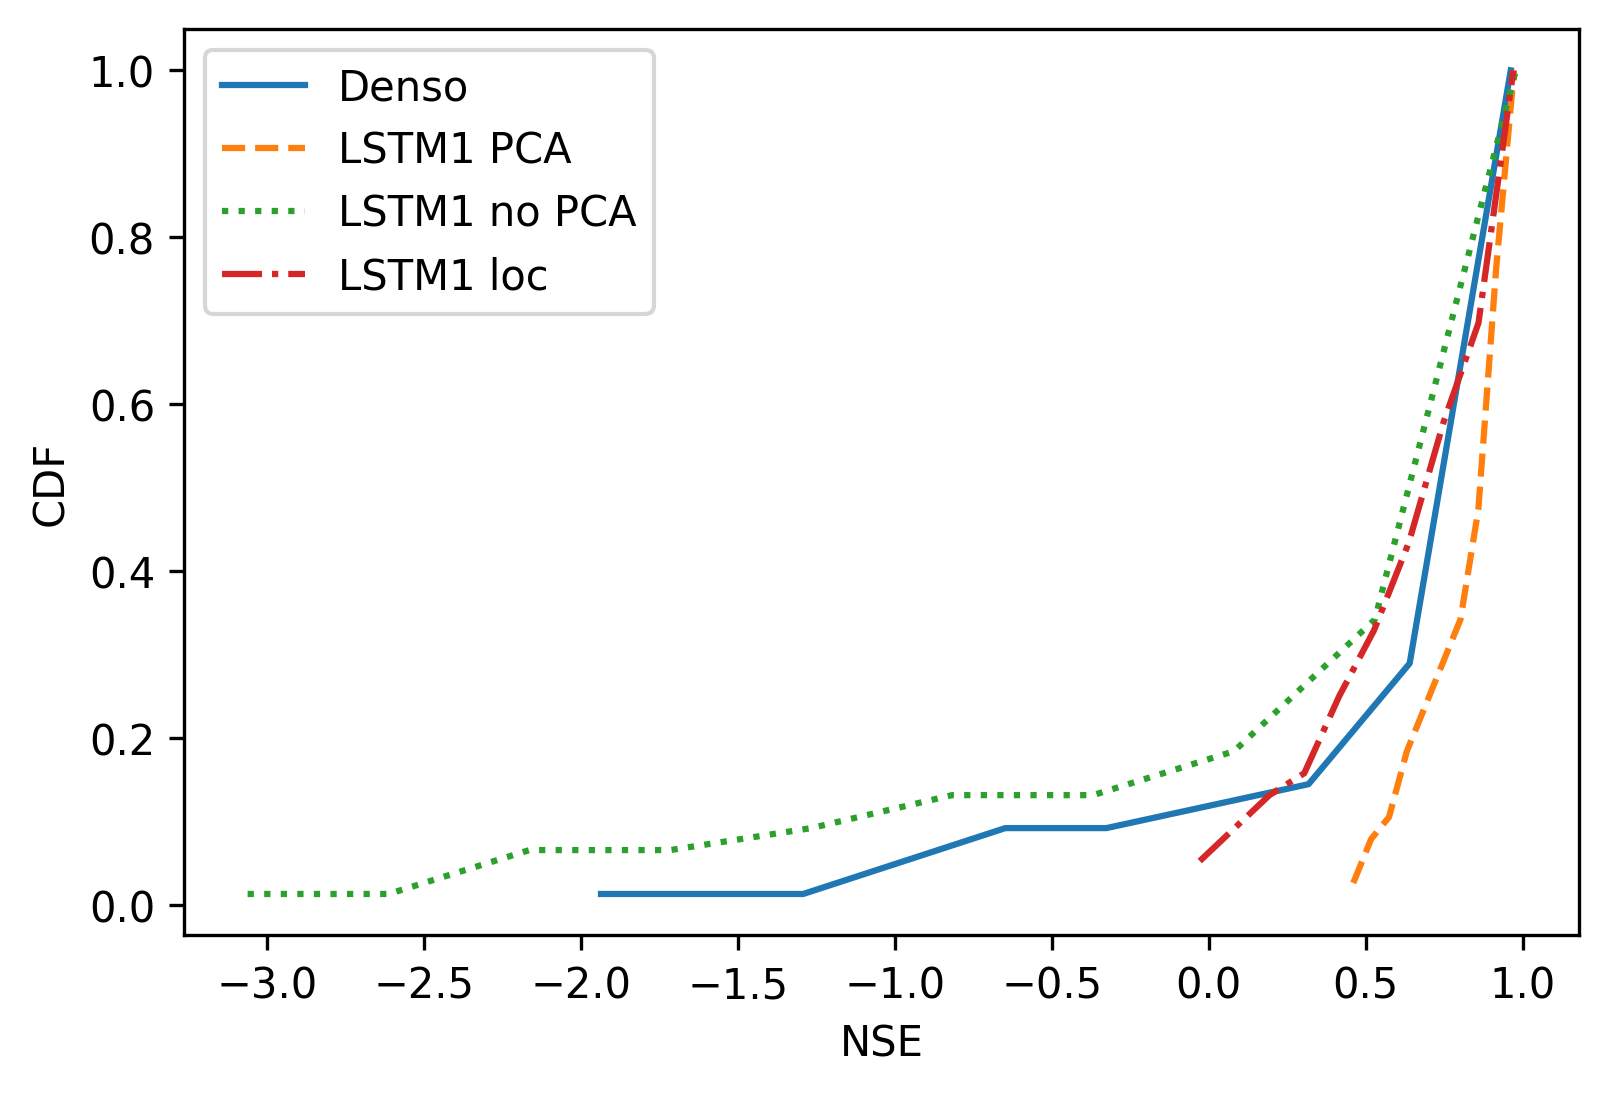
\includegraphics[height=3.5in]{Figures/NSE/CDF.png}
    \caption{ Función de distribución acumulada para todos los modelos de ANNs a lo largo de todas las sub-cuencas de CHRC.}
    \label{CDF}
  \end{center}
\end{figure}

En la figura \ref{CDF}, se muestra una comparación de la función de distribución acumulada para todos los modelos sobre las 76 sub-cuencas de CHRC.
En esta figura se puede ver claramente que el modelo que mejor funciona en general es el LSTM1 PCA. El modelo denso es el segundo mejor en algunos
sectores y el que muestra la peor performance en toda la cuenca es el modelo que usa el espacio predictor sin hacer el análisis de componentes principales.

\section{Predicción de los caudales naturales}


\begin{figure}[h!]
  \begin{center}
    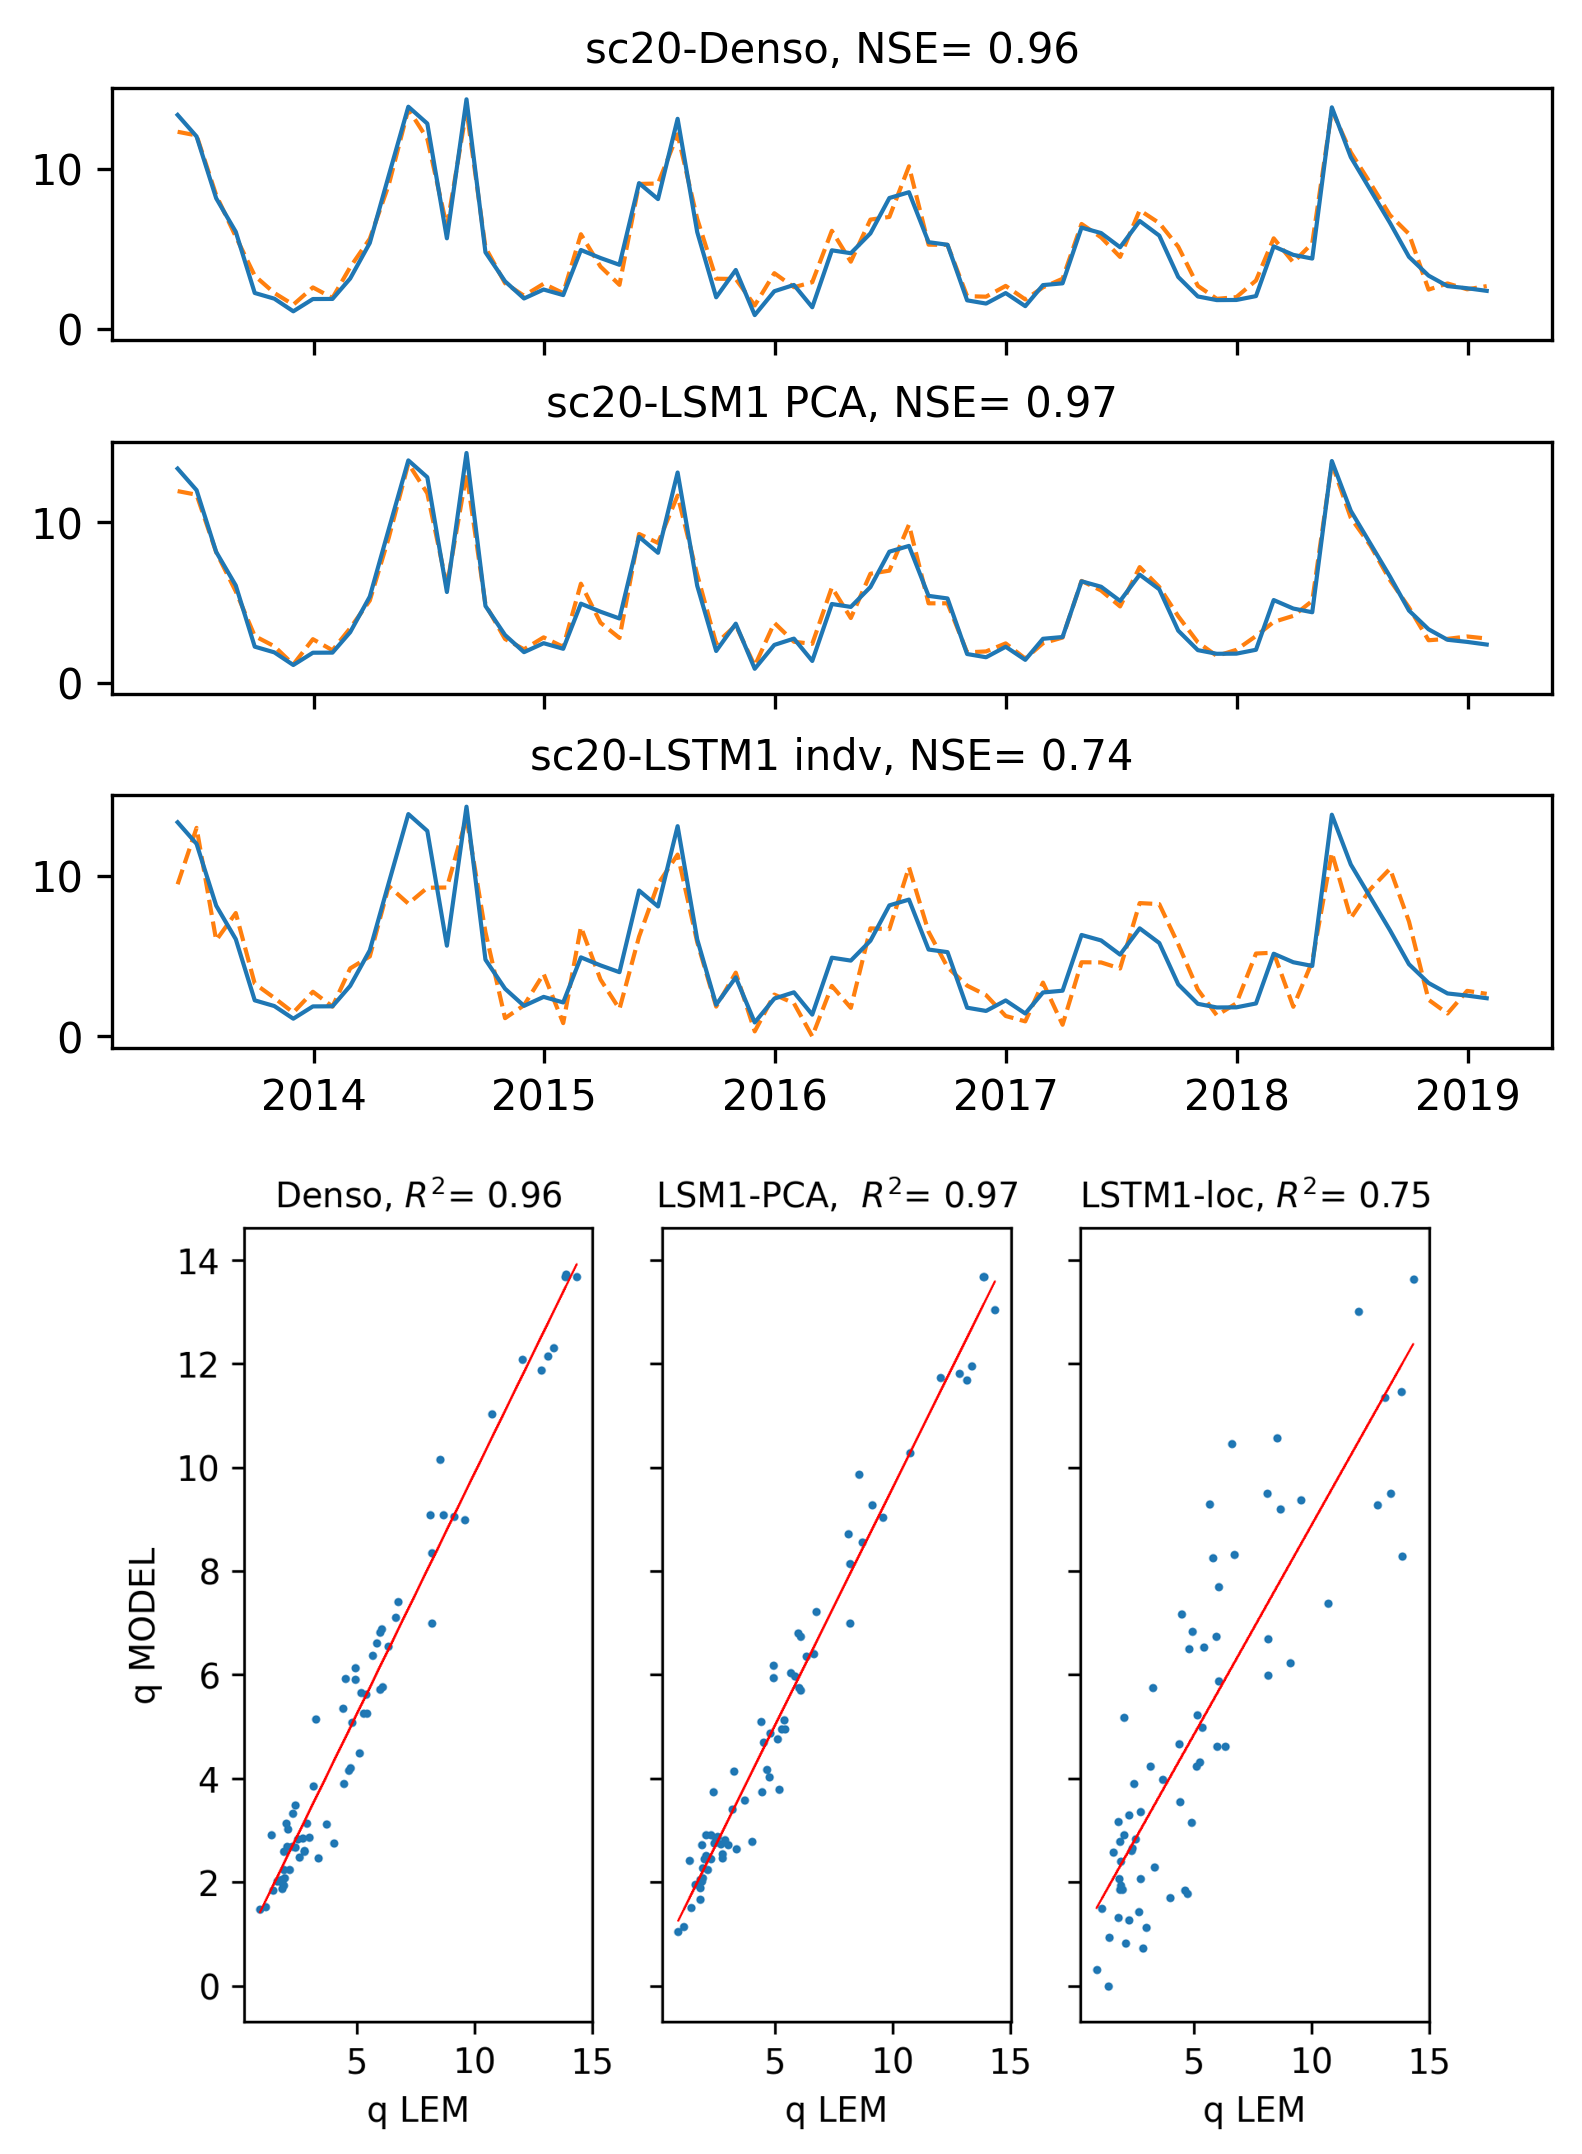
\includegraphics[height=6.in]{Figures/comp_grilla/resultados_sc20}
    \caption{ Predicciones del caudal de descarga obtenidos con los modelos Denso, LSTM1 con PCAs y LSTM1 local en la subcuenca 
    con id 20. En los
    paneles inferiores se muestran los grados de ajuste correspondientes.}
    \label{alcomp20}
  \end{center}
\end{figure}



En las figuras \ref{alcomp20} se muestran  los resultados obtenidos para los caudales en la sub-cuenca con id 20
y los grados de ajustes correspondientes obtenidos con los diferentes modelos.
Las curvas continuas son los valores simulados con el modelo MELCA y las curvas a rayas son los valores predichos 
con los modelos denso, LSTM1 PCA y LSTM1 loc en el conjunto de test. En este caso la performance de los modelos
LSTM1 PCA y denso es excelente, con valores de NSE iguales a 0.97 y 0.96, respectivamente, 
mientras que el modelo entrenado localmente es un poco más baja. Como se ha explicado en sesiones anteriores, los
modelos entrenados de manera global con componentes principales, aprenden en un espacio que contiene información agregada
proveniente de todo el espacio predictor. El ajuste del modelo LSTM1 PCA es aún mejor porque la presencia de neuronas recurrentes 
permiten contemplar la correlación de los datos en la dimensión temporal.




\begin{figure}[h!]
  \begin{center}
    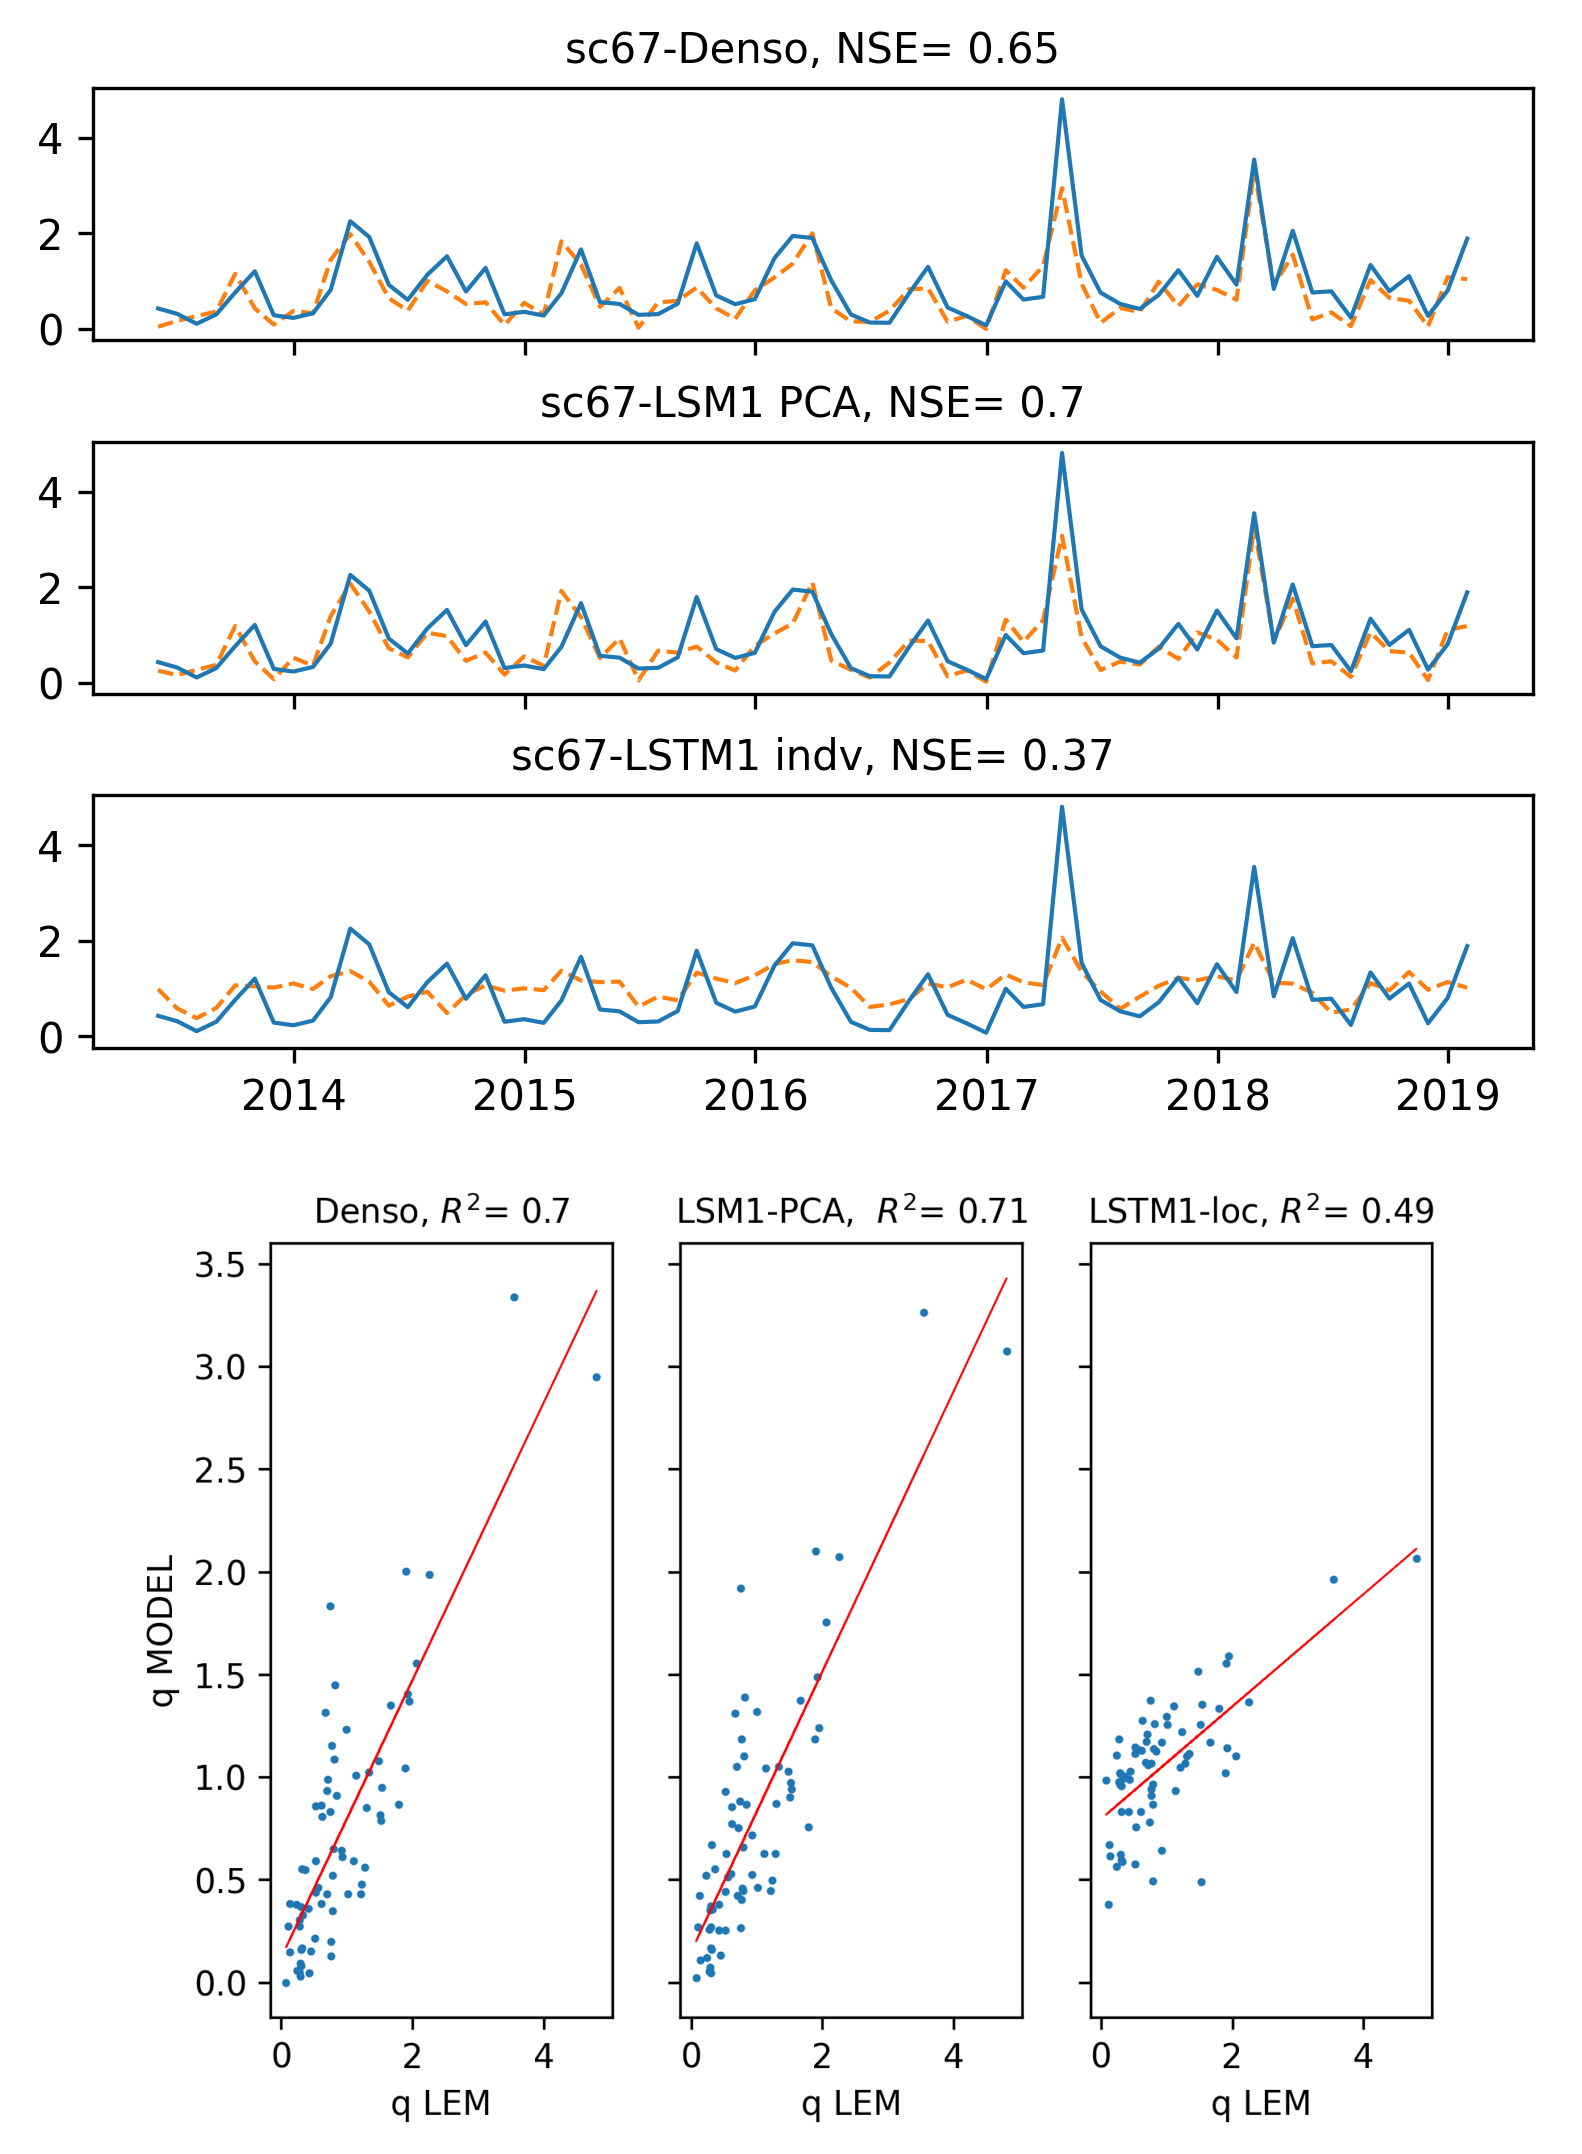
\includegraphics[height=6.in]{Figures/comp_grilla/resultados_sc67.png}
    \caption{ Predicciones del caudal de descarga obtenidos con los modelos Denso, 
    LSTM1 con PCAs y LSTM1 local en la subcuenca con id 67. En los
    paneles inferiores se muestran los grados de ajuste correspondientes.}
    \label{alcomp67}
  \end{center}
\end{figure}

En la figura \ref{alcomp67} se muestra  a modo de ejemplo un caso en el que el modelo LSTM1 loc falla 
al predecir los valores en el conjunto de test, mientras que los modelos Denso y LSTM1 PCA arrojan un ajuste aceptable
 ($NSE>0.6$). En este caso, el modelo LSTM1 loc ha sido capaz de reflejar 
cierta tendencia de los datos pero aún así la calidad del ajuste es baja ($NSE<0.5$). El modelo LSTM1 PCA, que 
posee ambas ventajas, la de considerar componentes principales y redes recurrentes, es capaz de predecir los valores de los caudales
en el conjunto de test con una calidad buena ($NSE=0.7$). 

 
\begin{figure}[h!]
\begin{center}
  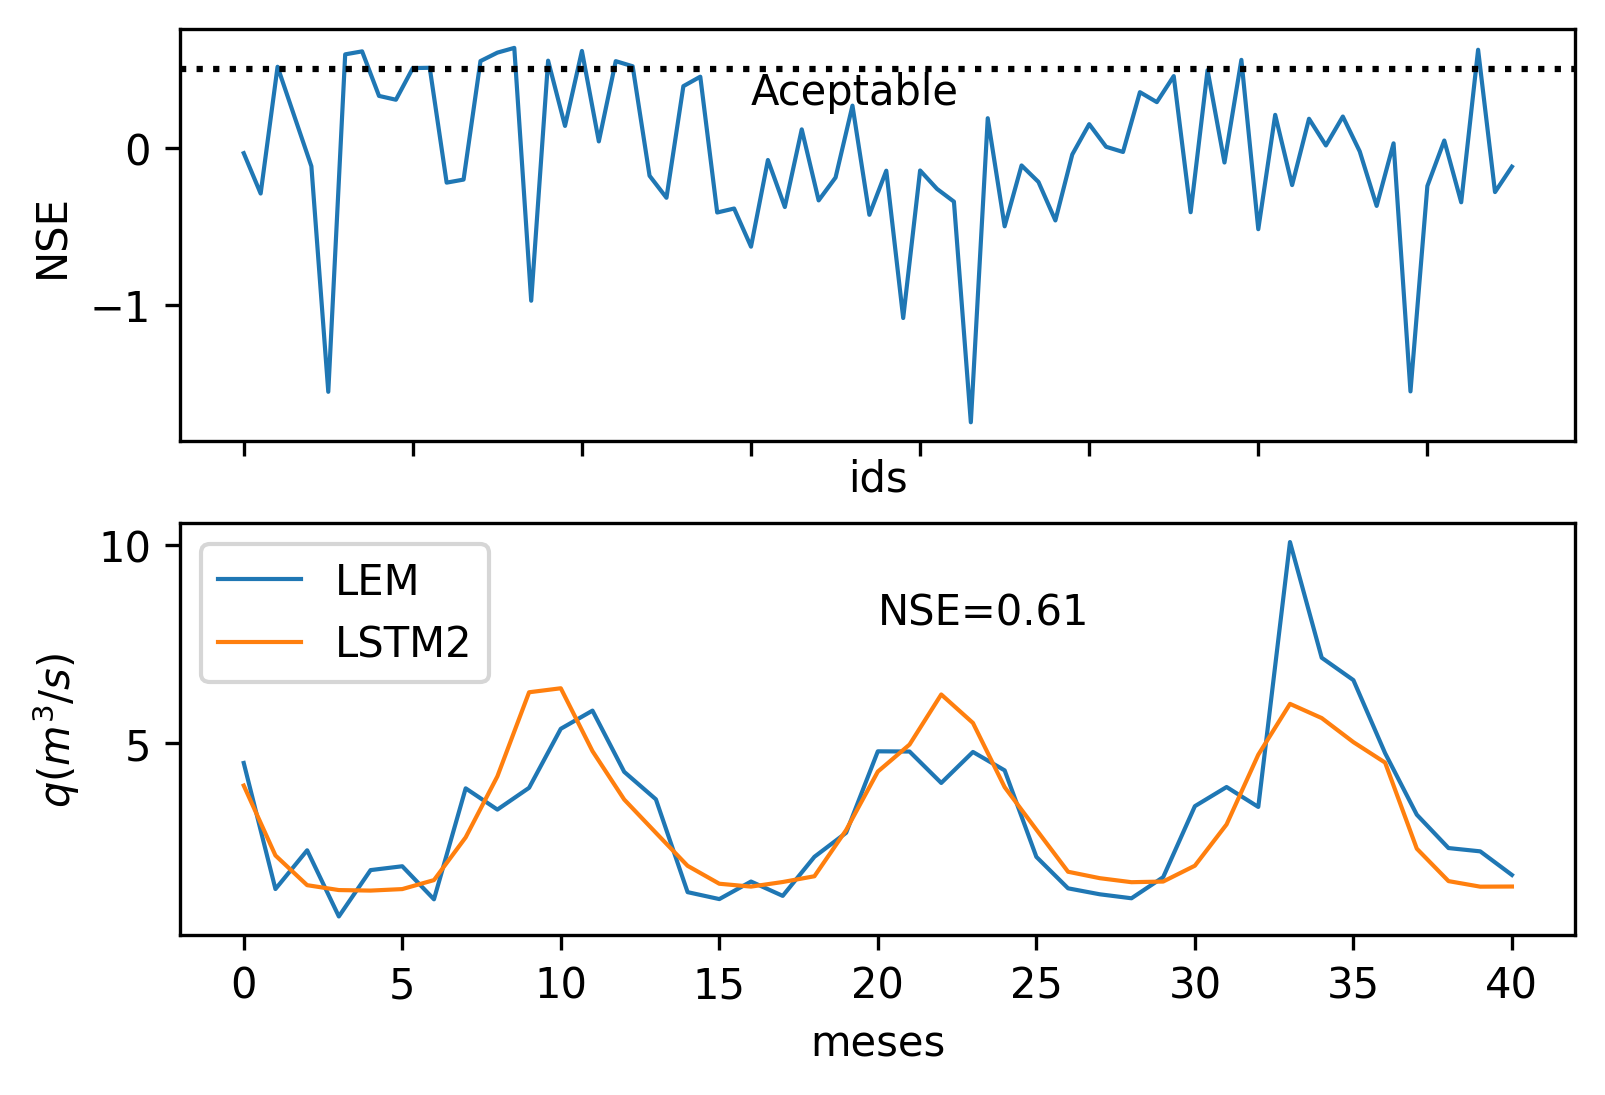
\includegraphics[height=2.8in]{Figures/seq/results_seq.png}

  \caption{ Resultados del Modelo LSTM2. En el panel superior se muestran los valores de NSE a lo largo de toda la cuenca y En
  el panel inferior, los valores predichos en la sub-cuenca con id 15. }
  \label{seq15}
\end{center}
\end{figure}

En la figura \ref{seq15} se muestran los resultados obtenidos para el modelo LSTM2 entrenado secuencialmente. 
en el panel superior se muestran lo valores del coeficiente NSE a lo largo de toda la cuenca
y en el panel inferior los resultados obtenidos para el mejor ajuste. Se puede observar que
la performance del modelo es en general bastante pobre, sólo unos pocos puntos sobrepasan en umbral de calidad aceptable.
Los mayores problemas que presenta esta aproximación es que por un lado los errores cometidos en cada una de las
predicciones es propagado y acumulado a lo largo del tiempo y por otro lado se pierde completamente
la información otorgada por las series hidro-climáticas de entrada, por lo cual el modelo no es capaz de aprender ningún 
patrón relacionado con la respuesta que las diferentes sub-cuencas tienen frente a las series de precipitación.  






%   \begin{center}
%     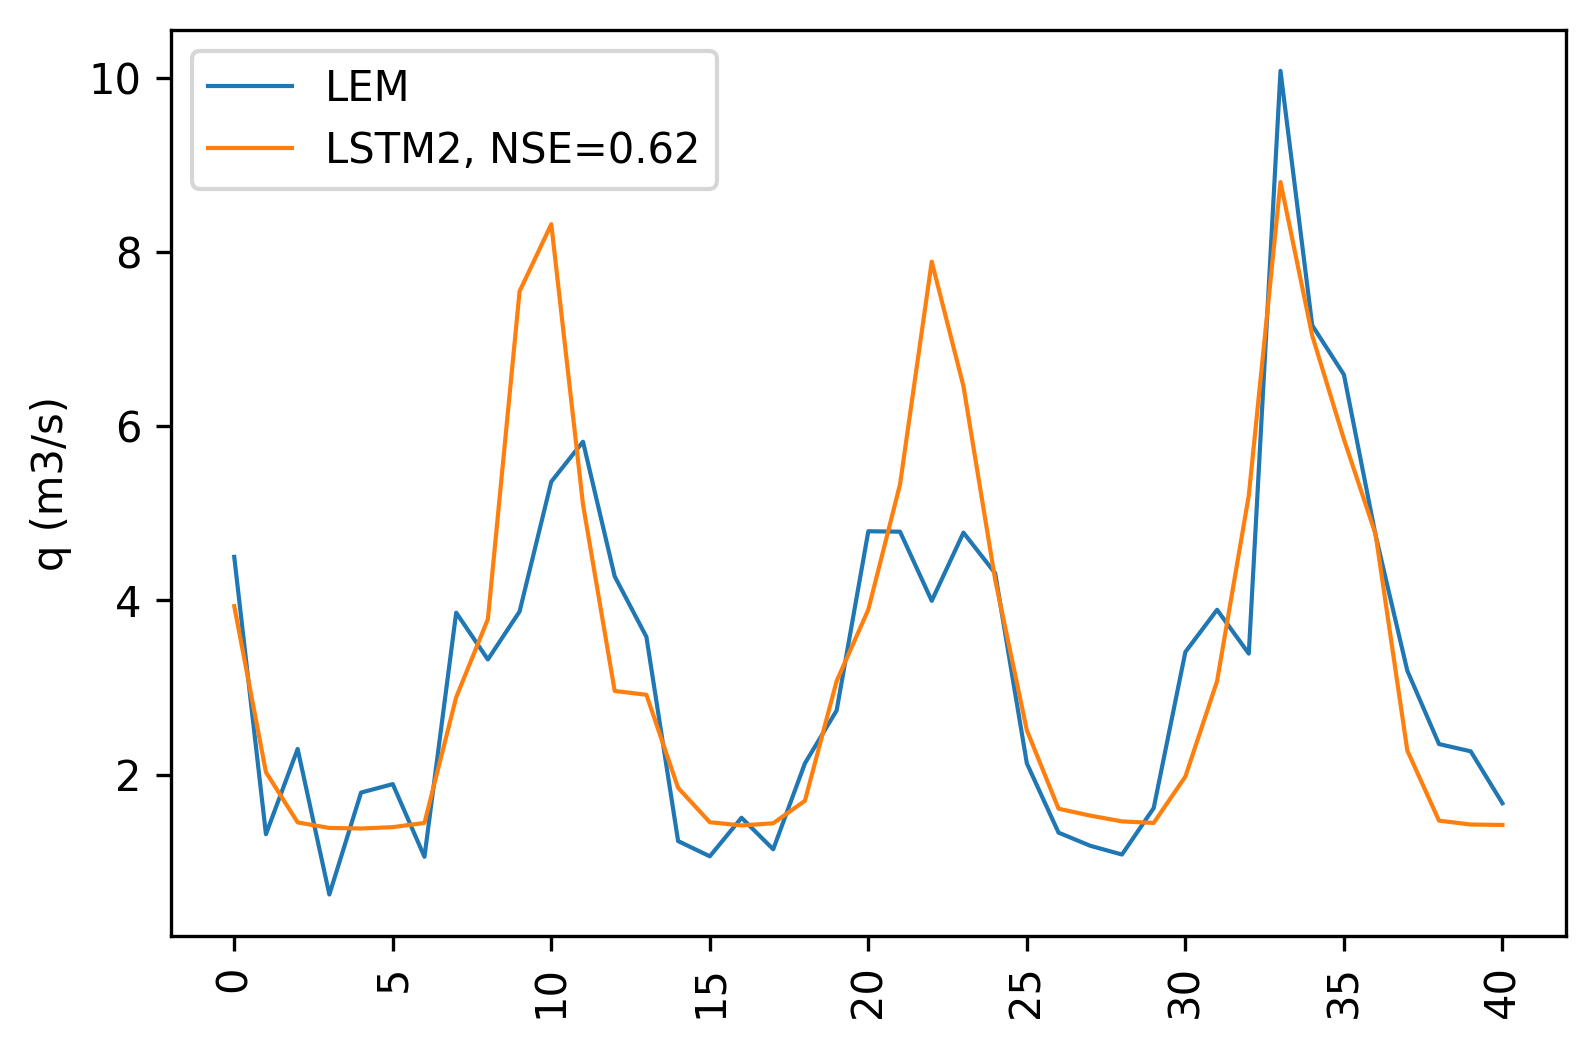
\includegraphics[height=2.5in]{Figures/seq/seq_sc15.png}
%     \caption{ Resultados del Modelo LSTM 2.}
%     \label{seq15}
%   \end{center}
% \end{figure}


% #* Graficas de las distribuciones de los pesos? para ver que patrones se forman?

% \begin{figure}[h!]
%     \begin{center}
%       \includegraphics[height=4.in]{Figures/comparacion_scs.png}
%       \caption{ Resultados del Modelo LSTM 2.}
%       \label{autocorrelacion}
%     \end{center}
%   \end{figure}





% \begin{figure}[h!]
%     \begin{center}
%       \includegraphics[height=3.5in]{Figures/autocorr_scs.png}
%       \caption{ Funciones de autocorrelación.}
%       \label{resultados_q}
%     \end{center}
%   \end{figure}

% En la figura \ref{autocorrelacion} se muestran las funciones de autocorrelación
% correspondientes a cada una de la subcuencas. Se puede observar que ambos modelos son capaces de captar correctamente 
% la estacionalidad de los datos.



%  \begin{figure}[h!]
%     \begin{center}
%       \includegraphics[height=3.in]{Figures/modelo_LSTM_seq.png}
%       \caption{ Resultados del modelo LSTM 3.}
%       \label{result_LSTM3}
%     \end{center}
%   \end{figure}


%   En la figura \ref{result_LSTM3} se muestran los resultados obtenidos con el modelo LSTM3 en todo el rango de datos 
%   para la subcuenca numero 73. En este enfoque, se han predicho los datos de manera secuencial, 
%   para lo cual sólo se ha utilizado la información de las series temporales de los caudales simulados en el
%   conjunto de entrenamiento. Si bien este modelo predice   correctamente la tendencia de los datos, 
%   falla al predecir los valores de los caudales.

  





% %   \begin{figure}[h!]
% %     \begin{center}
% %       \includegraphics[height=2.in]{Figures/NSEs_Delta prec.png}
% %       \caption{ Modelo LSTM 2}
% %       \label{Red_LSTM2}
% %     \end{center}
% %   \end{figure}

\section{Cálculo de balance hídrico con MODSIM}


Con el fin de determinar si los resultados obtenidos con redes neuronales pueden ser utilizados para simular 
operaciones en la cuenca CHRC, se ha determinado el balance hidrológico utilizando el software MODSIM (introducido en \ref{Modelo_balance})
con los caudales simulados por el modelo hidrológico MELCA y las predicciones de los modelos
de redes neuronales en el conjunto de test.

En el panel superior de la figura \ref{modsim}  se muestra el residuo ($R$), es decir la diferencia entre los valores de los 
caudales predichos respecto a los caudales de referencia (en este caso simulados con el modelo MELCA), 
para diferentes sub-cuencas distribuidas a lo largo de toda la cuenca hidrográfica Chambo. 
En los paneles inferiores se muestran los valores de los caudales  arrojados por MODSIM  para la sub-cuenca que se encuentra
a la salida de CHRC (aguas abajo) y para una de las sub-cuencas que se encuentra a mayor altitud (aguas arriba). 
Las curvas continuas corresponden al resultado obtenido con los caudales simulados con el modelo MELCA, 
y la curva a rayas es el resultado obtenido cuando consideramos los valores predichos por el modelo LSTM1 PCA. 
Se puede apreciar que los resultados arrojados por MODSIM son los mismos para ambos casos, es decir, 
las pequeñas variaciones mostradas en el panel superior no influyen en el resultado final. 



  \begin{figure}[h!]
    \begin{center}
      \includegraphics[height=6.5in]{Figures/modzim/comp_modzim.png}
      \caption{ Paneles superiores: residuos obtenidos a lo largo de diferentes sub-cuencas. 
      Paneles inferiores: resultados finales obtenidos utilizando el software de gestión de recursos MODSIM, teniendo en cuenta los usos del agua.}
      \label{modsim}
    \end{center}
  \end{figure}


  % \begin{figure}
%     \centering
%     \begin{subfigure}[b]{0.6\textwidth}
%         \centering
%         \includegraphics[width=\textwidth]{Figures/comparacion_denso_LSTM_NSE.png}
%         \caption{}
%         \label{fig:y equals x}
%     \end{subfigure}
%     \hfill
%     \begin{subfigure}[b]{0.6\textwidth}
%         \centering
%         \includegraphics[width=\textwidth]{Figures/comparacion_denso_LSTM_PBIAS.png}
%         \caption{}
%         \label{fig:three sin x}
%     \end{subfigure}
%        \caption{Three simple graphs}
%        \label{fig:three graphs}
% \end{figure}

%\chapter{Análisis de Escenarios}
\label{capitulo 3}
\chapter{Discusiones y Conclusiones}
\label{Discusiones y conclusiones}

Los resultados descritos en el capítulo anterior demuestran que el modelo que realiza los mejores ajustes es el LSTM1 cuando es entrenado en 
el espacio de las componentes principales. Aproximadamente un 70$\%$ de los ajustes obtenidos con el mismo son excelentes mientras que esta cifra  
desciende al 60$\%$ para los modelos denso y LSTM1 entrenado localmente. Si bien los últimos modelos poseen una buena performance en la mayoría de 
las sub-cuencas, presentan mucha variación en el coeficiente de NSE, alcanzando incluso valores negativos en algunos puntos para los cuales 
el modelo LSTM1 PCA arroja resultados que son desde aceptables hasta excelentes. Por otro lado el experimento realizado con el modelo LSTM2, que considera 
un entrenamiento secuencial utilizando solamente los valores de la serie de caudales de descarga de las sub-cuencas, ha demostrado
tener una  mala performance en la mayoría de los puntos. 

Los resultados antes mencionados nos llevan a concluir que la inclusión de las celdas de memoria LSTM y la presencia de componentes principales 
mejoran notablemente la performance de los modelos en cuencas hidrográficas. 
Por un lado las celdas LSTM permiten almacenar información de eje temporal sobre los diferentes procesos  que ocurren en  las sub-cuencas,
y así captar más información sobre la relación entre eventos de precipitación y descarga. Por otro lado, 
las componentes principales reducen considerablemente la dimensión del espacio predictor
y combinan la información proveniente de todo el dominio del mismo, lo que soluciona problemas de sobre ajustes y el problema
des desvanecimiento del loss presente en las cuencas más pequeñas y áridas. 
Finalmente, una vez entrenados lo modelos, se ha demostrado que los resultados obtenidos con redes LSTM
pueden ser utilizados para simular operaciones en la cuenca CHRC, ya que se ha comprobado que
el resultado del balance hidrológico obtenido con MODSIM es el mismo que los obtenidos con los valores simulados por el modelo LEM.

Todos estos resultados apuntan en la misma línea que estudios recientes en los cuales se concluye que 
las redes neuronales generalmente requieren una gran cantidad de datos de entrenamiento y que 
los ajustes que se obtienen al entrenar modelos de aprendizaje profundo en una sola sub-cuenca no suelen ser fiables \cite{Kratzert}. 
Esto supone una gran diferencia con el modelado y calibrado hidrológico tradicional que normalmente demuestra una mejor performance 
cuando los modelos se calibran de forma independiente para cada sub-cuenca.
Ésta propiedad de los modelos clásicos presenta problemas, ya que se ha observado que los 
 parámetros obtenidos por extrapolaciones  basadas en valores calibrados en cuencas de referencia 
pueden dar lugar a espacios de parámetros poco realistas\cite{Mizukami}. 
Los modelos LSTM en cambio, demuestran tener la capacidad de aprender simultáneamente relaciones de series temporales 
y espaciales en el mismo marco predictivo, lo que evita muchos problemas que actualmente se encuentran 
asociados con la estimación y transferencia de parámetros de modelos hidrológicos tradicionales \cite{Kratzert}, \cite{nearing}.

Una conclusión importante es entonces que las celdas LSTM son capaces de generar un modelo único a partir de grandes conjuntos de datos  
capaz de reflejar los comportamientos hidrológicos regionales específicos de cada sub-cuenca
ya que estos modelos  vinculan las características locales de las sub-cuencas y aprenden
un modelo general a partir de los datos combinados de todas ellas. 
Es por esto que concluimos que la principal virtud de las redes neuronales no es simplemente el hecho de que ajusten bien sino su capacidad de
aprendizaje y  flexibilidad para ser utilizadas en una variedad de  lugares y condiciones diferentes.


Por último, como posibles mejoras para trabajos futuros se propone concatenar los descriptores estáticos de las sub-cuencas, 
como por ejemplo el área, la longitud del cauce, etc., al espacio predictor. Otra mejora podría ser definir una función objetivo al 
entrenar los modelos que no dependa del valor medio de los caudales de descarga de las diferentes cuencas. Kratzert etal. \cite{Kratzert} 
proponen por ejemplo usar directamente una definición global del coeficiente de Nash-Stutcliffe durante el entrenamiento
de los datos. En este caso, si bien se perdería la linelidad entre las métricas del RMSE y el NSE,  esto permitiría 
contemplar el hecho de que las variancias de los datos observacionales difieren en distintas cuencas y así evitar el sobre-peso 
asociado a las cuencas más grandes y húmedas.

\chapter{Anexo}
\label{Desarrollo}
Con el fin de poder ejecutar los modelos ANNs desarrollados y calcular el balance hídrico de la cuenca, 
se han creado dos aplicaciones REST APIs utilizando la librería flask de python \cite{flask}. La idea 
es que mediante la correcta estructuración de los datos de entrada necesarios para la ejecución de los modelos, estos se puedan ejecutar en diferentes 
cuencas.
Para esto se han creado diferentes clases y métodos en python que constituyen el core de la API, estos métodos o recursos se hacen 
accesibles a través de la interfaz de la API, en la que se exponen los métodos y las URLs disponibles para acceder 
y/o manipular cada uno de ellos.


El proceso que se ha seguido para crear esta API es el siguientes:


\begin{itemize}
    \item En primer lugar se ha construido una base de datos relacional que contiene los descriptores las cuencas hidrográficas (Fig. \ref{BD}), así como 
   también todos los datos referentes a los diferentes usos de agua. Esta base de datos fue realizada con el software PostgreSQL  un sistema 
   de código abierto de administración de bases de datos del tipo relacional cuyas consultas  se basan en SQL\cite{PostgretSQL}.
   Por otro lado las series temporales que actúan como inputs de los modelos no admiten consultas relacionales y por lo tanto 
   se han almacenado de forma separada en archivos de excel en un directorio local. 
   \item Una vez estructurados los datos en sus diferentes formatos, se ha desarrollado una serie de métodos en python para hacer todo tipo de consultas,
   agregaciones, actualizaciones, y borrado de los datos. Para esto se utilizó la librería psycopg2, una de las librerías más populares que sirven para 
   integrar el lenguaje de PostgreSQL en python y permite crear métodos que hagan consultas en la base de datos creada con dicho software.
   \item El tercer paso es crear una API que contenga todos los métodos que faciliten el acceso a los datos, entre los métodos creados se destacan 
   métodos que 
   permiten recorrer la navegación de la cuenca, encontrar para una cuenca dada,  las cuencas aguas arriba que vierten en ella,
    todas las demandas y aportaciones de agua, etc (Fig. \ref{BD}).
    \item Una vez creara la API que contiene los métodos que permiten la consulta de la base de datos y las series temporales, 
    se ha creado otra aplicación que ejecuta los modelos desarrollados (Fig. \ref{MELCA}). Para esto se ha creado una clase python, que posee varios métodos, 
    que ejecutan los modelos, y calculan el balance hídrico de la cuenca. Para esto es necesario utilizar la librería
    la librería request que permite hacer peticiones HTTP POST y GET a la base de datos que contiene las tablas con las series temporales y 
    los descriptores necesarios para la ejecución de los modelos.
    \item Por último, una vez que se ha accedido a todos los datos necesarios para ejecutar los modelos que simulan/predicen los caudales
    naturales de las cuencas, y los datos asociados a todas las demandas y aportaciones de agua, 
    se procede a  calcular el balance hídrico de la cuenca siguiendo los pasos:
    \begin{enumerate}
        \item para una subcuenca dada, se agregan los resultados de las simulaciones de caudal aguas arriba siguiendo el cauce de 
        navegación de la cuenca,
        \item se averiguan todas las demandas que toman agua de dicha cuenca y todas las demandas que retornan agua a la misma,
        \item se calcula el balance como: $q_{ac}-q_{dem}+q_{ret}$, donde $q_{ac}$ el caudal natural agregado aguas arriba, $q_{dem}$ el caudal 
        agregado de todas las demandas y $q_{ret}$ el retorno total de todas las demandas.
    \end{enumerate}  
\end{itemize}


\begin{figure}[h!]
    \begin{center}
      \includegraphics[height=7.in]{Figures/BD_diagram.png}
      \caption{ Base de datos relacional con los descriptores de las componentes de una cuenca hidrográfica. }
      \label{BD}
    \end{center}
  \end{figure}

  \begin{figure}[h!]
    \begin{center}
      \includegraphics[height=4.in]{Figures/potable water demands.PNG}
      \caption{ Ejemplo de consulta de uno de los métodos de la API que contiene la base de datos. }
      \label{BD}
    \end{center}
  \end{figure}

  

  \begin{figure}[h!]
    \begin{center}
      \includegraphics[height=7.in]{Figures/consulta_MELCA.png}
      \caption{ Ejemplo de consulta del método que calcula el balance hídrico de la cuenca. }
      \label{MELCA}
    \end{center}
  \end{figure}


% por un lado se ha construido una base de datos relación



% , así como los parámetros necesesarios para ejecutar los modelos 

% Para esto se han desarrollado dos aplicaciones con la librería flask de python. Una aplicación que contienen una serie de métodos que permiten 
% hacer una consulta de los descriptores de las cuencas hidrográficas y las series temporales necesarias para ejecutar los modelos. 

% Para esto se ha creado una base de datos relacional (Fig. ---) que contiene los descriptores de las cuencas, así como tambien
% todos los datos referentes a los diferentes usos de agua utilizando el software postgresql,  un sistema de código abierto de 
% administración de bases de datos del tipo relacional, aunque también es posible ejecutar consultas que sean no relaciones. 
% En este sistema, las consultas relacionales se basan en SQL, mientras que las no relacionales hacen uso de JSON.

% y la librería psycopg2,
% una de las librerías más populares que sirven para integrar el lengaje de PostgreSQL en python y permite crear métodos que hagan consultas en la base
% de datos creada con dicho software.

% Los métodos creados permiten consultar, agregar, eliminar y actualizar los diferentes componentes de CHRC, 
% así como obtener información de la estructura de la cuenca permitiendo reconstruir el recorrido del agua entre los diferentes cauces.

% En la figura ---se muestran a modo de ejemplo algunos de los métodos de la API creada. 
% El objetivo de crear esta api es el de facilitar la ejecución de los modelos en otras cuencas hidrográficas.

% Una vez creara la API que contiene la base de datos, se ha creado otra aplicacion, tambien con python y con la 
% libreria flaskj que contiene dos metodos, uno para ejecutar el modelo MELCA y otro para ejecutar el modelo LSTM1 PCA. 
% Para esto se ha utilizado la libreria request para hacer consultas a la api que contiene la base de datos y los inputs de los modelos.

% En esta aplicacion se ha utilzado la libreria de pandas para convertir los resultados de las consultas de la BD a datasets
% de panda y facilitar operaciones como la agregacion de las cuencas aguas arriba siguiendo la estructura de la red, 
% agilizar las consultas de las demandas de agua y poder calcular el equilibrio hidrico de todo el sistema.



 \bibliographystyle{babunsrt}
 \bibliography{bibliografia}

\end{document}